%
% main.tex
%
% Copyright The GOLDS-UFSC Contributors.
%
% GOLDS-UFSC Documentation
%
% This work is licensed under the Creative Commons Attribution-ShareAlike 4.0
% International License. To view a copy of this license,
% visit http://creativecommons.org/licenses/by-sa/4.0/.
%

%
% \brief Main file.
%
% \author Gabriel Mariano Marcelino <gabriel.mm8@gmail.com>
%
% \version 0.3.0
%
% \date 2020/06/05
%

\documentclass[a4paper,12pt]{book}

\usepackage{spacelab_book}

\title{Radio Occultation Design and Mission Overview}
\author{SpaceLab}
\date{\today}

% File metadata
\hypersetup
{
    pdfauthor   = {SpaceLab},
    pdfsubject  = {\thetitle},
    pdftitle    = {\thetitle},
    pdfkeywords = {Nanosatellites, CubeSats, GOLDS-UFSC}
}

\begin{document}

    \pagenumbering{roman}
    \setcounter{page}{1}

    %
% titlepage.tex
%
% Copyright The GOLDS-UFSC Contributors.
%
% GOLDS-UFSC Documentation
%
% This work is licensed under the Creative Commons Attribution-ShareAlike 4.0
% International License. To view a copy of this license,
% visit http://creativecommons.org/licenses/by-sa/4.0/.
%

%
% \brief Title page.
%
% \author Gabriel Mariano Marcelino <gabriel.mm8@gmail.com>
%
% \version 0.3.0
%
% \date 2020/06/05
%

\begin{titlepage}

\thispagestyle{empty}

\begin{flushleft}
SpaceLab.DMO.2025.04.29 rev 0.0
\end{flushleft}

\vspace{1cm}

\begin{figure}[!ht]
    \begin{flushleft}
        
\includegraphics[width=7cm]{figures/spacelab-logo-full-color-rgb-1000px@72ppi.png}
    \end{flushleft}
\end{figure}

\begin{flushleft}
\Huge{\textbf{\thetitle}}
\rule[0pt]{\textwidth}{5pt}
\end{flushleft}

\vspace{0.2cm}

\begin{flushleft}
%\textit{\thetitle} \\
\textit{SpaceLab, Universidade Federal de Santa Catarina, Florianópolis - Brazil}
\end{flushleft}

\vfill
\vfill

\begin{flushright}
April 2025
\end{flushright}

\end{titlepage}

    \cleardoublepage
    %
% authorpage.tex
%
% Copyright The GOLDS-UFSC Contributors.
%
% GOLDS-UFSC Documentation
%
% This work is licensed under the Creative Commons Attribution-ShareAlike 4.0
% International License. To view a copy of this license,
% visit http://creativecommons.org/licenses/by-sa/4.0/.
%

%
% \brief Author page.
%
% \author Gabriel Mariano Marcelino <gabriel.mm8@gmail.com>
%
% \version 0.3.0
%
% \date 2020/06/05
%

\thispagestyle{empty}

\begin{center}

\textbf{\thetitle}

\textit{April, 2025}

\vspace{1cm}

\textbf{Project Chief:}

Eduardo Augusto Bezerra

\vspace{1cm}

\textbf{Authors:}

Yunior Alcantara Guevara \\
Authors... \\

\vspace{1cm}

\textbf{Contributing Authors:}

Eduardo Augusto Bezerra \\

\vspace{1cm}


\textbf{Revision Control:}

\end{center}

\begin{table}[!ht]
    \begin{center}
        \begin{tabular}{cL{5cm}L{5.5cm}C{2cm}}
            \toprule[1.5pt]
            \textbf{Version} & \textbf{Author}  & \textbf{Changes}    & \textbf{Date} \\
            \midrule
            0.0     & Y. A. G & Document creation   & 2025/04/29 \\
            0.x     & ... & First release       & 202x/xx/xx \\
            0.x     &  ... & CDR release      & 202x/xx/xx \\
        \end{tabular}
    \end{center}
\end{table}

\vfill

\begin{figure}[!h]
	\begin{center}
		\includegraphics[width=0.25\textwidth]{figures/by-sa.eps}
	\end{center}
\end{figure}

\textcopyright\  2025 by SpaceLab. \thetitle. This work is licensed under the Creative Commons Attribution-ShareAlike 4.0 International License. To view a copy of this license, visit \href{http://creativecommons.org/licenses/by-sa/4.0/}{http://creativecommons.org/licenses/by-sa/4.0/}.

    \cleardoublepage

    \listoffigures
    \addcontentsline{toc}{chapter}{List of Figures}

    \listoftables
    \addcontentsline{toc}{chapter}{List of Tables}

    \printnomenclature
    \addcontentsline{toc}{chapter}{Nomenclature}

    \tableofcontents
    \cleardoublepage
    
    \pagenumbering{arabic}
    \setcounter{page}{1}

    %
% introduction.tex
%
% Copyright The Radio Occultation Contributors.
%
% Radio Occultation Documentation
%
% This work is licensed under the Creative Commons Attribution-ShareAlike 4.0
% International License. To view a copy of this license,
% visit http://creativecommons.org/licenses/by-sa/4.0/.
%

%
% \brief Introduction chapter.
%
% \author Gabriel Mariano Marcelino <gabriel.mm8@gmail.com>
%
% \institution Universidade Federal de Santa Catarina (UFSC)
%
% \version 0.2.0
%
% \date 2020/06/05
%

\chapter{Introduction} \label{ch:introduction}

Radio Occultation is a 2U CubeSat (10$\times$10$\times$22.70 cm), and it is a follow up of Radio Occultation mission \cite{floripasat}. Both Radio Occultation and Radio Occultation are developed by SpaceLab/UFSC \cite{spacelab}. Radio Occultation main payload is the EDC board (\textit{Environmental Data Collection}) \cite{edc}, developed by INPE\nomenclature{\textbf{INPE}}{\textit{Instituto Nacional de Pesquisas Espaciais.}}. The mission is part of the ``GOLDS\nomenclature{\textbf{GOLDS}}{\textit{Global Open Collecting Data System.}}'' constellation (``Global Open Collecting Data System''), a collaborative CubeSat constellation for environmental data collection planned as part of the Brazilian Space Program \cite{golds}.

The project started just after the launch of Radio Occultation (first half of 2020) and is planned to be launched in 2023. Most of the embedded electronics is partially or totally based on the Radio Occultation satellite, with the same and/or improved versions of the modules. In other words, this project has, at some level, a flight heritage.

A conceptual image of the Radio Occultation satellite is shown in \autoref{fig:Radio Occultation-render}.

\begin{figure}[!ht]
    \begin{center}
        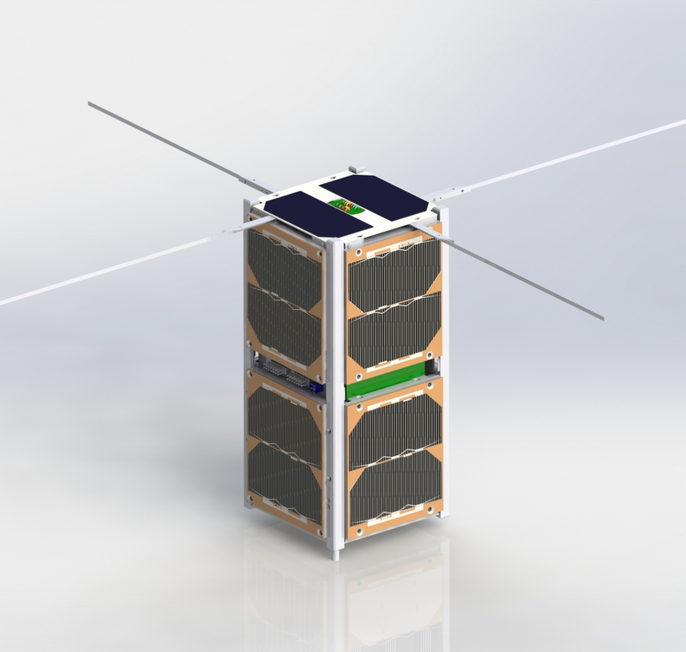
\includegraphics[width=0.7\textwidth]{figures/floripasat-2.jpg}
        \caption{Radio Occultation 3D renderization.}
        \label{fig:Radio Occultation-render}
    \end{center}
\end{figure}

\section{Mission Description}
The mission's main objective is the In-Orbit Validation (IoV) of INPE's EDC payload, using a service module based on Radio Occultation bus. The EDC payload is a module developed for CubeSats and capable of receiving data from data collection stations (Plataformas de Coleta de Dados, PCDs) of the Brazilian Data Collection System (\textit{Sistema Brasileiro de Coleta de Dados}, SBCD) installed along the Brazilian territory. The received data is forwarded to the ground segment through the main communication link offered by the satellite service module. A scientific contribution of the mission is the evaluation of radiation effects on electronic devices, as both EDC and the service platform are based on COTS. The radiation effects evaluation will be performed by the Radiation instrument, which has also been developed for the Radio Occultation mission. The mission provides also a relay service to the amateur radio community.
% The mission consists of testing the EDC payload developed by INPE in a real space mission, using for this, part of the flight heritage obtained during the Radio Occultation mission.

% The EDC payload is a module developed for CubeSats and capable of capturing data from data collection stations (PCDs) of the Brazilian Data Collection System (SBCD, or \textit{Sistema Brasileiro de Coleta de Dados}) installed along the Brazilian territory. The collected data can be retrieved through the main communication link offered by the satellite service modules. This mission will first use the EDC module in a space environment.

% As a secondary mission, we also intend to test other payloads, such as Payload-X, which is composed of a radiation-tolerant FPGA and a Radiation instrument using SRAM memories. These payloads, being secondary, will only be used for limited periods and upon request by telecommand.

\section{Mission Objectives}

The main objectives of the mission are as follows:

\begin{enumerate}
    \item In-Orbit Validation (IoV) of INPE's EDC payload.
    \item Provide a flight model for the satellite's service platform, based on Radio Occultation bus.
    \item Set up the ground segment for the mission operation.
    \item Receive environmental data from ground (from EDC stations), and forward the collected data to the ground station.
    \item Validate core-satellite functions in orbit.
    \item Perform experiments on radiation effects in electronic components in orbit, evaluating the radiation levels affecting EDC and the service platform modules.
    \item Serve as a relay for amateur radio communications, contributing to the amateur radio community.
\end{enumerate}

\section{Project Members}

All people involved in the project are students, professors and researchers from Federal University of Santa Catarina (UFSC), the National Institute for Space Research (INPE) and the Brazilian Space Agency (AEB\nomenclature{\textbf{AEB}}{\textit{Agência Espacial Brasileira.}}).

A list with the current members directly related to the project (2022/10/24) can be seen in \autoref{tab:team-members}.

\begin{table}[!htb]
    \centering
    \begin{tabular}{lllc}
        \toprule[1.5pt]
        \textbf{Name} & \textbf{Title} & \textbf{Position} & \textbf{Institution} \\
        \midrule
        Anderson Wedderhoff Spengler        & Dr.       & Professor             & UFSC \\
%        Edemar Morsch Filho                 & Dr.       & Professor             & UNESP \\
        Eduardo Augusto Bezerra             & Ph.D.     & Professor             & UFSC \\
        Richard Demo Souza                  & Dr.       & Professor             & UFSC \\
        Xisto Lucas Travassos               & Dr.       & Professor             & UFSC \\
        Laio Oriel Seman                    & Dr.       & Researcher            & UFSC \\
        Rodrigo Leonardi                    & Dr.       & Researcher            & AEB \\
        José Marcelo Duarte                 & Dr.       & Researcher            & INPE \\
        Manoel Jozeane Mafra de Carvalho    & M.Sc.     & Researcher            & INPE \\
        % Cezar Antônio Rigo                  & Dr.       & Researcher            & UFSC \\
        Gabriel Mariano Marcelino           & M.Sc.     & Doctoral Student      & UFSC \\
        Brenda Fernandes Ribeiro            & M.Sc.     & Doctoral Student      & UFSC \\
        André Martins Pio de Mattos         & B.Eng.    & Doctoral Student      & UFSC \\
        Edilberto Costa Neto                & B.Eng.    & Master Student      & UFSC \\
        Vinicius Pimenta Bernardo           & B.Eng.    & Master Student      & UFSC \\
        Augusto Cezar Boldori Vassoler      & B.Eng.    & Master Student      & UFSC \\
        % Amanda Medeiros                   & -         & Undergraduate Student & UFSC \\
        Bruno Benedetti                     & -         & Undergraduate Student & UFSC \\
        Caique Sales Miranda Gomes          & -         & Undergraduate Student & UFSC \\
        % Daniel Baron                      & -         & Undergraduate Student & UFSC \\
        João Cláudio Elsen Barcellos        & -         & Undergraduate Student & UFSC \\
        %Lorenzo Maturano                   & -         & Undergraduate Student & UFSC \\
        Lucas Zacchi                        & -         & Undergraduate Student & UFSC \\
        Matheus Wagner                      & -         & Undergraduate Student & UFSC \\
        %Maurício Sinigaglia                & -         & Undergraduate Student & UFSC \\
        Miguel Böing                        & -         & Undergraduate Student & UFSC \\
        Ramon de Araújo Borba               & -         & Undergraduate Student & UFSC \\
        % Tatiane dal Ross                  & -         & Undergraduate Student & UFSC \\
        Rebecca Quintino do O               & -         & Undergraduate Student & UFSC \\
        Vitória Beatriz Bianchin            & -         & Undergraduate Student & UFSC \\
        % Yan Castro de Azeredo             & -         & Undergraduate Student & UFSC \\
        \bottomrule[1.5pt]
    \end{tabular}
    \caption{Project members (2022/10/24).}
    \label{tab:team-members}
\end{table}

All the modules and methods used in this project are based in past works, mainly the Radio Occultation and the EDC projects. The list with the indirectly involved people is much bigger.

\section{Mission Patch}

The mission patch of the Radio Occultation can be seen in \autoref{fig:mission-patch}; it is inspired by the Radio Occultation patch \cite{floripasat} as it uses the flight heritage from its core modules (EPS, OBDH, TTC), which have been improved at hardware and/or software levels, to achieve the new requirements. The patch shows Brazil, the country of the mission's origin, gray orbits representing a constellation of CubeSats, and the yellow circles representing the "gold" color as a reference to the GOLDS constellation.

\begin{figure}[!htb]
    \begin{center}
        
\includegraphics[width=0.45\textwidth]{figures/golds-ufsc-patch.png}
        \caption{Radio Occultation mission patch.}
        \label{fig:mission-patch}
    \end{center}
\end{figure}

    %
% management.tex
%
% Copyright The Radio Occultation Contributors.
%
% Radio Occultation Documentation
%
% This work is licensed under the Creative Commons Attribution-ShareAlike 4.0
% International License. To view a copy of this license,
% visit http://creativecommons.org/licenses/by-sa/4.0/.
%

%
% \brief Mission management chapter.
%
% \author Gabriel Mariano Marcelino <gabriel.mm8@gmail.com>
%
% \version 0.2.0
%
% \date 2021/07/15
%

\chapter{Mission Management} \label{ch:management}

This chapter presents the main aspects of the general management of the project, like the mission schedule, product tree, and so on.


\section{Schedule}

The current schedule of the project is available in \autoref{tab:mission-schedule}.

\begin{table}[!h]
    \centering
    \begin{tabular}{cC{1.2cm}C{1.2cm}C{1.2cm}C{1.2cm}C{1.2cm}C{1.2cm}C{1.2cm}C{1.2cm}C{1.2cm}C{1.2cm}}
        \toprule[1.5pt]
        \multirow{4}{*}{\textbf{Activity}} & \multicolumn{8}{c}{\textbf{Month}} \\
                & Nov & Dez & Jan & Feb & Mar & Apr & May & Jun \\
                & 22  & 22  & 23  & 23  & 23  & 23  & 23  & 23  \\
        \midrule
        1       & \fc & \fc &     &     &     &     &     &     \\
        2       & \fc & \fc & \fc & \fc &     &     &     &     \\
        3       & \fc & \fc & \fc &     &     &     &     &     \\
        4       &     &     &     & \fc & \fc &     &     &     \\
        5       &     &     &     &     & \fc &     &     &     \\
        6       &     &     & \fc & \fc &     &     &     &     \\
        7       &     &     &     &     & \fc &     &     &     \\
        8       &     &     &     &     & \fc & \fc &     &     \\
        9       &     &     &     &     &     & \fc & \fc &     \\
        10      &     &     &     &     &     &     & \fc & \fc \\
        11      &     & \fc &     &     &     &     &     &     \\
        12      &     &     & \fc &     &     &     &     &     \\
        % 13      &     &     &     &     &     &     &     &     &     &     & \fc & \fc & \fc & \fc \\
        % 14      &     &     &     &     &     &     &     &     &     &     &     &     & \fc & \fc \\
        \bottomrule[1.5pt]
    \end{tabular}
    \caption{Mission schedule (updated on 2022/10/24).}
    \label{tab:mission-schedule}
\end{table}

Each activity of \autoref{tab:mission-schedule} is described below:

\begin{enumerate}
    \item Integration of the engineering model in SpaceLab UFSC.
    \item Preparation and suitability of the ground segment.
    \item Verification and validation of the engineering model.
    \item Integration and verification with data collection platforms.
    \item Verification and validation tests of Engineering Model compatibility with EMMN in the INPE / CRN in Natal.
    \item Verification and validation of the flight model.
    \item Environmental tests at the Integration and Testing Laboratory (LIT/INPE).
    \item Flight model acceptance and ground segment review.
    \item Ground segment delivery.
    \item Flight model delivery.
    \item Purchase (flight model).
    \item Delivery of purchased items (flight model).
\end{enumerate}

\section{Product Tree}

The product tree of the Radio Occultation mission is the project breakdown into successive levels of hardware and software products (or elements). The product tree of the project can be seen in the diagram of \autoref{fig:product-tree}. As shown, the satellite was divided into eight segments.

\begin{figure}[!ht]
    \begin{center}
        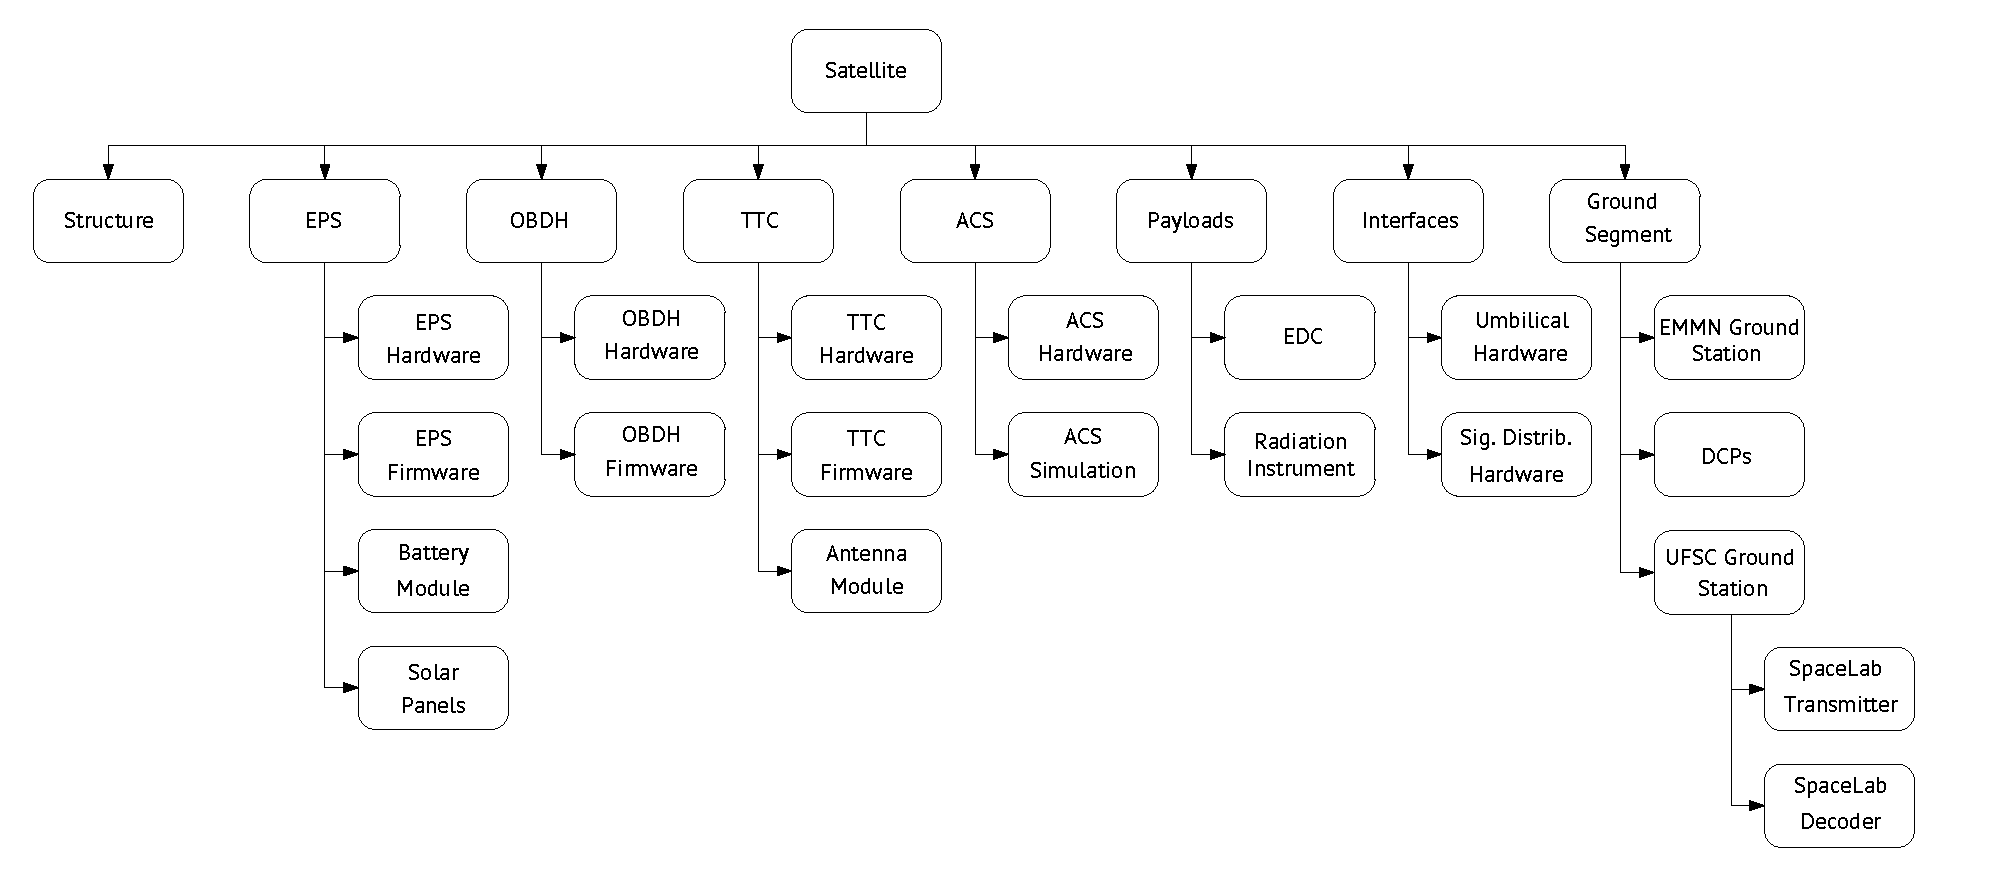
\includegraphics[width=\textwidth]{figures/product-tree.pdf}
        \caption{Product tree of the satellite.}
        \label{fig:product-tree}
    \end{center}
\end{figure}

The responsibility of each segment of the product tree is described next:

\begin{itemize}
    \item \textbf{Structure}: UFSC (COTS\nomenclature{\textbf{COTS}}{\textit{Commercial Off-The-Shelf}.}).
    \item \textbf{EPS}: UFSC (developed in-house, with COTS solar panels).
    \item \textbf{OBDH}: UFSC (developed in-house).
    \item \textbf{TTC}: UFSC (developed in-house).
    \item \textbf{ACS}: UFSC (developed in-house).
    \item \textbf{Payload EDC}: INPE
    \item \textbf{Radiation instrument}: UFSC (developed in-house).
    \item \textbf{Interfaces}: UFSC (developed in-house).
    \item \textbf{Ground segment}:
    \begin{itemize}
        \item \textbf{EMMN ground station}: INPE
        \item \textbf{DCPs}: INPE/SINDA and other institutions
        \item \textbf{UFSC ground station}: UFSC
    \end{itemize}
\end{itemize}

\subsection{Work Breakdown Structure}

The Work Breakdown Structure (WBS\nomenclature{\textbf{WBS}}{\textit{Work Breakdown Structure.}}) is presented as a diagram in \autoref{fig:wbs}. The WBS is divided into work packages (WP\nomenclature{\textbf{WP}}{\textit{Work Package.}}) as can be seen in the diagram. The description of each WP is detailed below.

\begin{figure}[!ht]
    \begin{center}
        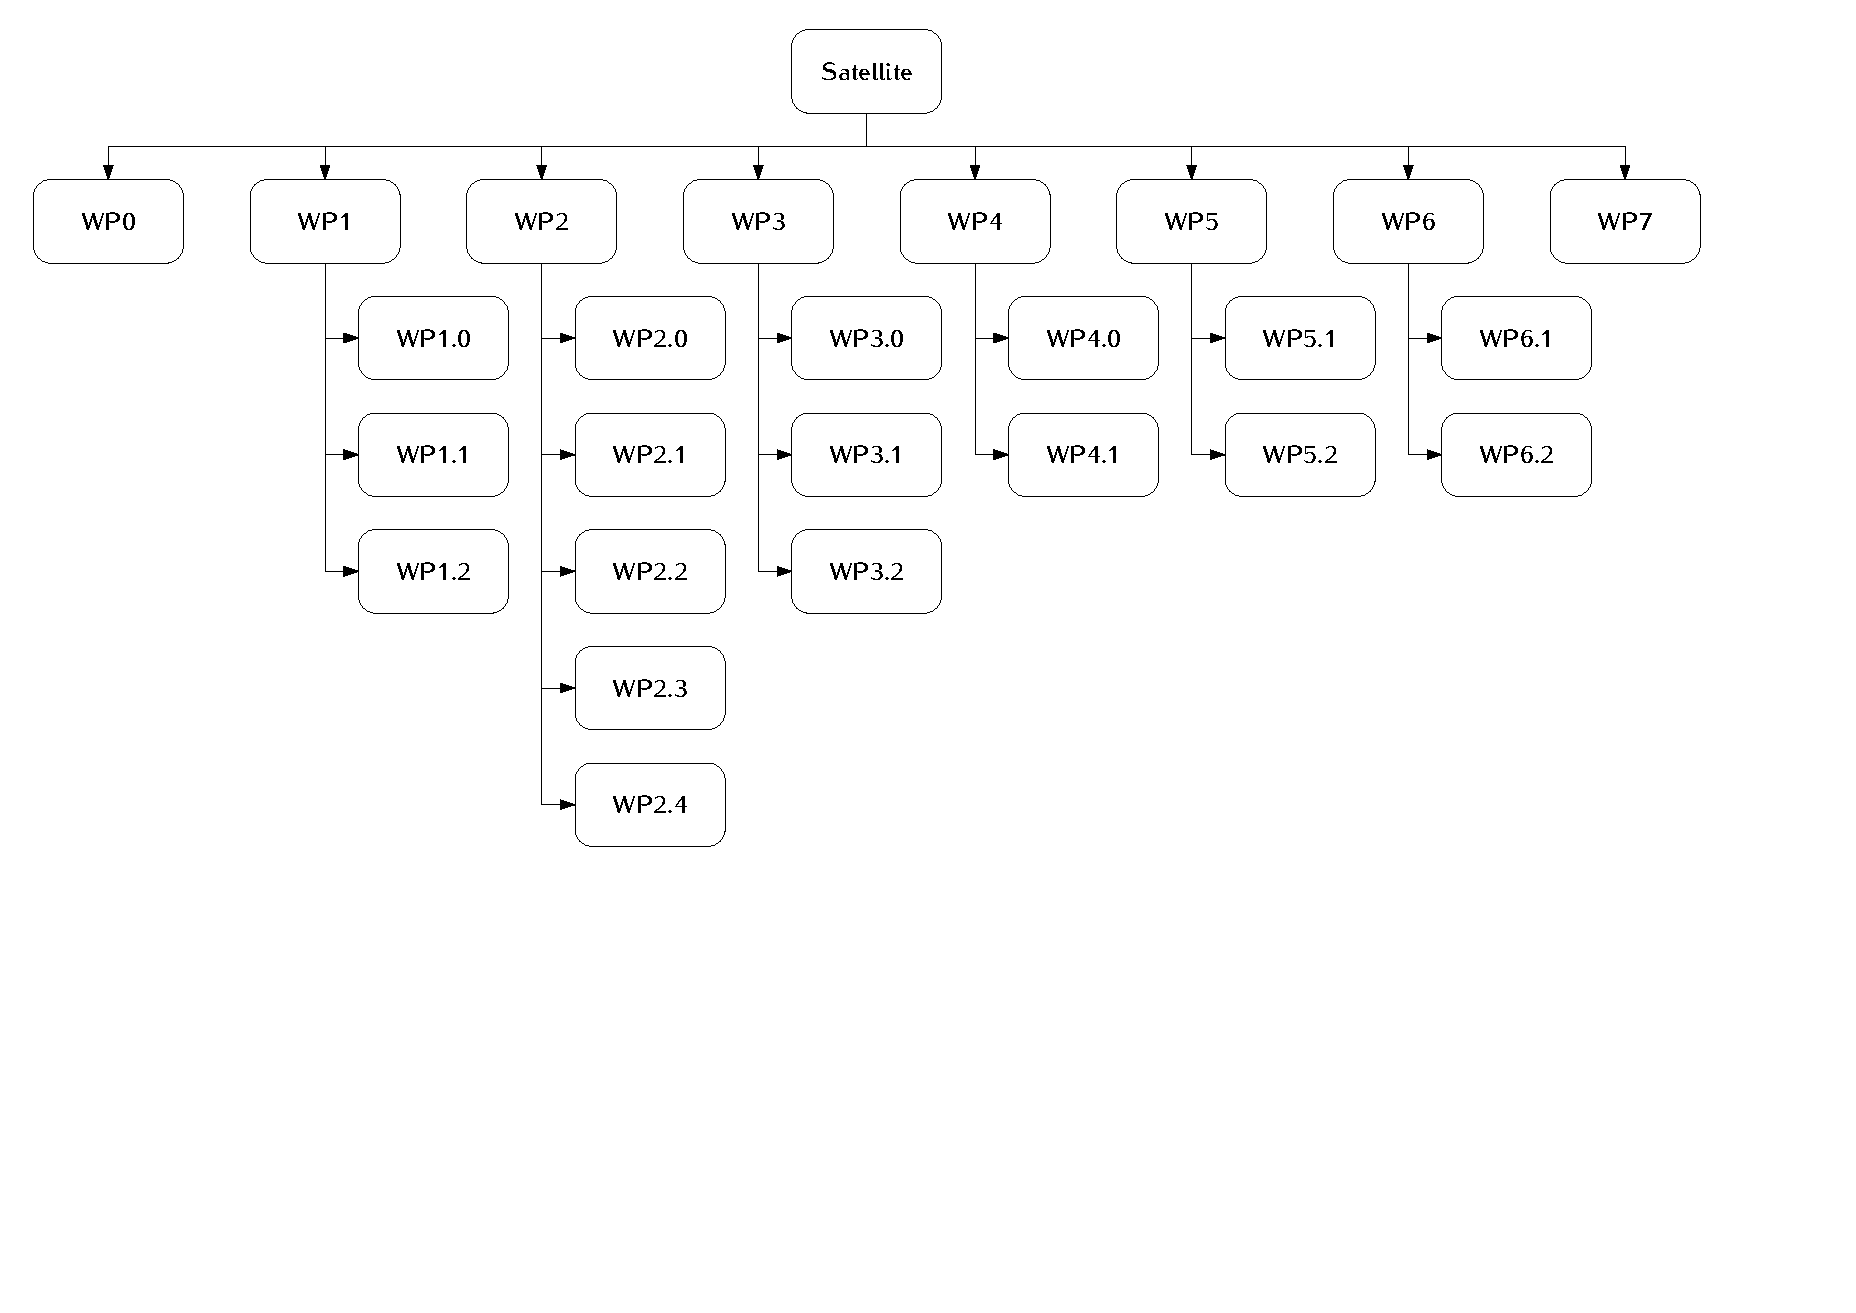
\includegraphics[width=\textwidth]{figures/wbs.pdf}
        \caption{WBS diagram.}
        \label{fig:wbs}
    \end{center}
\end{figure}

\begin{itemize}
    \item \textbf{WP0}: Management and preparation.
    \item \textbf{WP1}: Architecture study and specification.
        \begin{itemize}
            \item \textbf{WP1.0}: Operation scenario definition.
            \item \textbf{WP1.1}: Architecture definition.
            \item \textbf{WP1.2}: Requirements definition.
        \end{itemize}
    \item \textbf{WP2}: Engineering and flight models definition
        \begin{itemize}
            \item \textbf{WP2.0}: Application design.
            \item \textbf{WP2.1}: Platform design.
            \item \textbf{WP2.2}: Application implementation.
            \item \textbf{WP2.3}: Platform implementation.
            \item \textbf{WP2.4}: Decoder implementation (EGSE).
        \end{itemize}
    \item \textbf{WP3}: Engineering model integration.
        \begin{itemize}
            \item \textbf{WP3.0}: Subsystems integration and tests.
            \item \textbf{WP3.1}: Engineering model satellite integration.
            \item \textbf{WP3.2}: Integration and tests with decoder.
        \end{itemize}
    \item \textbf{WP4}: Engineering model validation.
        \begin{itemize}
            \item \textbf{WP4.0}: Validation scenarios specification.
            \item \textbf{WP4.1}: Project validation.
        \end{itemize}
    \item \textbf{WP5}: Fligth model integration.
        \begin{itemize}
            \item \textbf{WP5.0}: Subsystems integration and tests.
            \item \textbf{WP5.1}: Fligth model satellite integration.
        \end{itemize}
    \item \textbf{WP6}: Fligth model validation.
        \begin{itemize}
            \item \textbf{WP6.0}: Validation scenarios specification.
            \item \textbf{WP6.1}: Project validation.
        \end{itemize}
    \item \textbf{WP7}: Evaluation and dissemination.
\end{itemize}


\section{Risk Management}

A risk is an event that threatens the project's success, even if partially. Therefore, this plan aims to help identifying adverse events at an early stage, handle them, and mitigate.

The development of this project will be based on a qualitative risk analysis standard. This depends on crossing two metrics: the probability of risk occurrence and the impact of risk occurrence. \autoref{likelihood} shows definitions of the probability of occurrence categorization.

% Please add the following required packages to your document preamble:
% \usepackage[table,xcdraw]{xcolor}
% If you use beamer only pass "xcolor=table" option, i.e. \documentclass[xcolor=table]{beamer}
\begin{table}[H]
    \centering
    \begin{tabular}{ll}
    \toprule[1.5pt]
    \textbf{Likelihood} &  \textbf{Likelihood of occurrence} \\
    \midrule
    Expected   & Almost certain occurrence. Very likely event to occur. \\
    Probable   & \begin{tabular}[c]{@{}l@{}}Occurs frequently, relatively recurrent observations. \\ Event with considerable chances of occurring.\end{tabular} \\
    Improbable & \begin{tabular}[c]{@{}l@{}}Occurs occasionally, it is not a rare event. Event with \\ a significant but small chance of occurring.\end{tabular} \\
    Rare       & \begin{tabular}[c]{@{}l@{}}Occurs rarely, rare observations. Very unlikely \\ event to occur.\end{tabular} \\
    Very rare  & \begin{tabular}[c]{@{}l@{}}It almost never occurs, very rare occurrences, or \\ never occurred. An almost impossible event to occur.\end{tabular} \\
    \bottomrule[1.5pt]
    \end{tabular}
    \caption{Likelihood categorization.}
    \label{likelihood}
\end{table}

Five levels of impact define the occurrence impact metric:

\begin{itemize}
    \item \textbf{5 (Catastrophic):} In general, these are risks that, if materialized, make the Subject or Activity unfeasible or end. Some examples of the description by feature:
        \begin{itemize}
           \item  \textit{Financial Resources:} Significant increase in expenses that makes the continuation of the project or activity unfeasible or causes its termination;
           \item  \textit{Material Resources:} loss of materials that makes the continuation of the project or activity unfeasible or causes its termination;
           \item  \textit{Temporal Resources:} delay that makes the continuation of the project or activity unfeasible or causes its termination;
           \item  \textit{Human Resources:} Death of one or more people. Evasion of more than 95\% of those involved; and 
           \item  \textit{Organizational Image Resources:} Loss of total institutional credibility.
        \end{itemize}
    \item \textbf{4 (Critical):} Overall, these are risks that, if materialized, make it very difficult to complete or progress the Subject/Activity and may raise considerations of finishing the Subject or Activity. Some examples of the description by resource:
    \begin{itemize}
       \item \textit{ Financial Resources:} Increase of over 50\% in expenses;
       \item  \textit{Material Resources:} Material loss that cannot be replaced in a timely manner and that causes a significant loss of permanent performance of the system;
       \item  \textit{Temporal Resources:} delay of more than 80\% in the estimated time in the conclusion of the Subject/Activity;
       \item  \textit{Human Resources: }Permanent disability of one or more people. Evasion between 70\% and 95\% of those involved; and
       \item  \textit{Organizational Image Resources:} Very strong loss of institutional credibility.
    \end{itemize}
    \item \textbf{3 (Major):} Overall, these are risks that, if materialized, make it difficult to complete or progress the Subject/Activity but do not usually raise considerations about ending the Subject or Activity. Some examples of the description by resource:
    \begin{itemize}
       \item  \textit{Financial Resources:} Increase in subject/activity expenses between 15\% and 50\%;
       \item  \textit{Material Resources:} Material loss capable of being replaced in a timely manner, but causing significant temporary system loss;
       \item  \textit{Temporal Resources: }delay between 40\% and 80\% in the estimated time in the conclusion of the Subject/Activity;
       \item  \textit{Human Resources: }Temporary disability of one or more people. Evasion between 40\% and 70\% of those involved; and
       \item  \textit{Organizational Image Resources:} Loss of significant institutional credibility.
    \end{itemize}
    \item \textbf{2 (Minor):} Overall, these are risks that, if materialized, significantly hamper the completion or progress of the Subject/Activity, but definitely do not raise the consideration of termination. Some examples of the description by feature:
    \begin{itemize}
       \item  \textit{Financial Resources: }Increase in subject/activity expenses between 5\% and 15\%;
       \item  \textit{Material Resources: }Material loss capable of being replaced in a timely manner and causing a temporary loss of system performance;
       \item  \textit{Temporal Resources:} delay between 10\% and 20\% in the estimated time for completion of the Subject/Activity;
       \item \textit{ Human Resources:} Minor injuries to one or more people. Evasion between 25\% and 40\% of those involved; and
       \item  \textit{Organizational Image Resources:} Some loss of institutional credibility.
    \end{itemize}
    \item \textbf{1 (Insignificant):} Overall, these are risks that, if materialized, make it a little difficult to complete or progress the Subject/Activity. Some examples of the description by resource:
    \begin{itemize}
         \item  \textit{Financial Resources:} Increase in subject/activity expenses by up to 5\%;
         \item  \textit{Material Resources:} Loss of material that does not cause temporary loss of performance;
         \item  \textit{Temporal Resources:} delay of up to 10\% in the estimated time in the conclusion of the Subject/Activity;
         \item  \textit{Human Resources:} Minor injuries to one or more people. Evasion of less than 25\% of those involved; and
         \item  \textit{Organizational Image Resources:} Little loss of institutional credibility.
    \end{itemize}
\end{itemize}

\subsection{Risks identification}

The identified risks are displayed in \autoref{risk_ID}, classified by context (mission or system), likelihood (Very Rare-Expected), and by level of impact (1-5).

\begin{table}[H]
    \centering
    \begin{tabular}{lL{0.45\textwidth}ccc}
    \toprule[1.5pt]
    \textbf{ID} & \textbf{Risk} & \textbf{Context} & \textbf{Likelihood} & \textbf{Impact} \\
    \midrule
    RSK-1 & Unable to obtain additional financial resources to complete the mission & Mission & Improbable & 5 \\
    RSK-2 & Lack of components on the market & Mission & Probable & 2 \\
    RSK-3 & High turnover of the development team & Mission  & Improbable & 2 \\
    RSK-4 & Significant rise in the dollar (may not have enough resources to acquire systems) & Mission & Probable & 3 \\
    RSK-5 & Satellite commissioning failure & Mission & Improbable & 5 \\
    RSK-6 & Satellite does not survive launch & Mission & Rare & 5 \\
    RSK-7 & Ground Station failure & Mission & Improbable & 5 \\
    RSK-8 & LIT not available for satellite qualification tests & Mission  & Improbable & 2 \\
    RSK-9 & Operational licensing not available on launch time & Mission  & Improbable & 3 \\
    RSK-10 & EPS Software operation failure & System & Improbable & 5 \\
    RSK-11 & OBDH software operation failure & System & Improbable & 5 \\
    RSK-12 & Radiation instrument operation failure & System  & Improbable & 1 \\
    RSK-13 & GSE software operation failure & System  & Improbable & 4 \\
    RSK-14 & EDC does not comply with requirements & System & Rare & 4  \\
    RSK-15 & Materials resources not sufficient for preliminary tests & System & Probable & 2 \\
    RSK-16 & Fail on vibration tests impacting on delays & System  & Rare & 3 \\
    RSK-17 & Non compliant metrological requirements impacting on delays & System & Probable & 2 \\
    RSK-18 & Kill switch mechanism fail, and satellite does not power on & System & Very rare & 5 \\
    RSK-19 & COTS systems not available in market & System & Rare & 3 \\
    \bottomrule[1.5pt]
    \end{tabular}
    \caption{Mission and space systems risks.}
    \label{risk_ID}
\end{table}
    %
% management.tex
%
% Copyright The Radio Occultation Contributors.
%
% Radio Occultation Documentation
%
% This work is licensed under the Creative Commons Attribution-ShareAlike 4.0
% International License. To view a copy of this license,
% visit http://creativecommons.org/licenses/by-sa/4.0/.
%

%
% \brief Mission management chapter.
%
% \author Gabriel Mariano Marcelino <gabriel.mm8@gmail.com>
%
% \version 0.3.0
%
% \date 2023/06/13
%

\chapter{Concept of Operations} \label{ch:conops}

\section{Introduction}

This chapter describes the operational concept of the In-Orbit Validation (IoV) mission of the EDC payload of INPE. The mission is focused on the use of a service module based on the Radio Occultation platform for the in-orbit validation of the EDC, a module developed for CubeSats capable of receiving data from the data collection stations (Data Collection Platforms, DCPs) of the Brazilian Data Collection System (SBCD) installed throughout the Brazilian territory.

The document defines the mission's structure, the operational mode of the EDC payload and the service module, as well as outlining the operational expectations and responsibilities of the stakeholders.

\subsection{Mission description}

The main task of this mission is the In-Orbit Validation (IoV) of the EDC payload of INPE. The EDC is a module specifically developed for CubeSats, designed to receive data from data collection stations (DCPs) of the Brazilian Data Collection System (SBCD) distributed throughout the Brazilian territory.

The service module is based on the Radio Occultation platform and its primary function is to transmit the received data to the ground segment through the main communication link provided by the satellite.

A crucial scientific component of the mission is the assessment of radiation effects on electronic devices. Both the EDC and the service platform are based on Commercial Off-The-Shelf (COTS) components, and the evaluation of radiation effects will be carried out by the Radiation instrument, also developed for the Radio Occultation mission.

Additionally, the mission will also provide a relay service for the amateur radio community.

\subsection{Mission objectives}

The main objective of the mission is to validate the functionality and performance of the INPE's EDC payload in orbit. The mission will seek to achieve this objective through the following activities:

\begin{itemize}
    \item Receive data from DCP stations of the SBCD installed in Brazilian territory.
    \item Transmit the received data to the ground segment through the satellite's main communication link.
    \item Evaluate the effects of radiation on COTS electronic devices.
    \item Provide a relay service for the amateur radio community.
\end{itemize}

In the next section, we will describe in detail the operational environment and the execution plan to achieve these objectives.

\section{Mission structure}


The mission architecture is designed to achieve the objectives set for the satellite mission. It defines the layout of the satellite system, including the different payload modules, the satellite platform, the ground segment, and the communication protocols.

\subsection{Satellite platform}

The satellite platform is based on the Radio Occultation bus, which has a proven track record of reliability and performance. It provides the necessary environment to host and operate the payload modules, as well as the essential systems of the satellite, such as attitude control, power generation, and communications.

\subsection{Payload modules}

The satellite carries two EDC modules, developed for CubeSats, that are capable of receiving data from the Data Collection Platforms (DCPs) of the Brazilian Data Collection System (SBCD). One of the EDCs acts as a backup for the other, providing redundancy and ensuring mission continuity in the event of a failure.

Also onboard is the Radiation Instrument, developed to assess the effects of radiation on COTS electronic devices. This instrument will be activated when the satellite is out of range of the DCPs in Brazil.

\subsection{Ground segment}

The ground segment consists of the Data Collection Platforms (DCPs) installed throughout the Brazilian territory and the INPE's Information System (SINDA\nomenclature{\textbf{SINDA}}{\textit{Sistema Integrado de Dados Ambientais.}}). The DCPs transmit data that is received by the EDC modules on the satellite and sent back to SINDA for processing and distribution.

\subsection{Mission control}

The mission control will be carried out by the Federal University of Santa Catarina (UFSC), which will monitor the health and performance of the satellite, execute flight control commands, and plan mission activities.

\subsection{Communication protocols}

The mission uses a reliable communication protocol to ensure the transmission of data between the satellite and the ground segment. The protocol ensures that all transmitted data is received correctly and in order, and allows for error correction in transmission.

Together, the mission architecture ensures that all functions and objectives of the mission can be fulfilled efficiently and effectively.

\section{Mission operation modes}

\subsection{Deployment mode}

The Launch Mode is the first phase of the mission, during which the satellite is launched into space. During this phase, all satellite functions are disabled to protect the system from any potential mechanical or thermal stress during launch. After a successful launch and separation from the launch vehicle, the satellite automatically enters the Initialization Mode.

\subsection{Initialization mode}

In the Initialization Mode, the satellite will automatically power up, going through the system boot process. During this process, the onboard computer of the satellite will initialize all satellite subsystems in a specific sequence to check their status and functionality.

This mode also involves the initial acquisition of satellite orientation (attitude) and the establishment of a communication link with the ground station. Once the communication link has been established and all systems are operating as expected, the satellite transitions to the Nominal Operation Mode.

\subsection{Nominal operation mode}

This is the default operational state of the satellite. In the Nominal Operation Mode, the satellite will perform all its intended functions, including receiving data from the DCP stations, transmitting data to the ground segment, evaluating the effects of radiation on COTS electronic devices, and providing relay services for the amateur radio community.

The Nominal Operation Mode also involves maintaining satellite attitude and managing power consumption, ensuring that all systems operate optimally. The satellite will remain in this mode as long as all functions are operating as expected.

\subsubsection{EDC activated}

This is the default operational state of the satellite when it is flying over Brazilian territory. During this period, the EDC is activated to receive and store data from the Data Collection Platforms (DCPs). Additionally, the satellite performs attitude maintenance and power consumption management tasks.

The EDC payload, crucial for receiving data from the DCP stations, is a critical part of the mission. However, to optimize power usage and maximize operational efficiency, the EDC will only be activated when the satellite is passing over Brazilian territory. This will allow the EDC to collect data from the DCPs more effectively and transmit them to the ground segment while conserving energy when data collection is not possible.

The decision of when to activate and deactivate the EDC will be based on the satellite's orbit propagation, which will be calculated using regularly updated Two-Line Elements (TLEs). TLEs are widely used format for describing a satellite's orbit. It consists of two lines of textual data that contain information about the orbital element epoch, inclination, right ascension of the ascending node, eccentricity, argument of perigee, mean anomaly, and mean motion of the satellite.

The satellite's TLEs will be received periodically from the ground segment. The mission control team will calculate the satellite's future position based on the TLEs and determine the period when the satellite will be over Brazil. During this period, the EDC will be activated and begin collecting data from the DCPs. Once the satellite exits the coverage area, the EDC will be deactivated until the next pass over Brazil.

This approach of operating the EDC based on orbit propagation allows for efficient utilization of satellite resources while maximizing the amount of data collected and transmitted to the ground segment.

In addition to data collection, the satellite continues to provide relay services for the amateur radio community. However, priority is given to the operation of the EDC and data collection from the DCPs during this period.

\subsubsection{EDC deactivated}

When the satellite is out of reach of Brazil, the EDC is deactivated to save energy. During this period, the focus is on the operation of the radiation measurement instrument, which assesses the effects of radiation on COTS electronic devices.

While the EDC is deactivated, the radiation measurement instrument is activated and begins collecting data. This data is essential for evaluating the effectiveness of COTS electronic devices in radiation environments, providing valuable insights for the future development of satellites.

Additionally, the satellite continues to maintain its attitude and manage its power consumption. It also continues to provide relay services for the amateur radio community, although these may be limited to prioritize radiation data collection.

In both modes, the health and performance of the satellite are continuously monitored by the mission control team to ensure that all operations are being executed as planned. If any issues arise, the satellite can be put into an alternative operational mode for diagnosis and troubleshooting.

\subsection{Contingency mode}

The Contingency Mode is an operational state that the satellite enters if there is a failure in one of the critical systems or if an anomaly is detected. This includes the failure of one of the Data Collection Payload Modules (EDCs). The mission was designed with two EDCs onboard the satellite to provide redundancy. This means that if one EDC fails, the other can be activated to ensure the continuity of the mission.

\subsubsection{EDC failure}

In the event of a failure in the primary EDC, the system will automatically switch to the secondary EDC. This backup EDC has the same functionality as the primary EDC and can receive data from the Data Collection Platforms (DCPs) and transmit them to the ground segment. The switch to the backup EDC will be made without interruption in data collection and transmission, ensuring the continuity of the mission.

\subsubsection{Recovery procedure}

In case of a failure, the mission control team at the Universidade Federal de Santa Catarina (UFSC) will work to identify the cause of the failure and implement a recovery procedure. This may involve resetting the primary EDC, performing a software update, or executing maneuvers to change the satellite's attitude.

The goal of the Contingency Mode is to ensure the continuity of the mission in the presence of failures or anomalies, minimizing any interruption in data collection and transmission. Thanks to the redundancy of the EDC, the mission is capable of adapting and responding to failures, ensuring that data continues to be collected and transmitted to the ground segment.

\subsection{Decommissioning mode}

The Decommissioning Mode is activated at the end of the satellite's lifespan when it is no longer capable of performing its functions or when an irreparable problem is detected. In this mode, all satellite functions are permanently shut down.

\section{Ground segment}

The ground segment is an essential component of the mission and includes all the terrestrial infrastructure that will be used to communicate with the satellite, receive data from the EDC payload, and monitor the health and performance of the satellite.

\subsection{Data collection platforms}

The DCPs are ground stations distributed throughout the Brazilian territory. They are responsible for collecting environmental data and other scientific information. Each DCP collects data locally and transmits it to the satellite when it passes over it.

The EDC on board the satellite is designed to receive these data transmitted by the DCPs. When the satellite is passing over Brazil and the EDC is activated, it will receive the data from the DCPs and store them for later transmission to the ground segment.

\subsection{Environmental data integrated system}

The Enviromental Data Integrated System (SINDA, \textit{Sistema Integrado de Dados Ambientais} in portuguese) is the main data reception center of INPE. It is responsible for receiving the data transmitted by the satellite, processing it, and distributing it to end users. SINDA also plays an important role in monitoring the health and performance of the satellite.

When the satellite is passing over SINDA and the communication link is established, the data collected by the EDC will be transmitted to SINDA. Upon receipt, SINDA will process this data and make it available to end users.

Additionally, SINDA will regularly receive telemetry from the satellite, allowing the mission control team to monitor the health and performance of the satellite and make operational decisions based on this information.

\subsection{Control and coordination}

The coordination and control of the ground segment will be carried out by the mission control team, which is responsible for ensuring that all parts of the ground segment are functioning correctly and for resolving any issues that may arise. They will also be responsible for determining when and where the EDC should be activated based on the TLEs and the orbit propagation of the satellite.

In summary, the ground segment is a vital part of the mission. It enables data collection and transmission, satellite monitoring and control, and facilitates the interaction between the satellite and the DCPs, ensuring the success of the mission.

\section{Mission control}

Mission control will be carried out by the UFSC. UFSC has a pass involvement in satellite development, providing a wide range of skills and expertise to manage the satellite operation.

\subsection{Mission control station}

UFSC will establish a dedicated mission control station for this purpose. This station will be responsible for the continuous monitoring of the satellite's health and performance, as well as the execution of flight control commands, such as attitude maneuvers, software updates, and anomaly resolution.

\subsection{Mission control team}

The mission control team will be composed of students and professors from UFSC who have been trained to operate the satellite system. The team will be responsible for monitoring the satellite's telemetry, identifying and resolving issues, and interfacing with other stakeholders, such as the teams responsible for the ground segment.

\subsection{Mission planning}

The UFSC mission control team will also be responsible for planning and executing mission activities. This includes preparing detailed mission plans that define the activities to be performed by the satellite, such as activating the EDC and collecting data from the DCPs. These mission plans will be based on the propagation of the satellite's orbit, which is calculated using the TLEs.

\subsection{Coordination with external entities}

As part of mission control, UFSC will also coordinate with other entities involved in the mission, such as INPE and the ground stations for data reception. This includes coordinating the upload of TLEs and the transmission of received data to INPE's SINDA for processing and distribution.

In summary, UFSC will have a central role in mission control, ensuring that the satellite operates efficiently and performs its tasks as planned. UFSC's extensive experience in mission operations will be a significant advantage for the success of this mission.

\section{Schedule}

\begin{table}[!htb]
    \centering
    \begin{tabular}{L{3cm}llL{7cm}}
        \toprule[1.5pt]
        \textbf{Experiment} & \textbf{Start} & \textbf{End} & \textbf{Observations} \\
        \midrule
        DCPs data reception          & Day 2 & End of lifespan & Continuous operation, subject to the availability of the DCPs. \\
        Data transmission            & Day 2 & End of lifespan & Data transmission will be performed as data is received from the DCPs. \\
        Radiation effects evaluation & Day 2 & End of lifespan & This experiment takes place continuously during the mission, collecting and sending data periodically. \\
        Retransmission service       & Day 7 & End of lifespan & The relay service will be available to the amateur radio community, with restrictions to avoid interfering with the satellite's primary operation. \\
        \bottomrule[1.5pt]
    \end{tabular}
    \caption{Steps of operation.}
    \label{tab:conops-schedule}
\end{table}

    %
% budgets.tex
%
% Copyright (C) 2021 by SpaceLab.
%
% Radio Occultation Documentation
%
% This work is licensed under the Creative Commons Attribution-ShareAlike 4.0
% International License. To view a copy of this license,
% visit http://creativecommons.org/licenses/by-sa/4.0/.
%

%
% \brief Budgets and mission analysis chapter.
%
% \author Gabriel Mariano Marcelino <gabriel.mm8@gmail.com>
%
% \institution Universidade Federal de Santa Catarina (UFSC)
%
% \version 0.2.0
%
% \date 2020/06/11
%

\chapter{ \textcolor{red}{TODO} Technical Budgets and Mission Analysis} \label{ch:budgets}

This chapter presents a general analysis of the mission, such as a preliminary analysis of the satellite's estimated orbit, estimated lifetime, and the amount of data exchanged along its operation.

Another type of analysis presented is the satellite budgets, such as the power and link budgets.

\section{ \textcolor{red}{TODO} Requirements}

The mission requirements are listed next:

\begin{enumerate}
    \item The power system must be able to harvest solar energy.
    \item The power system must be able to store energy for use when Radio Occultation is eclipsed.
    \item The power system must supply energy to all other modules.
    \item The data handling system must communicate with the other modules and store their data.
    \item The communications system must send a beacon signal periodically using VHF radio.
    \item The communications system must send the CubeSat telemetry using UHF radio.
    \item The communications system must be able to receive telecommands and respond to them accordingly.
    \item The attitude system must be able to perform a 1-axis stabilization of the CubeSat.
    \item Radio Occultation must be able to receive and execute a shuTODOown telecommand, therefore ceasing all transmissions.
    \item The downlink transmissions must be done once at a time, either telemetry or beacon.
    \item The ground station must operate under the proper radio frequency communication licenses.
    \item Radio Occultation must comply with international and Brazilian radio license agreements and restrictions.
    \item The team must build and operate a ground station for full communication with Radio Occultation.
    \item Radio Occultation must be capable of sustaining the primary payload (EDC) operation.
    \item The service module and payload must employ materials and components that do not compromise or damage LIT/INPE test facilities.
    \item The satellite must reenter the Earth's atmosphere within 25 years.
    \item It is recommended that the satellite be placed in an orbit up to 500 km.
\end{enumerate}


\section{ \textcolor{red}{TODO} Orbit Parameters and Analysis}

% To define the orbit parameters and 
To simulate the behavior of the satellite during its operation, the software SimCube developed at the SpaceLab was used. It is important to emphasize that the results presented in this chapter are preliminary, since the actual orbit parameters are yet to be defined and are subject to market availability.

%the GMAT\nomenclature{\textbf{GMAT}}{\textit{General Mission Analysis Tool.}} software was used \cite{gmat}.
The orbit parameters were based on the Radio Occultation TLE\nomenclature{\textbf{TLE}}{\textit{Two-Line Element.}}, but with a lower altitude. These parameters can be seen in \autoref{tab:orbit-parameters}.

\begin{table}[!h]
    \centering
    \begin{tabular}{lcc}
        \toprule[1.5pt]
        \textbf{Parameters} & \textbf{Value} & \textbf{Unit} \\
        \midrule
        Apogee                & 550           & km \\
        Eccentricity            & 0.0015051     & - \\
        Inclination             & 97.9750       & $^{\circ}$ \\
        RAAN                    & 85.5100       & $^{\circ}$ \\
        Arg. of Perigee         & 194.87        & $^{\circ}$ \\
%        True                      & 99,8877       & $^{\circ}$ \\ %Essa linha não precisa
        \bottomrule[1.5pt]
    \end{tabular}
    \caption{Initial orbit parameters (adapted from Radio Occultation).}
    \label{tab:orbit-parameters}
\end{table}

The parameters of the simulation were based on \cite{en13246691} and can be seen below:

\begin{itemize}
    \item Force model for gravitational field: ``\textit{Earth Gravitational Model 1996 (EGM96)}''
%    \item Propagator: ``\textit{PrinceDorman78}''
    \item Drag coefficient: 2.2
    \item Drag atmosphere model: ``\textit{NRLMSISE-00}''
    \item Epoch: 01 Jan 2022 11:59:28.000
\end{itemize}

The \autoref{fig:fsat2-gmat} shows the 3D representation of the Radio Occultation orbit simulation, while \autoref{fig:fsat2-gmat-groundtrack} shows the ground track of a regular orbit obtained with the GMAT\nomenclature{\textbf{GMAT}}{\textit{General Mission Analysis Tool.}} software \cite{gmat}.

\begin{figure}[!ht]
    \begin{center}
        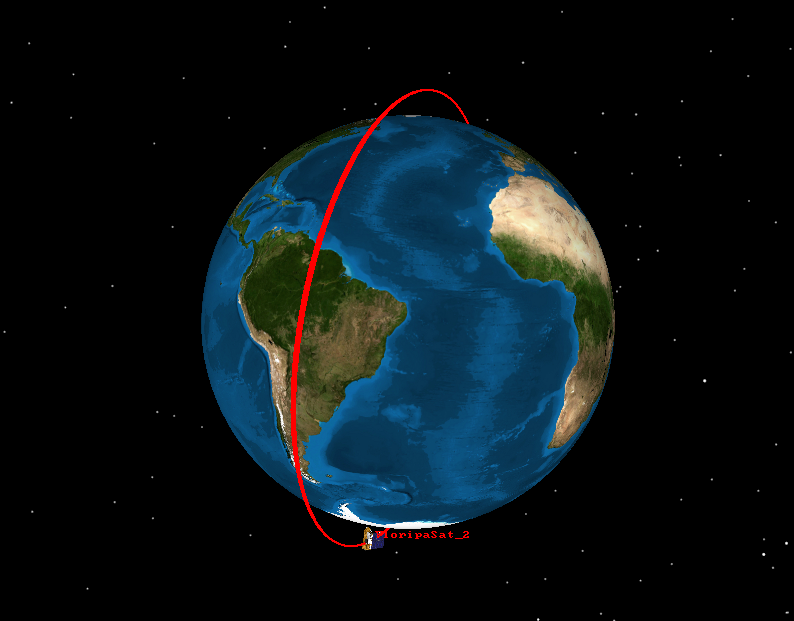
\includegraphics[width=0.6\textwidth]{figures/fsat2-gmat.png}
        \caption{Radio Occultation orbit simulation on GMAT.}
        \label{fig:fsat2-gmat}
    \end{center}
\end{figure}

\begin{figure}[!ht]
    \begin{center}
        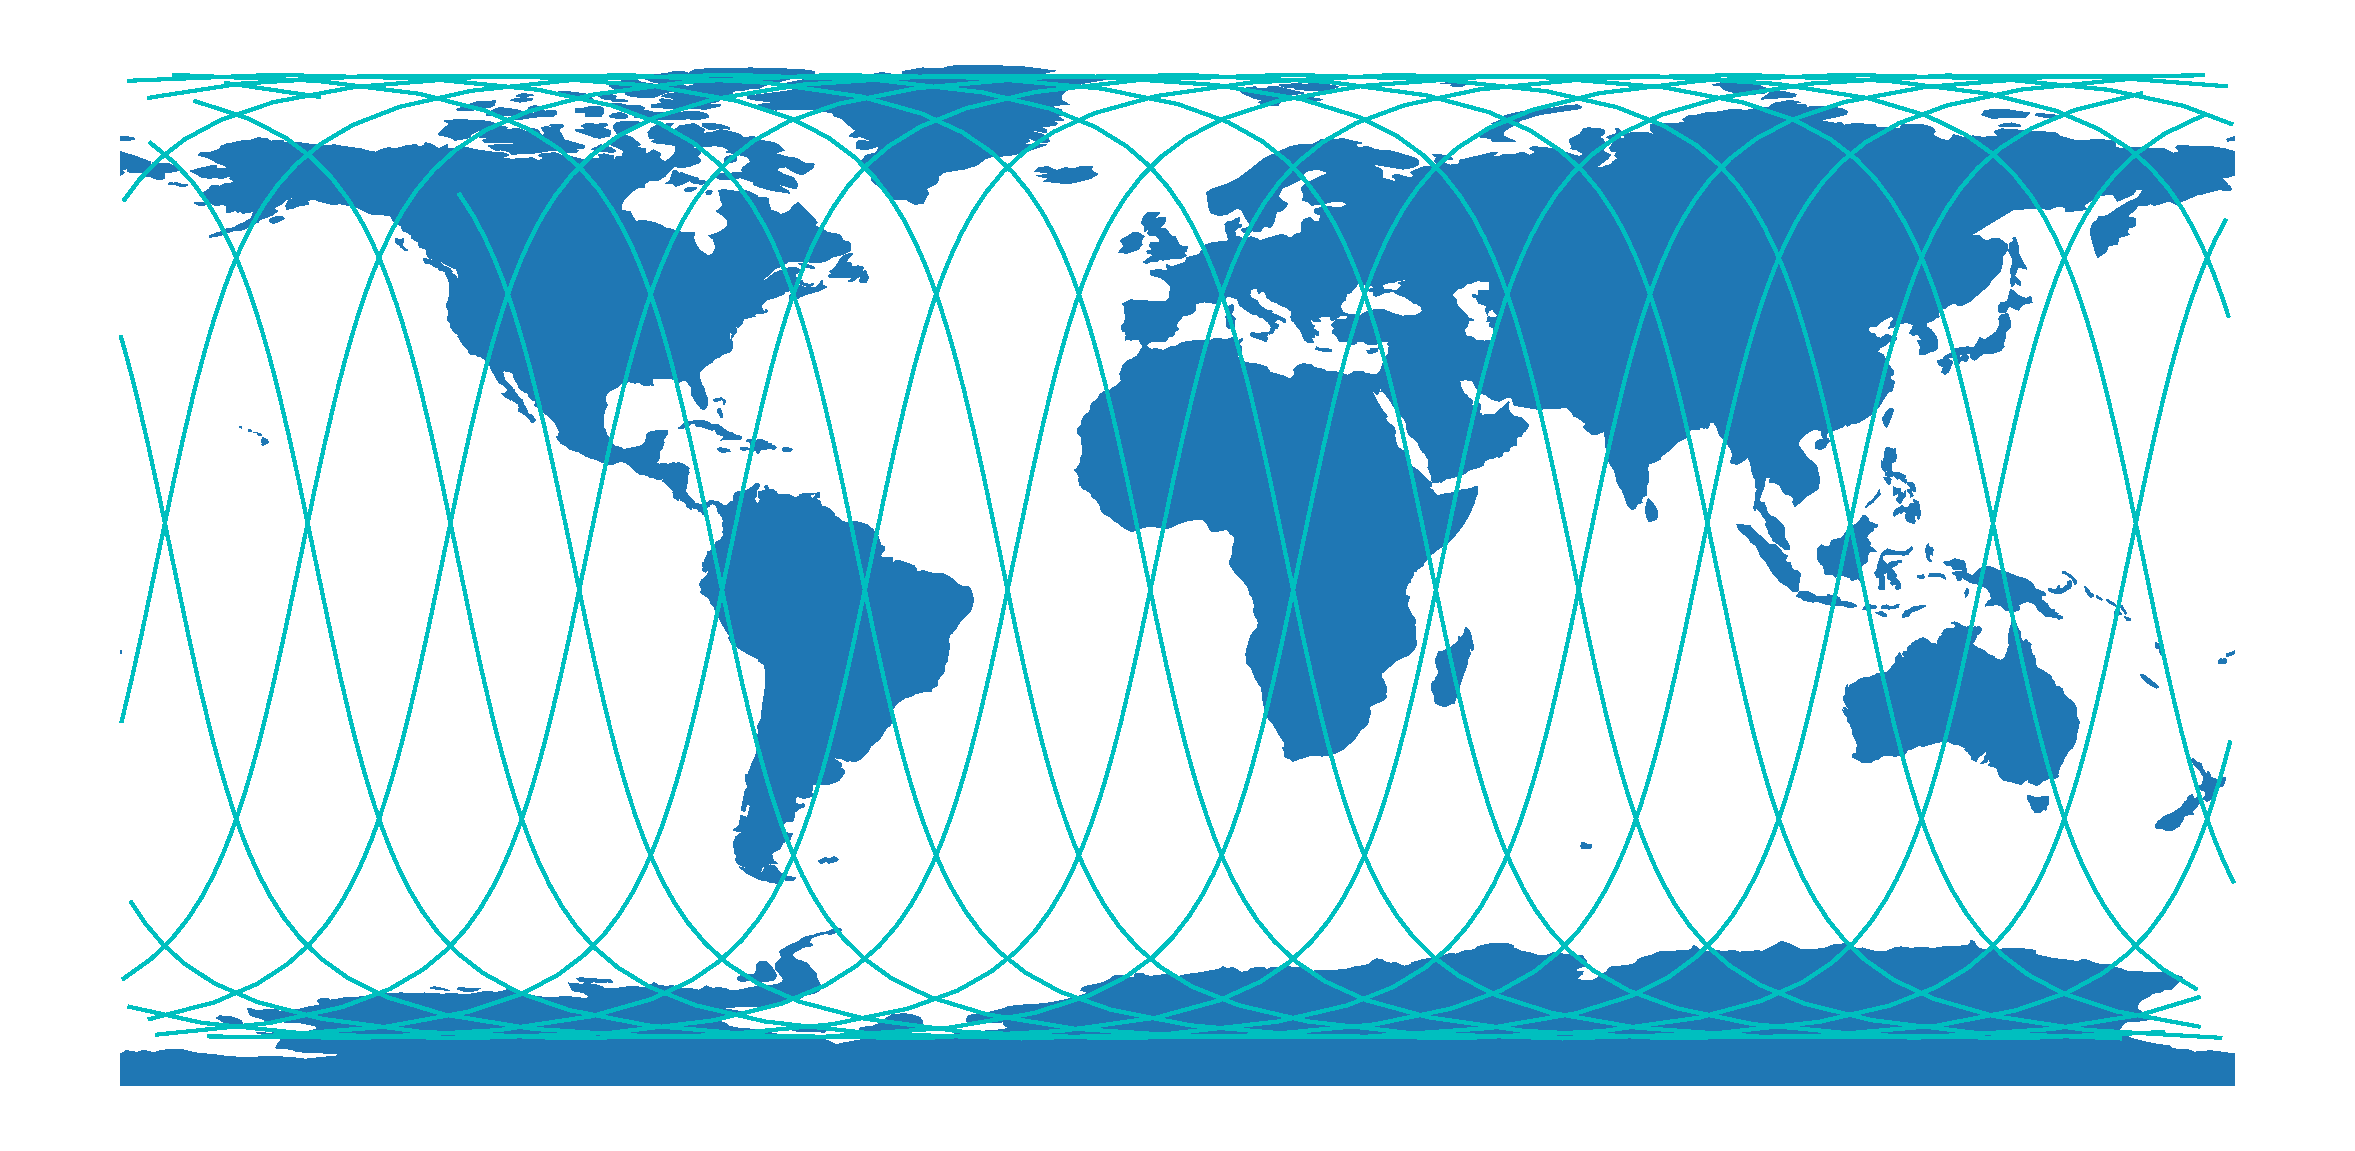
\includegraphics[width=\textwidth]{figures/fsat2-gmat-groundtrack.pdf}
        \caption{Radio Occultation simulated groundtrack.}
        \label{fig:fsat2-gmat-groundtrack}
    \end{center}
\end{figure}

The next sections present some analysis based on the results obtained from the simulations performed with SimCube.% executed on GMAT.

%The source files of the GMAT simulation are available in \cite{fsat2-mechanical}.

\subsection{ \textcolor{red}{TODO} Lifetime Analysis}

Considering the same parameters of Radio Occultation, but with an initial altitude of 550 km, the simulations on SimCube showed that the satellite decays approximately in 2183 days ($\cong$ 6 years), as can be seen in \autoref{fig:lifetime-analysis}.

\begin{figure}[!ht]
    \begin{center}
        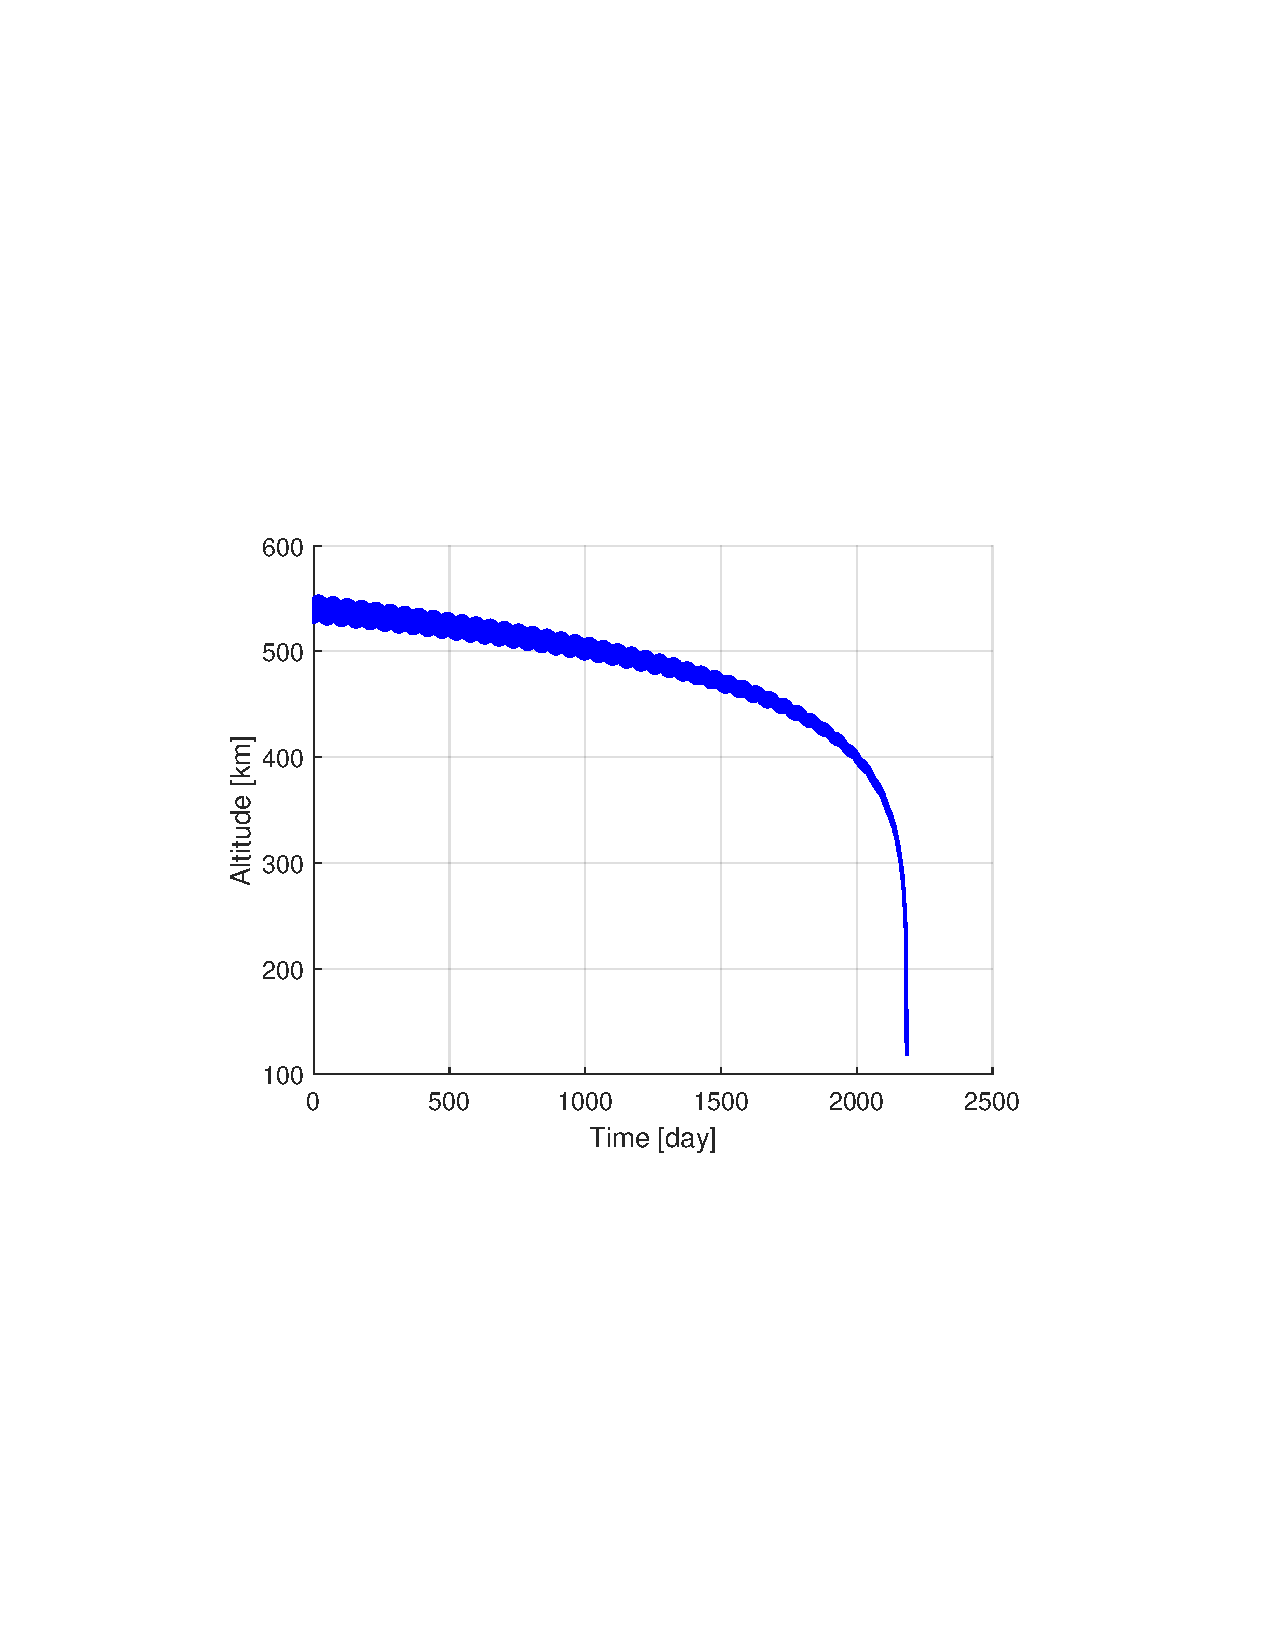
\includegraphics[trim=3.5cm 8cm 4.0cm 8cm,clip, width=0.8\textwidth]{curves/Altitude.pdf}
        \caption{Lifetime analysis.}
        \label{fig:lifetime-analysis}
    \end{center}
\end{figure}

\subsection{ \textcolor{red}{TODO} Ground Station Passes and Data Transfer Analysis}

Considering two ground stations, one at the SpaceLab installations in Florianópolis (27$^{\circ}$ 36' 00.9" S, 48$^{\circ}$ 31' 03.2" W) and other at the INPE/CRN installations in Natal (5$^{\circ}$ 50' 10.1" S, 35$^{\circ}$ 12' 27.5" W), both with a minimum elevation of 15$^{\circ}$, the results in \autoref{tab:grs-contacts-analysis}) were achieved. %during the simulations on GMAT .

\begin{table}[!h]
    \centering
    \begin{tabular}{lccc}
        \toprule[1.5pt]
        \textbf{Parameter} & \textbf{UFSC Station} & \textbf{INPE-RN Station} & \textbf{Unit} \\
        \midrule
        Minimum elevation to a valid contact    & 15    & 15    & $^{\circ}$ \\
        Number of contacts                      & 143   & 125   & - \\
        Minimum contract period                  & 24    & 34    & sec \\
        Maximum contact period                  & 395   & 394   & sec \\
        Average contact period                  & 303   & 298   & sec \\
        Total contact period                    & 43394 & 37205 & sec \\
        \bottomrule[1.5pt]
    \end{tabular}
    \caption{Ground station contacts analysis during the first 60 days of operation.}
    \label{tab:grs-contacts-analysis}
\end{table}

As seen from \autoref{tab:grs-contacts-analysis}, during the first 60 days of operation, considering the two main ground stations that will contact the satellite, the total contact period is 80599 seconds (43394 + 37205). With the data rate of the downlink/uplink as 4800 bps, this period will allow a data transfer of 48359400 bytes (or 46.12 M$_{i}$B) between Radio Occultation and the Earth. Using the satellite's lifetime from the previous analysis (2000 days), and an average data transfer per day of 805990 bits, the total theoretical raw data transfer during the whole operation of the satellite will be approximately 1.5 G$_{i}$B.

These values can be even more significant if a smaller minimum elevation is considered, or with more ground stations in other locations.

\section{ \textcolor{red}{TODO} Mass Budget} \label{mass-budget}

The mass budget of the satellite can be seen in \autoref{tab:mass-budget}.

\begin{table}[!h]
    \centering
    \begin{tabular}{llc}
        \toprule[1.5pt]
        \textbf{Subsystem} & \textbf{Model} & \textbf{Mass [g]} \\
        \midrule
        OBDH                        & SpaceLab OBDH 2.0             & 53 \\
        TTC                         & SpaceLab TTC 2.0              & 52 \\
        EPS                         & SpaceLab EPS 2.0              & 80 \\
        Battery                     & SpaceLab Battery Module 4C    & 235 \\
        Antenna                     & ISISpace AntS                 & 89 \\
        ACS                         & SpaceLab Passive ACS 2U       & 100 (TBC) \\
        Payload                     & INPE-RN EDC                   & 75 ($\times$2) \\
        Radiation instrument            & SpaceLab Payload X            & 75 (TBC) \\
        Interface                   & SpaceLab Interface Boards     & 40 \\
        PC-104 Adapter              & SpaceLab PC-104 Adapter       & 50 (TBC) \\
        Solar Panel                 & Orbital Custom Solar Panel    & 266 \\
        Shields                     & 3 mm aluminum sheets          & 590 (TBC) \\
        Structure                   & Usiped Custom 2U Structure    & 206 \\
        Cables                      & -                             & 200 \\
        Others                      & -                             & 100 \\
        \midrule
        Total                       & -                             & \textbf{2211} \\
        Max. CubeSat 2U             & -                             & 2666 \\
        Margin                      & -                             & 455 \\
        \bottomrule[1.5pt]
    \end{tabular}
    \caption{Mass budget of the satellite.}
    \label{tab:mass-budget}
\end{table}

According to the CubeSat standard \cite{cds}, the maximum mass of each unit must be 1.33 kg. As the Radio Occultation is a 2U CubeSat, the maximum allowed mass of the project is 2.66 kg. Considering the weight of each subsystem presented in \autoref{tab:mass-budget}, the current total mass of the object is below the maximum allowed, with a margin of 16 \%.

\section{ \textcolor{red}{TODO} Power Budget} \label{power-budget}

According to section 10.3 of \cite{larson2005}, the power budget of a satellite can be determined through three steps:

\begin{enumerate}
    \item Prepare operating power budget
    \item Size the battery
    \item Estimate power degradation over mission life
\end{enumerate}

\subsection{ \textcolor{red}{TODO} Input Power}

Simulations of the energy input to the solar panels along some orbits can be seen in the \autoref{fig:sp_sim_power} graph. Two extreme orbit scenarios, without and with maximum eclipse, were tested. The figures show the power generated on each side of the CubeSat, as well the total and average values.

\begin{figure}[!htb]
    \begin{center}
        \subfigure[Maximum eclipse.\label{fig:max_eclipse}]
        {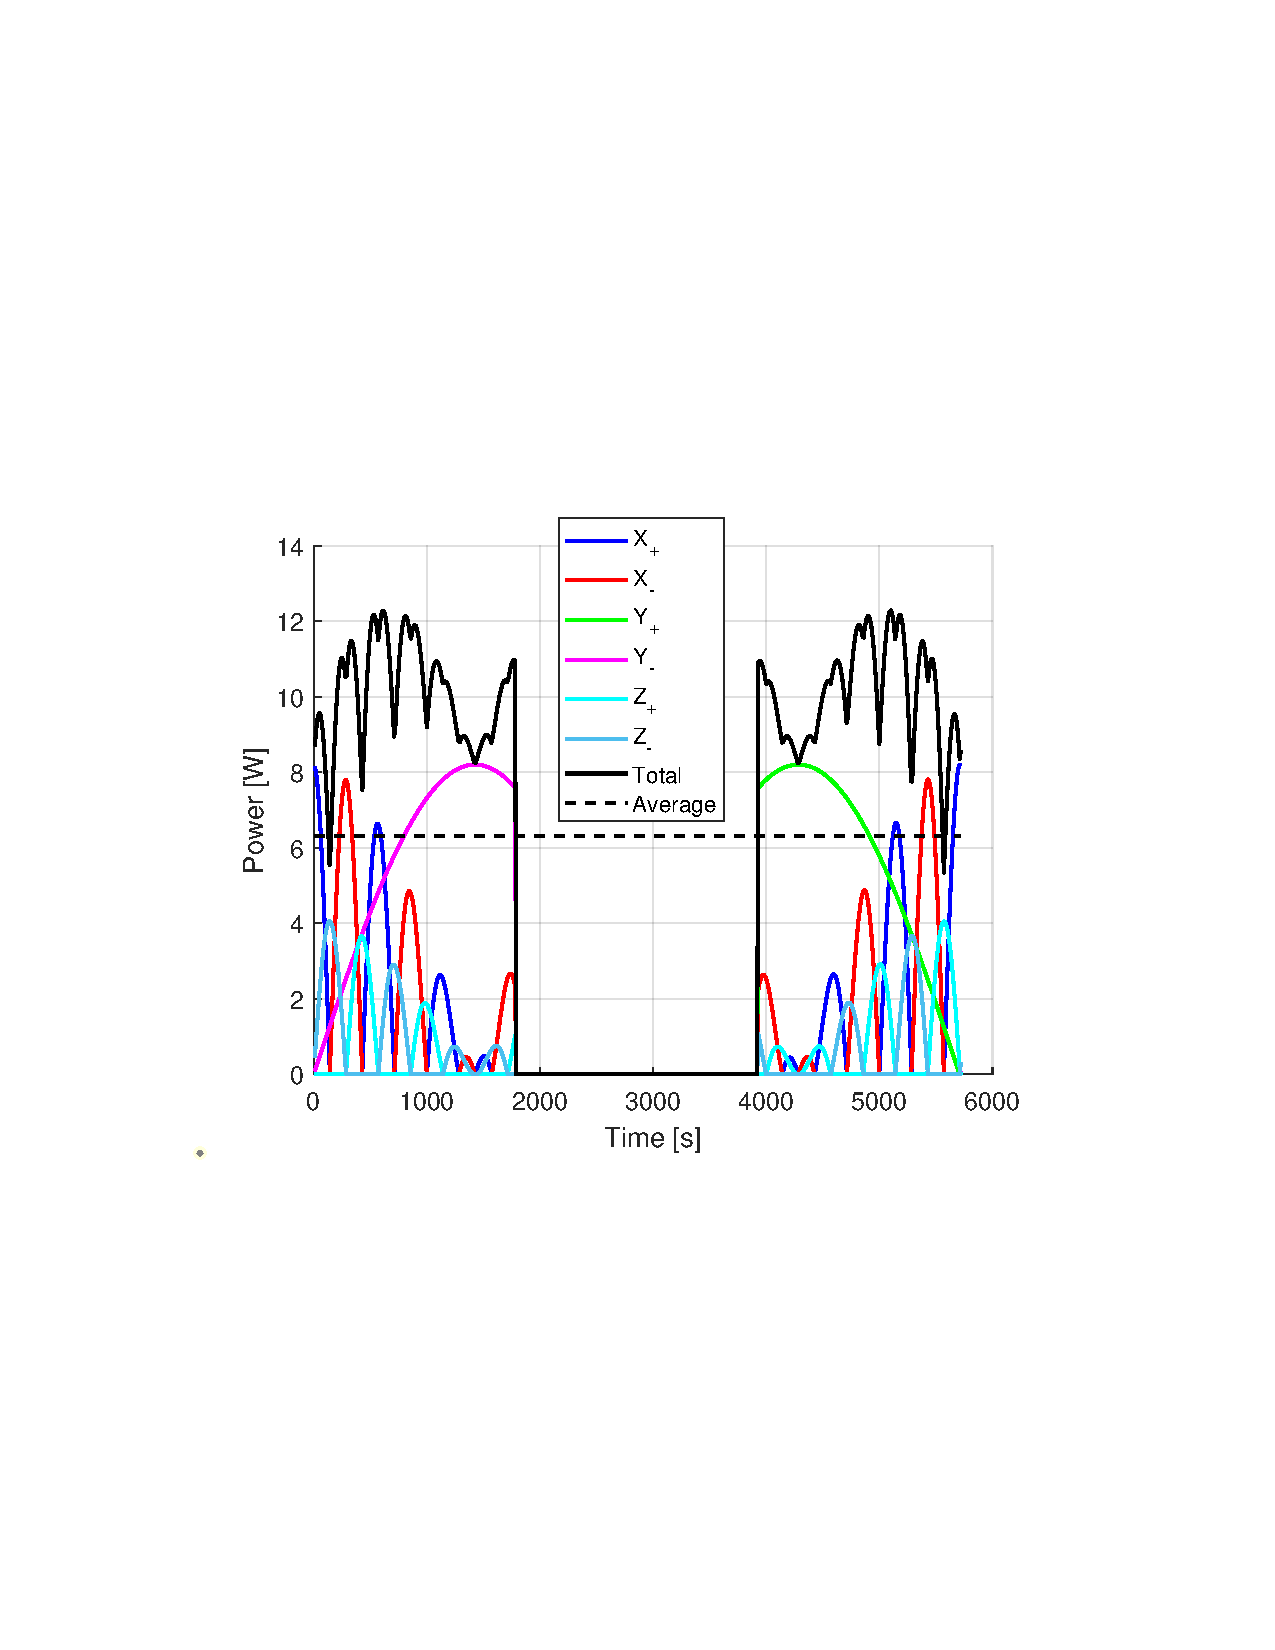
\includegraphics[trim=4cm 8.5cm 4cm 8.5cm, clip, width=0.45\textwidth]{curves/GOLDS_com_eclipse.pdf}}
        ~
        \subfigure[Without eclipse.\label{fig:without_eclipse}]
        {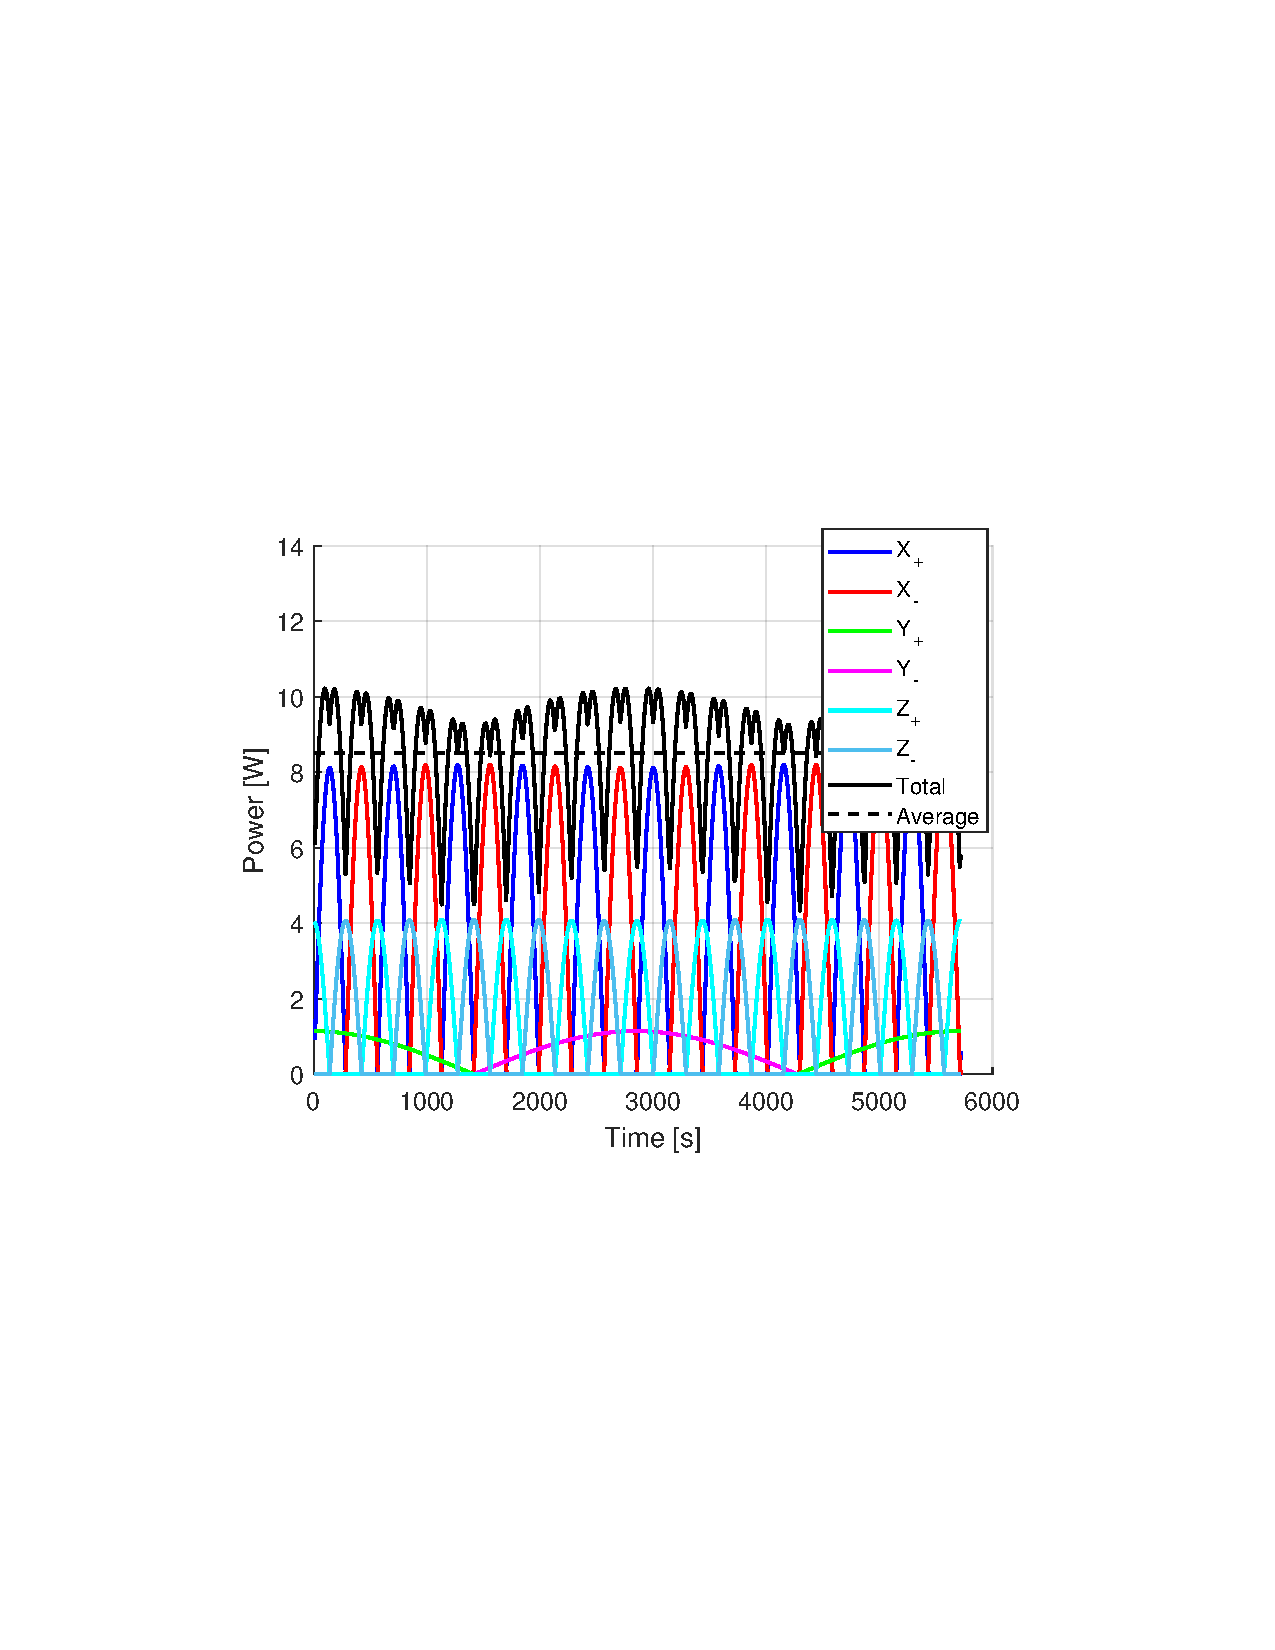
\includegraphics[trim=4cm 8.5cm 4cm 8.5cm, clip, width=0.45\textwidth]{curves/GOLDS_sem_eclipse.pdf}}
        \caption{Simulated input power of the solar panels.}
        \label{fig:sp_sim_power}
    \end{center}
\end{figure}

From these simulations, the results in \autoref{tab:power-simulations} were obtained:

\begin{table}[!htb]
    \centering
    \begin{tabular}{lcc}
        \toprule[1.5pt]
        \textbf{Parameter} & \textbf{Maximum eclipse} & \textbf{Without eclipse} \\    \midrule
        Peak power & 12282.7 mW & 10217.2 mW\\
        Average power (total orbit) & 6306.9 mW & 8519.6 mW \\
        Average (sunlight) & 10048.9 mW & 8519.6 mW\\
        Orbit period & 5720 s & 5720 s \\
        Sun light period &  3590 s & 5720 s\\
        Eclipse period & 2130 s & 0 s \\
        \bottomrule[1.5pt]
    \end{tabular}
    \caption{Results for the power input.}
    \label{tab:power-simulations}
\end{table}


\subsection{ \textcolor{red}{TODO} Operating Power Budget}

Typical operating voltages and current and power ranges consumed by each satellite subsystem are presented in \autoref{tab:power-requirements}.

\begin{table}[!h]
    \centering
    \begin{tabular}{lccccc}
        \toprule[1.5pt]
        \multirow{2}{*}{\textbf{Module}} & \multirow{2}{*}{\textbf{Voltage [V]}}    & \multicolumn{2}{c}{\textbf{Current [mA]}} & \multicolumn{2}{c}{\textbf{Power [mW]}} \\
                                         &                                          & \textbf{Min.} & \textbf{Max.}             & \textbf{Min.} & \textbf{Max.} \\
        \midrule
        OBDH                & 3.3   & 35    & 200   & 115   & 660 \\
        TTC ($\mu$C)        & 3.3   & 40    & 40    & 132   & 132 \\
        TTC (radio module)  & 5     & 10    & 650   & 33    & 3250 \\
        EPS (digital part)  & 7.4   & 50    & 260   & 165   & 858 \\
        EPS (heater)        & 7.4   & 675   & 675   & 5000  & 5000 \\
        Antenna module      & 3.3   & 60    & 550   & 200   & 1800 \\
        Payload EDC         & 5     & 250   & 250   & 1250  & 1250 \\
        Radiation instrument           & 5     & TBD   & TBD   & TBD   & TBD \\
        \bottomrule[1.5pt]
    \end{tabular}
    \caption{Power requirements of the subsystems and payloads of the satellite.}
    \label{tab:power-requirements}
\end{table}

Using the information presented in \autoref{tab:power-requirements}, and the activation periods defined for each module (the duty cycle), we arrive at the average satellite consumption present in \autoref{tab:power-consumption}.

\begin{table}[!h]
    \centering
    \begin{tabular}{lccccc}
        \toprule[1.5pt]
        \textbf{Module} & \textbf{Duty Cycle [\%]}    & \textbf{Power [mW]} \\
        \midrule
        OBDH                    & 100   & 115 \\
        TTC (radio 1 RX)        & 95    & 65 \\
        TTC (radio 1 TX)        & 5     & 3250 \\
        TTC (radio 2 RX)        & 95    & 65 \\
        TTC (radio 2 TX)        & 5     & 3250 \\
        EPS                     & 100   & 320 \\
        BAT (idle)              & 90    & 0 \\
        BAT (heater full)       & 10    & 5000 \\
        Antenna (deployment)    & 0     & 1800 \\
        Antenna (deployed)      & 100   & 35 \\
        Payload EDC             & 100   & 1250 \\
        Radiation instrument        & 0     & 1000 \\
        \cmidrule{2-3}
        Satellite               & \multicolumn{2}{c}{$\cong$ 2668} \\
        \bottomrule[1.5pt]
    \end{tabular}
    \caption{Power consumption of the subsystems and payloads of the satellite.}
    \label{tab:power-consumption}
\end{table}

The duty cycles of \autoref{tab:power-consumption} were defined according to the following assumptions:

\begin{itemize}
    \item One of the EDC payload is always off (cold redundancy).
    \item The Radiation instrument is turned on just during limited periods and only with telecommands.
\end{itemize}

As can be seen from \autoref{fig:sp_sim_power} and \autoref{tab:power-consumption}, there is a slight positive margin of \textbf{76.9 mW} in the power budget.

\subsection{ \textcolor{red}{TODO} Battery Sizing}

As described in \cite{larson2005}, the battery sizing of a satellite can be made by following the steps below:

\begin{enumerate}
    \item Estimate power level that the battery must supply
    \item Compute discharge cycle duration, charge cycle duration, and numbers of charge-discharge cycles
    \item Select depth of discharge
    \item Select charge rate
    \item Compute battery recharge power
\end{enumerate}

The power level that the battery must supply is the total power consumption of the satellite and is available in \autoref{tab:power-consumption}.

The discharge and charge cycle duration can be obtained from \autoref{fig:sp_sim_power}. The discharge duration is approximately 35.3 min (or 0.5889 h), and the charge cycle duration is 61.83 min (or 1.031 h). This is considering a single complete orbit.

The depth of discharge (DoD\nomenclature{\textbf{DoD}}{\textit{Depth of Discharge.}}) can be obtained using the \autoref{eq:dod-equation}.

\begin{equation} \label{eq:dod-equation}
    DoD = \frac{D_{i} \cdot D_{t}}{C} \cdot 100\ \%
\end{equation}

Where:

\begin{itemize}
    \item $D_{i}$: Discharge rate
    \item $D_{t}$: Discharge period
    \item $C$: Battery capacity
\end{itemize}

As the battery cells are already selected (5000 mAh in total, as described in \autoref{ssec:battery-module}), the current DoD is computed in \autoref{eq:dod-value}.

\begin{equation} \label{eq:dod-value}
    DoD = \frac{2668\ mW \cdot 0.5889\ h}{18500\ mWh} \cdot 100 \cong \mathbf{8.5\ \%}
\end{equation}

The charge rate can be estimated from the power input of the solar panels when the satellite is in sunlight. As presented before, the simulation results estimate the power input as 4315.6 mW. Considering the charge time as 61.83 min (or 1.031 h), the input energy is 4450 mWh. From \autoref{tab:power-consumption}, the power consumption of the satellite at sunlight is 2169 mW (or 2236 mWh considering the sunlight period). This way, energy input at sunlight is obtained in \autoref{eq:energy-input-sun-light}.

\begin{equation} \label{eq:energy-input-sun-light}
    4450 - 2236 = 2214\ mWh
\end{equation}

From the DoD calculation, the energy consumption during the eclipse is 1571 mWh. This way, the energy margin of the battery becomes positive ($2214 - 1571 = 643 mWh$), as expected from the power budget results.

All results from the battery sizing are available in \autoref{tab:battery-sizing-results}.

\begin{table}[!h]
    \centering
    \begin{tabular}{lcc}
        \toprule[1.5pt]
        \textbf{Parameter} & \textbf{Value}    & \textbf{Unit} \\
        \midrule
        Battery capacity                & 18500  & mWh \\
        Energy consumption on sunlight & 2169   & mWh \\
        Energy consumption on eclipse   & 1571   & mWh \\
        Sunlight duration              & 1.031  & h \\
        Eclipse duration                & 0.5889 & h \\
        Depth of Discharge (DoD)        & 8.5    & \% \\
        Total battery energy margin     & 643    & mWh \\
        \bottomrule[1.5pt]
    \end{tabular}
    \caption{Battery sizing results.}
    \label{tab:battery-sizing-results}
\end{table}

From the results, the battery sizing is well suited for the current satellite configuration and the planned behavior.

\subsection{ \textcolor{red}{TODO} Power Degradation Over Mission Life}

Two major events along the satellite operation should be considered in the power degradation analysis:

\begin{enumerate}
    \item Solar panels degradation
    \item Battery degradation
\end{enumerate}

From \cite{larson2005}, 5 \% per year is a usual number for the solar panels' degradation, in other words, the general efficiency of the solar panels decays at a rate of 5 \% per year of operation.% Also, \cite{larson2005} defines the battery degradation (or aging )as XX \% per year.

%A partial discharge reduces stress and prolongs battery life, so does a partial charge. Elevated temperature and high currents also affect cycle life

\section{ \textcolor{red}{TODO} Link Budget}

The link budget of all satellite radio links is available in \autoref{tab:link-budget-results}.

\begin{table}[!h]
    \centering
    \begin{tabular}{L{0.3\textwidth}ccccc}
        \toprule[1.5pt]
        \textbf{Variable} & \textbf{Beacon} & \textbf{Downlink} & \textbf{Uplink} & \textbf{Uplink (Payload)} & \textbf{Unit}\\
        \midrule
        Altitude                        & 550           & 550           & 550           & 550           & km \\
        Elevation                       & 0             & 0             & 0             & 0             & $^{\circ}$ \\
        Frequency                       & 146           & 450           & 450           & 401.635       & MHz \\
        Modulation                      & GMSK          & GMSK          & GMSK          & BPSK          & - \\
        Protocol                        & NGHam         & NGHam         & NGHam         & SBCD          & - \\
        Transmit power                  & 30            & 30            & 44            & 30            & dBm \\
        Transmitter antenna gain        & 0             & 0             & 12            & 3             & dBi \\
        Receiver antenna gain           & 12            & 12            & 0             & 0             & dBi \\
        FSPL                            & 144.4         & 154.2         & 154.2         & 153.2         & dB \\
        Power at receiver               & -107.4        & -117.2        & -103.16        & -125.2        & dBm \\
        Receiver sensibility            & -134          & -134          & -126          & -128          & dBm \\
        System losses                   & 5             & 5             & 5             & 5             & dB \\
        Receiver noise temp.            & 361.7         & 361.7         & 361.7         & 361.7         & K \\
        Antenna noise temp.             & 300           & 300           & 300           & 300           & K \\
        System noise temp.              & 661.7         & 661.7         & 661.7         & 661.7         & K \\
        Data rate                       & 1200          & 9600          & 9600          & 400           & bps \\
        Received SNR                    & 32.22         & 13.41         & 27.41         & 19.17         & dB \\
        SNR required for $10^{-5}$ BER\footnotemark & 9.6           & 9.6           & 9.6           & 9.6           & dB \\
        Link margin                     & $\geq$ 22.62  & $\geq$ 3.812  & $\geq$ 17.81  & $\geq$ 9.57   & dB \\
        \bottomrule[1.5pt]
    \end{tabular}
    \caption{Link budget results.}
    \label{tab:link-budget-results}
\end{table}

\footnotetext{Without FEC\nomenclature{\textbf{FEC}}{\textit{Forward Error Correction.}}.}

As can be seen, considering the worst case for the estimated orbit, that is, with the satellite on the horizon and with an elevation of zero degrees, the margin of all links is positive with a considerable balance.

All equations and steps used to obtain the results of \autoref{tab:link-budget-results} are available in \autoref{anx:link-budget}.

    %
% design.tex
%
% Copyright (C) 2021 by SpaceLab.
%
% Radio Occultation Documentation
%
% This work is licensed under the Creative Commons Attribution-ShareAlike 4.0
% International License. To view a copy of this license,
% visit http://creativecommons.org/licenses/by-sa/4.0/.
%

%
% \brief Design description chapter.
%
% \author Gabriel Mariano Marcelino <gabriel.mm8@gmail.com>
%
% \institution Universidade Federal de Santa Catarina (UFSC)
%
% \version 0.9.0
%
% \date 2021/07/15
%

% \chapter{ \textcolor{red}{TODO} Design Description} \label{ch:design}
\chapter{ \textcolor{red}{TODO} Service Module Overview} \label{ch:design}

This section presents the design description of Radio Occultation.

\section{ \textcolor{red}{TODO} General Diagrams}

The CubeSat's subsystems are positioned in the 2U physical structure as exemplified in \autoref{fig:subsystems-positioning}. 
% An exploded 3D satellite view is shown in \autoref{fig:exploded-view}.

\begin{figure}[!htb]
    \begin{center}
        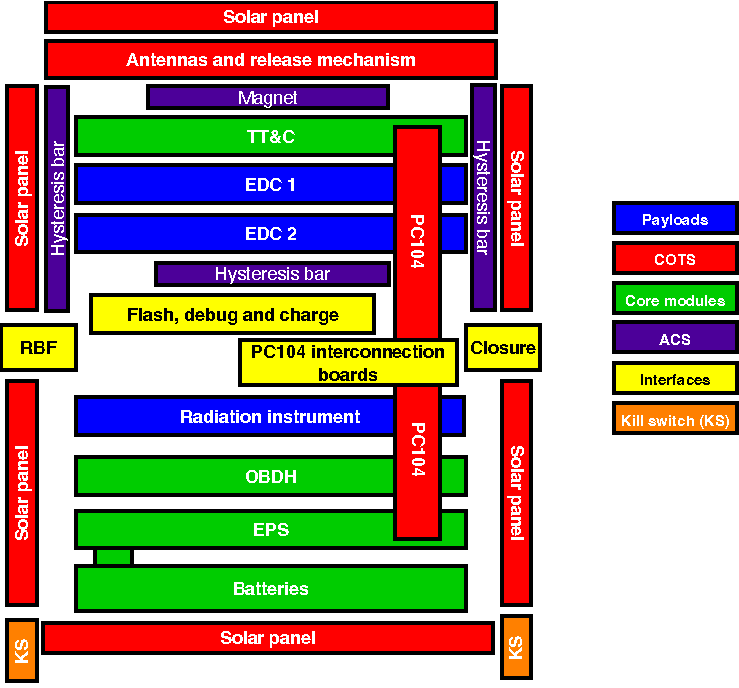
\includegraphics[width=0.7\textwidth]{figures/subsystems-positioning.pdf}
        \caption{Subsystems positioning.}
        \label{fig:subsystems-positioning}
    \end{center}
\end{figure}

\subsection{ \textcolor{red}{TODO} Power Diagram}

In \autoref{fig:power-diagram} is presented a block diagram showing the satellite's power buses.
The EPS module distributes these buses and has the ability to turn on and off some subsystems, while other modules also have direct control over some dc regulators\cite{eps2}.
The bus used for the antenna module is only active during its deployment. 
The current values shown are the maximum capability and not the nominal operating values; these are determined by the variable power generation of the solar panels as well as the loads present at a given time of the satellite's operation.
% TBD
% In \autoref{power-budget} the satellite's power consumption is shown in detail.

\begin{figure}[!htb]
    \begin{center}
        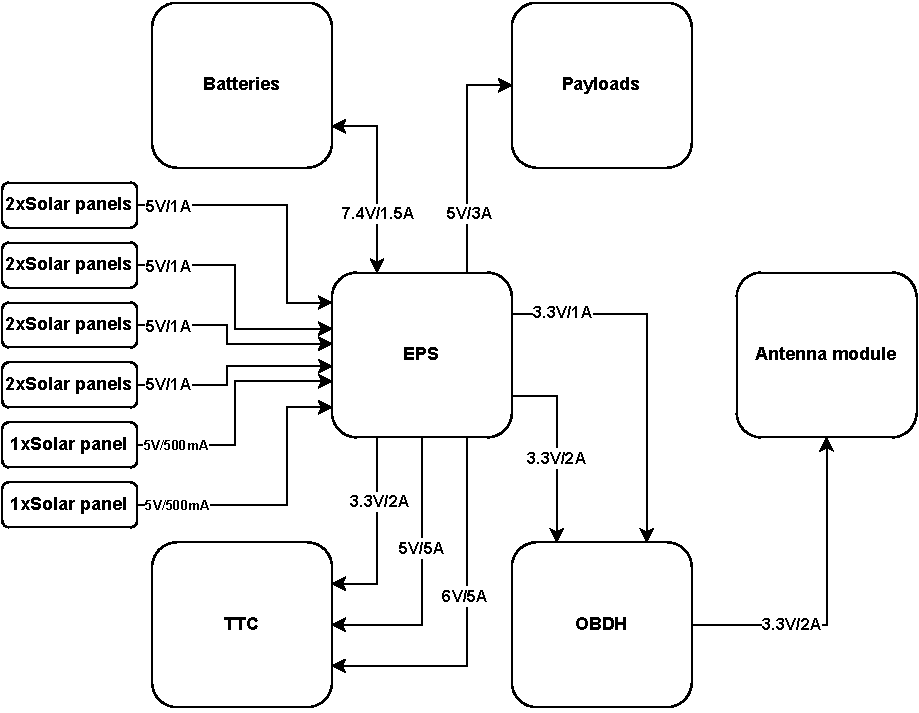
\includegraphics[width=\textwidth]{figures/power_diagram.pdf}
        \caption{Power diagram.}
        \label{fig:power-diagram}
    \end{center}
\end{figure}

%   TBD 
%   In \autoref{fig:datapath-diagram} there is a block diagram showing the satellite modules and the internal communication interfaces.

\subsection{ \textcolor{red}{TODO} Data Path Diagram}

The data path diagram is shown in \autoref{fig:data-path}.

\begin{figure}[!htb]
    \begin{center}
        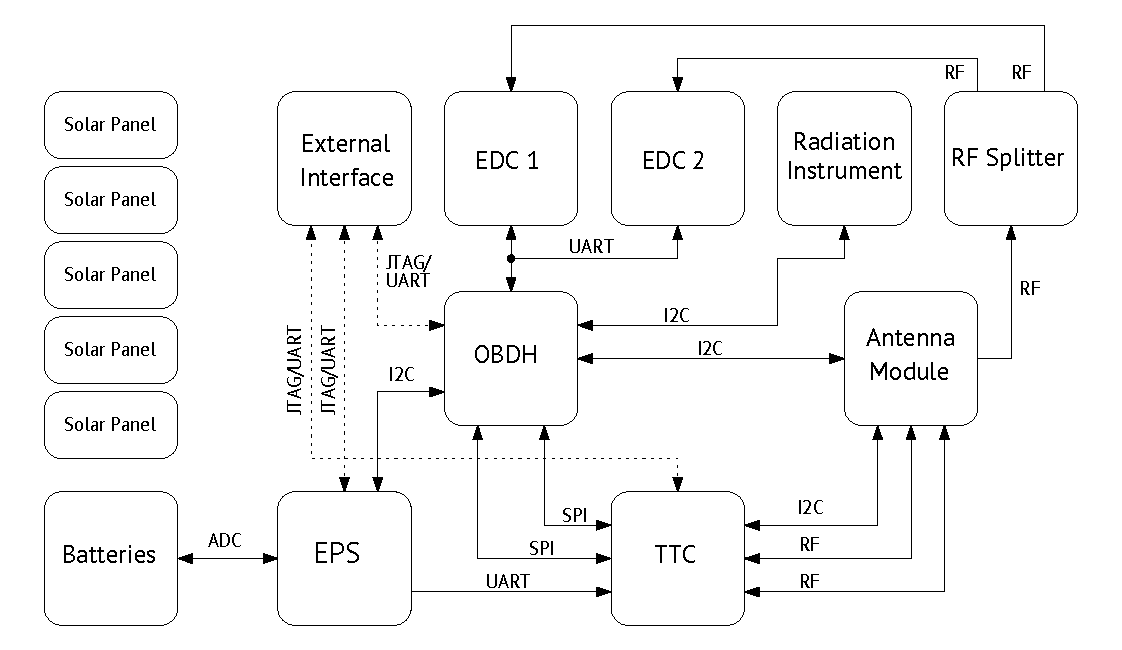
\includegraphics[width=\textwidth]{figures/data_path_diagram.pdf}
        \caption{Data path diagram.}
        \label{fig:data-path}
    \end{center}
\end{figure}

\subsection{ \textcolor{red}{TODO} Deployment Sequence}

The deployment sequence of the satellite is the routine to be executed just after the launch. The main objective of this operation is to deploy the antennas and prepare the satellite to start its normal operation.

After the satellite is ejected from the deployer, the kill switches enable the electric power and the three core modules to execute the boot sequence (EPS, OBDH and TTC). The EPS module is ready to operate when the boot finishes. The OBDH and the TTC modules waits for a determined period before starting the normal execution.

As the OBDH and the TTC have access to the antenna module, both subsystems can control the deployment of the antennas. Following the CDS\nomenclature{\textbf{CDS}}{\textit{CubeSat Design Specification.}} specifications \cite{cds}, all CubeSats must wait 30 minutes to deploy the antennas and 45 minutes to transmit any RF signal. This way, the OBDH waits 45 minutes to send the deployment command to the antenna module. As redundancy, the TTC waits 55 minutes to execute the same operation.

The \autoref{fig:deployment-flowchart} has a flowchart that illustrates the deployment sequence of the service modules.

\begin{figure}[!htb]
    \begin{center}
        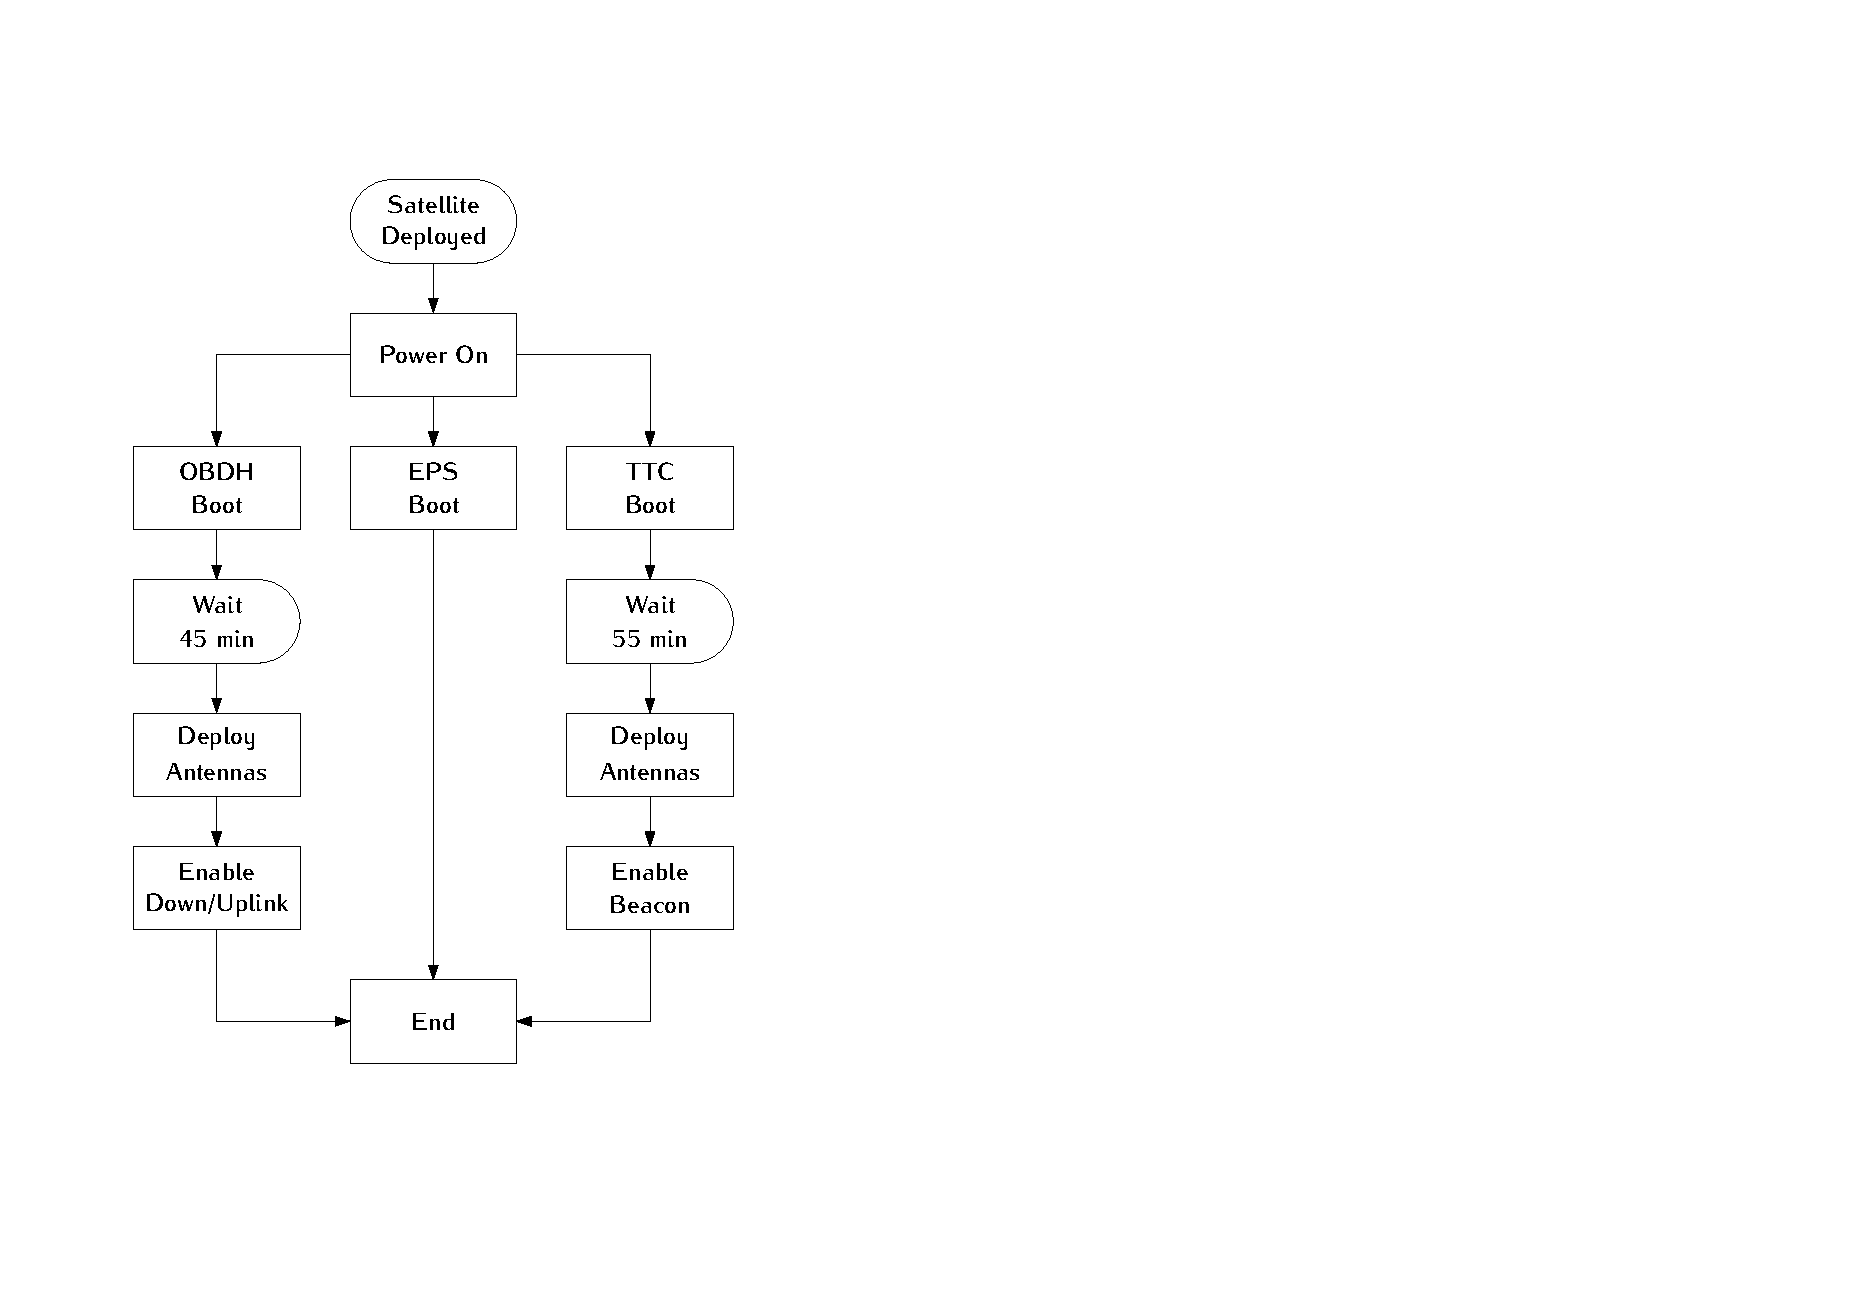
\includegraphics[width=0.5\textwidth]{figures/deployment-flowchart.pdf}
        \caption{Flowchart of the deployment sequence.}
        \label{fig:deployment-flowchart}
    \end{center}
\end{figure}

\subsection{ \textcolor{red}{TODO} Beacon Operation}

After the beacon microcontroller's boot sequence, the beacon's operation starts. The normal operation consists of reading the data from the EPS and the TTC modules, transmitting the valid data (EPS or TTC package, in this order of priority), waiting 60 seconds, and repeating this sequence. The \autoref{fig:beacon-flowchart} has a flowchart of this behavior.

\begin{figure}[!htb]
    \begin{center}
        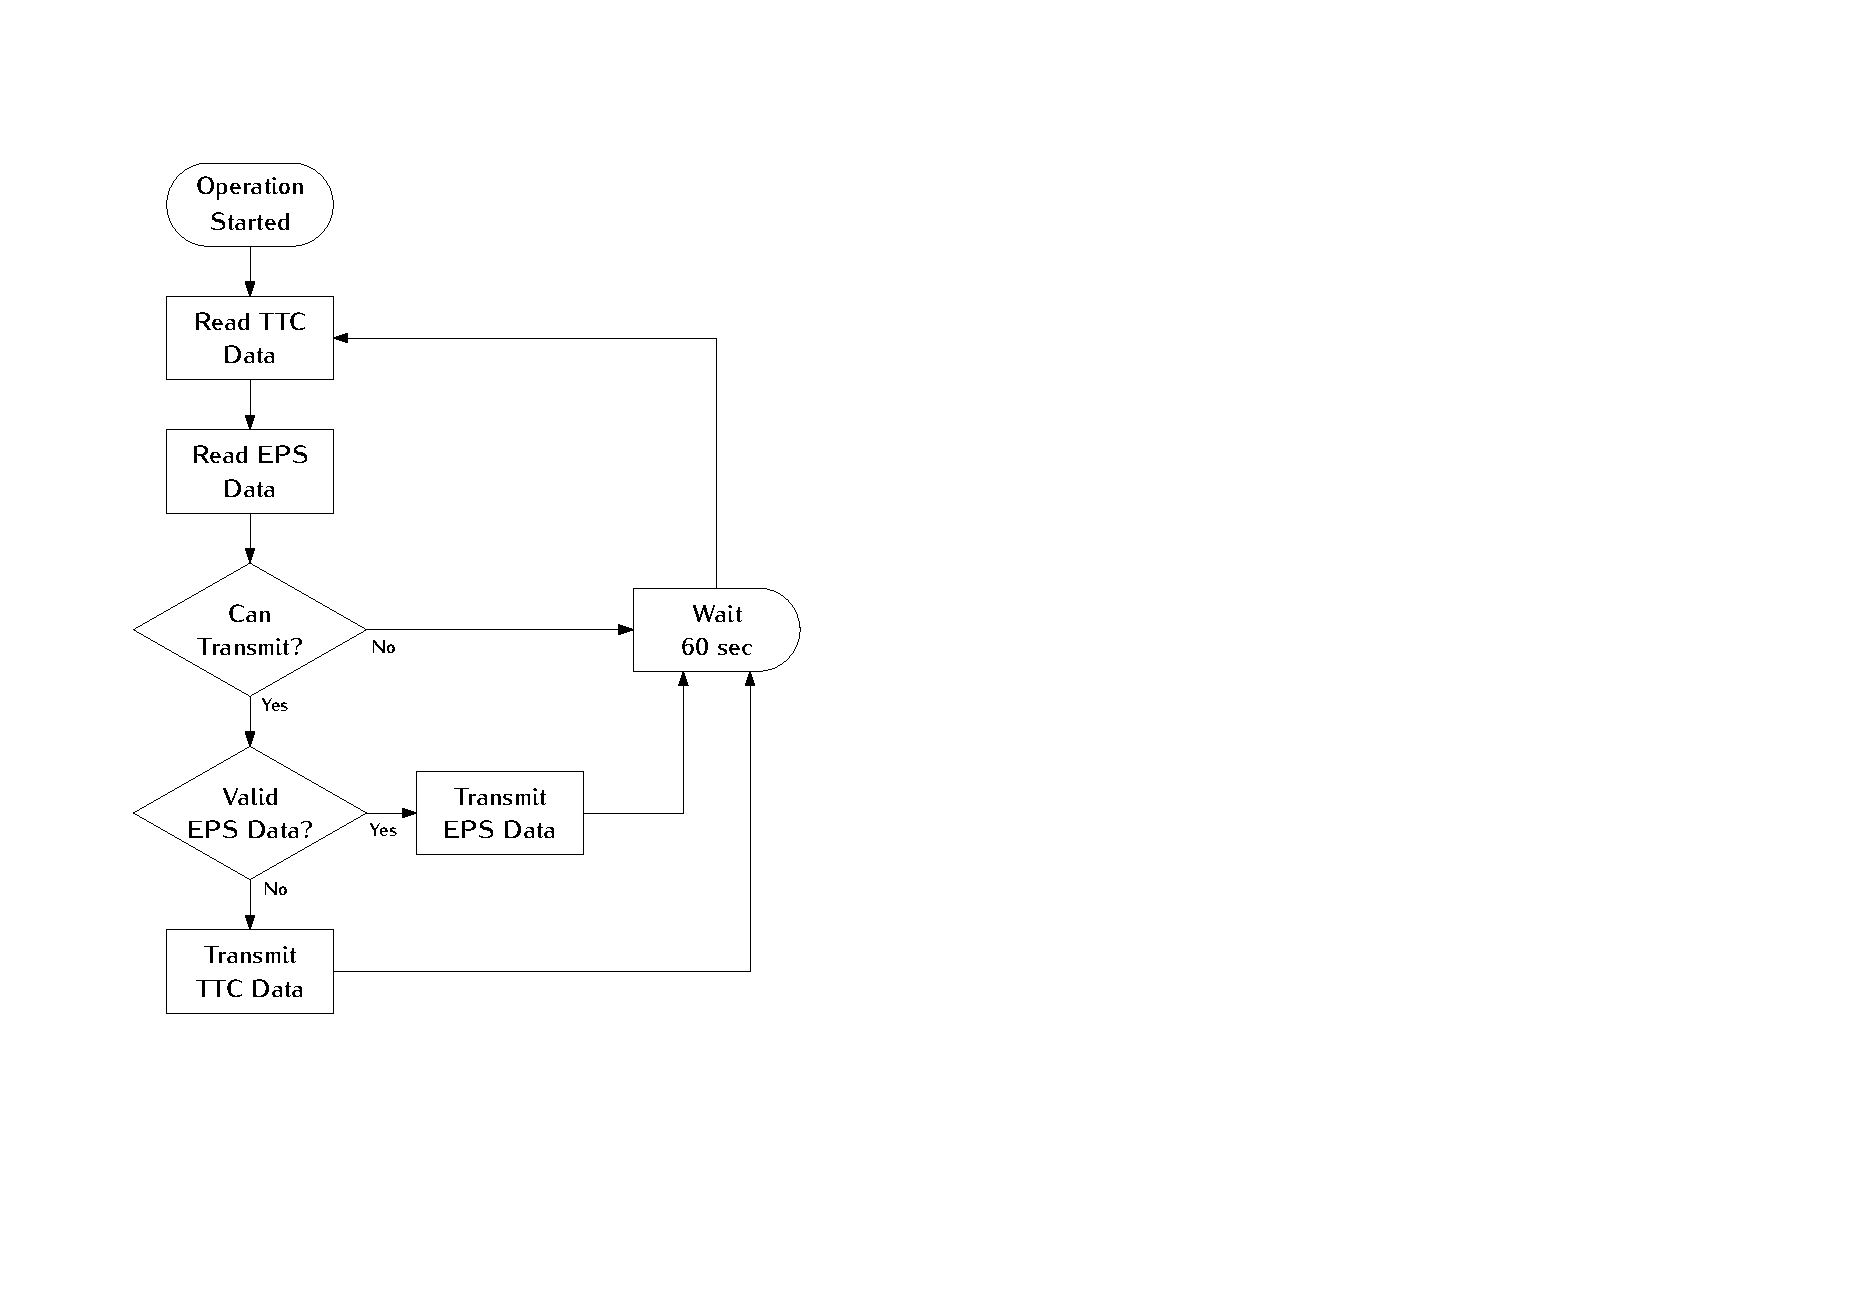
\includegraphics[width=0.55\textwidth]{figures/beacon-flowchart.pdf}
        \caption{Flowchart of the normal beacon operation.}
        \label{fig:beacon-flowchart}
    \end{center}
\end{figure}

\subsection{ \textcolor{red}{TODO} OBDH Operation}

After the boot sequence of the OBDH microcontroller, the operation of the OBDH starts. The regular operation consists of reading the housekeeping data from the EPS, TTC, payloads, antenna module, and the OBDH (its own housekeeping data), saving the read data on the non-volatile memory, and transmitting the housekeeping data of the satellite as a beacon. After that, it waits 60 seconds and checks if a new telecommand was received; if true, it processes the telecommand; if not, it does nothing. After this sequence, these steps start again. The \autoref{fig:obdh-flowchart} has a flowchart of this behavior.

\begin{figure}[!htb]
    \begin{center}
        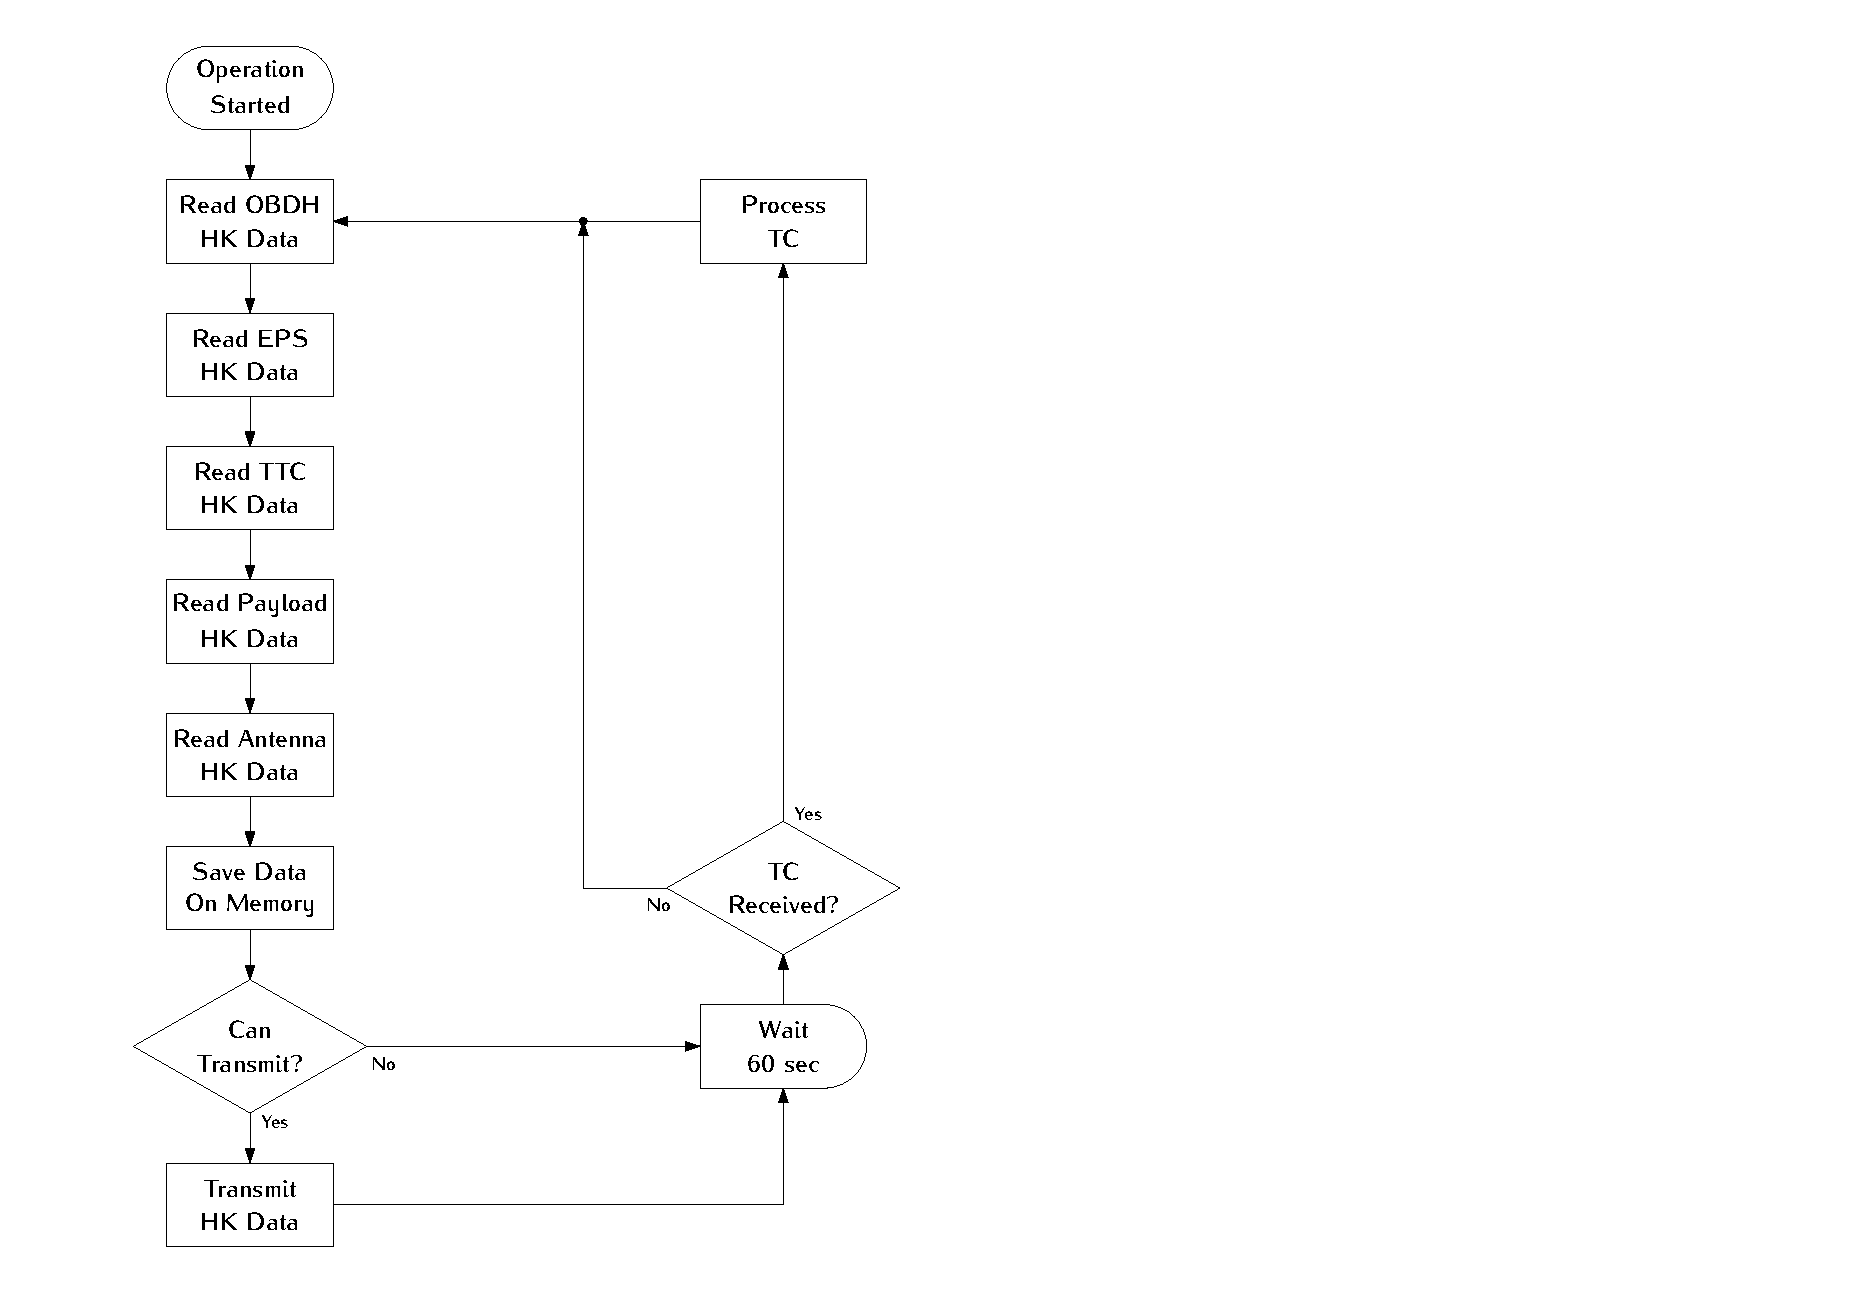
\includegraphics[width=0.63\textwidth]{figures/obdh-flowchart.pdf}
        \caption{Flowchart of the normal OBDH operation.}
        \label{fig:obdh-flowchart}
    \end{center}
\end{figure}

\subsubsection{Telecommand Processing}

Figure \autoref{fig:tc-flowchart} shows the telecommand processing flow.

\begin{figure}[!htb]
    \begin{center}
        \includegraphics[width=0.8\textwidth]{figures/tc-flowchart.pdf}
        \caption{Flowchart of telecommand processing.}
        \label{fig:tc-flowchart}
    \end{center}
\end{figure}

\subsection{ \textcolor{red}{TODO} EPS Operation}

The operation of the EPS microcontroller starts shortly after the release of the CubeSat in its orbit by the deployer.
In the first 60 minutes, the module operation consists of reading the housekeeping data from its sensors and managing the duty cycles of the MPPT and heaters.
When operational, the TTC and OBDH modules send separate periodic requests to the EPS for forwarding, the housekeeping data acquired.
The TTC receives a simplified version, while the OBDH receives a complete version of the data.
The \autoref{fig:eps-flowchart} has a flowchart of this behavior.

\begin{figure}[!htb]
    \begin{center}
        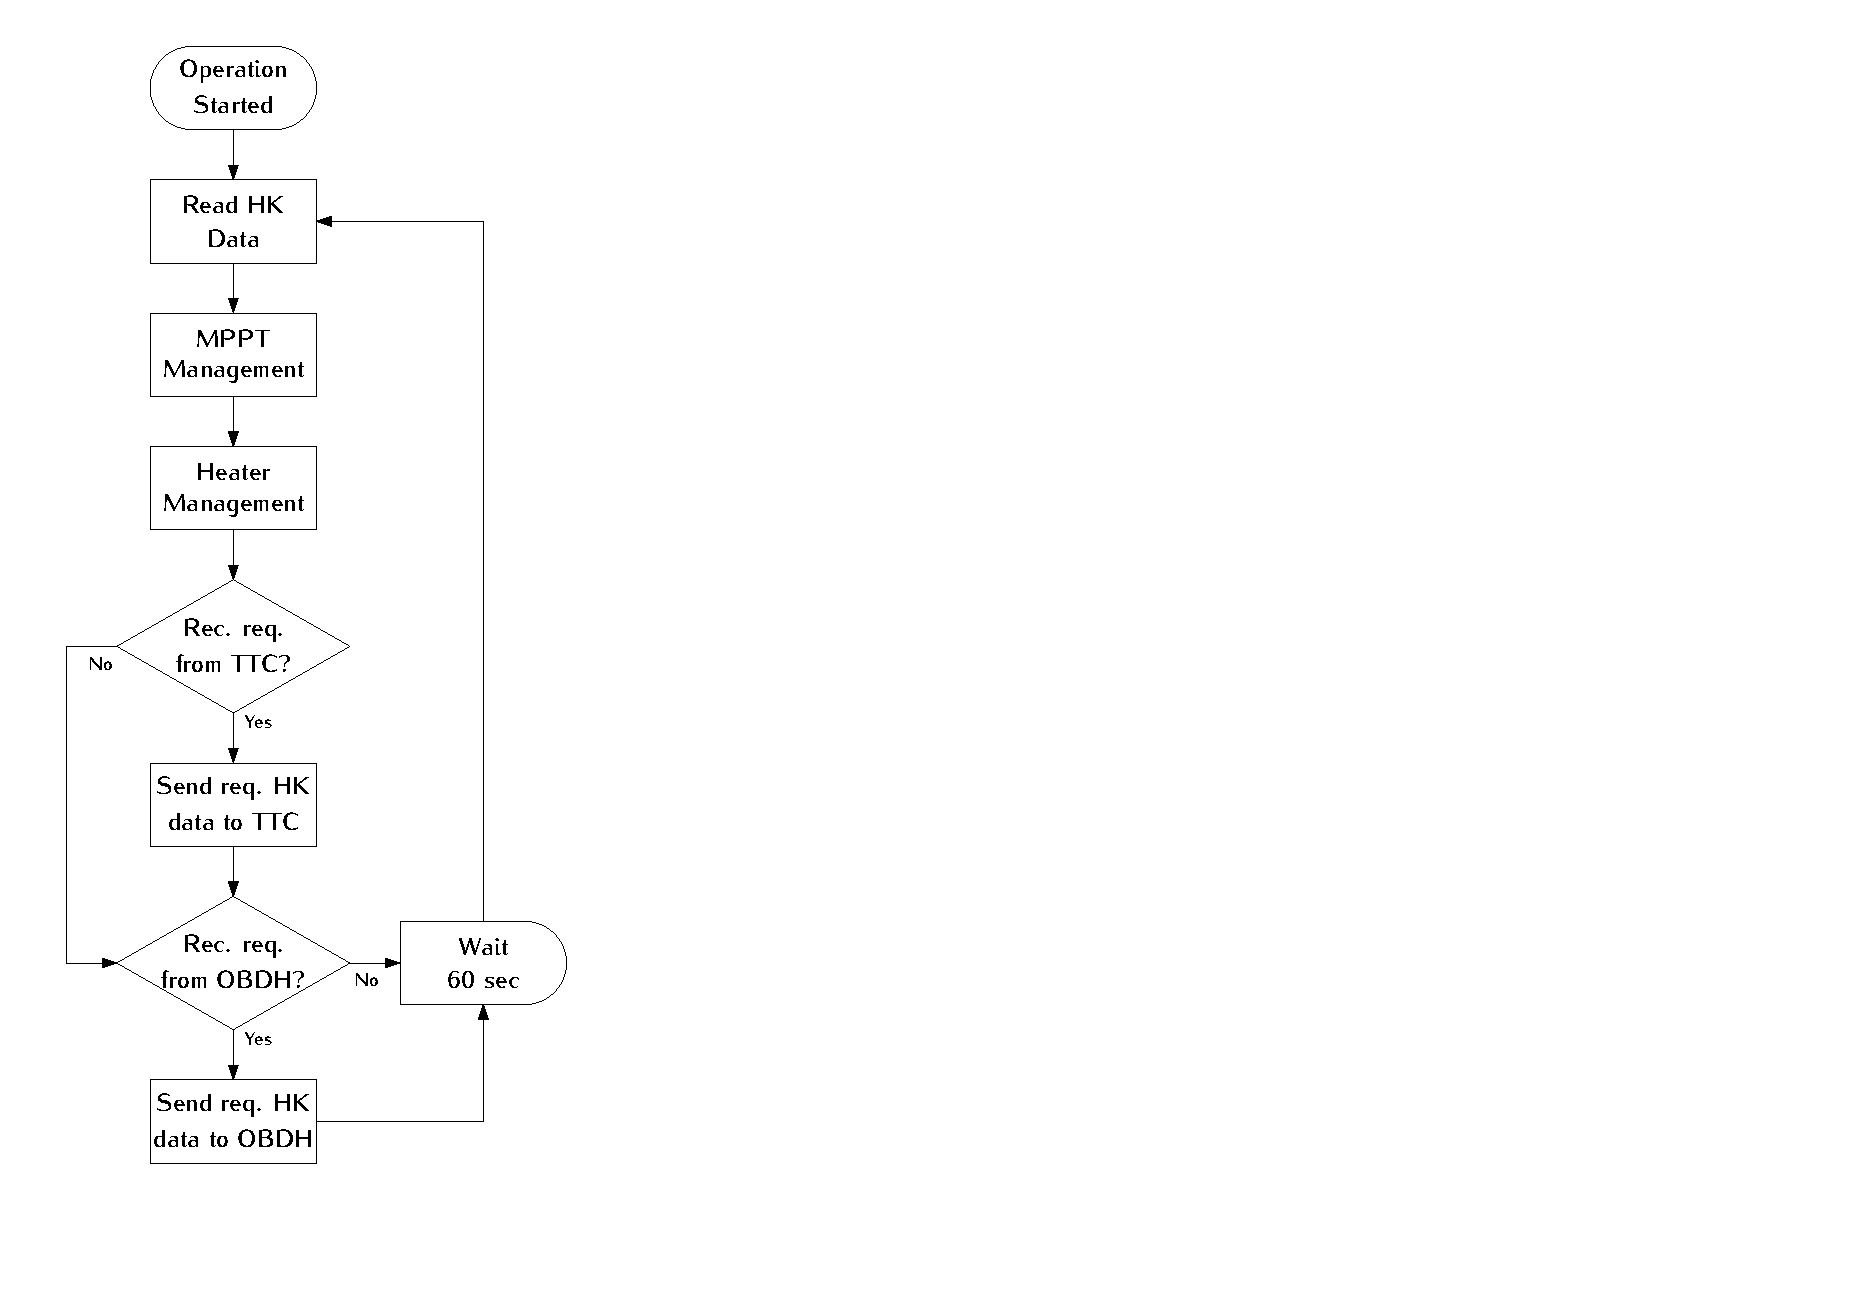
\includegraphics[width=0.45\textwidth]{figures/eps_flowchart.pdf}
        \caption{Flowchart of the normal EPS operation.}
        \label{fig:eps-flowchart}
    \end{center}
\end{figure}

%\section{ \textcolor{red}{TODO} General Behaviour}

%.

\section{ \textcolor{red}{TODO} Interface Data Sheet (IDS)}

\subsection{ \textcolor{red}{TODO} Interface}

To electrically connect all the satellite modules, a PC-104 bus standard is being used. This bus is composed by 104 lines disposed by four rows of 26 pins each (with a vertical and horizontal pitch of 2,54 mm).

Using the \autoref{fig:pc104-ref-diagram} as reference, all used positions and signals of the PC-104 bus are presented in \autoref{tab:pc104-pinout}. The \autoref{tab:pc104-signals} describes each signal and which modules are connected to them.

\begin{figure}[!htb]
    \begin{center}
        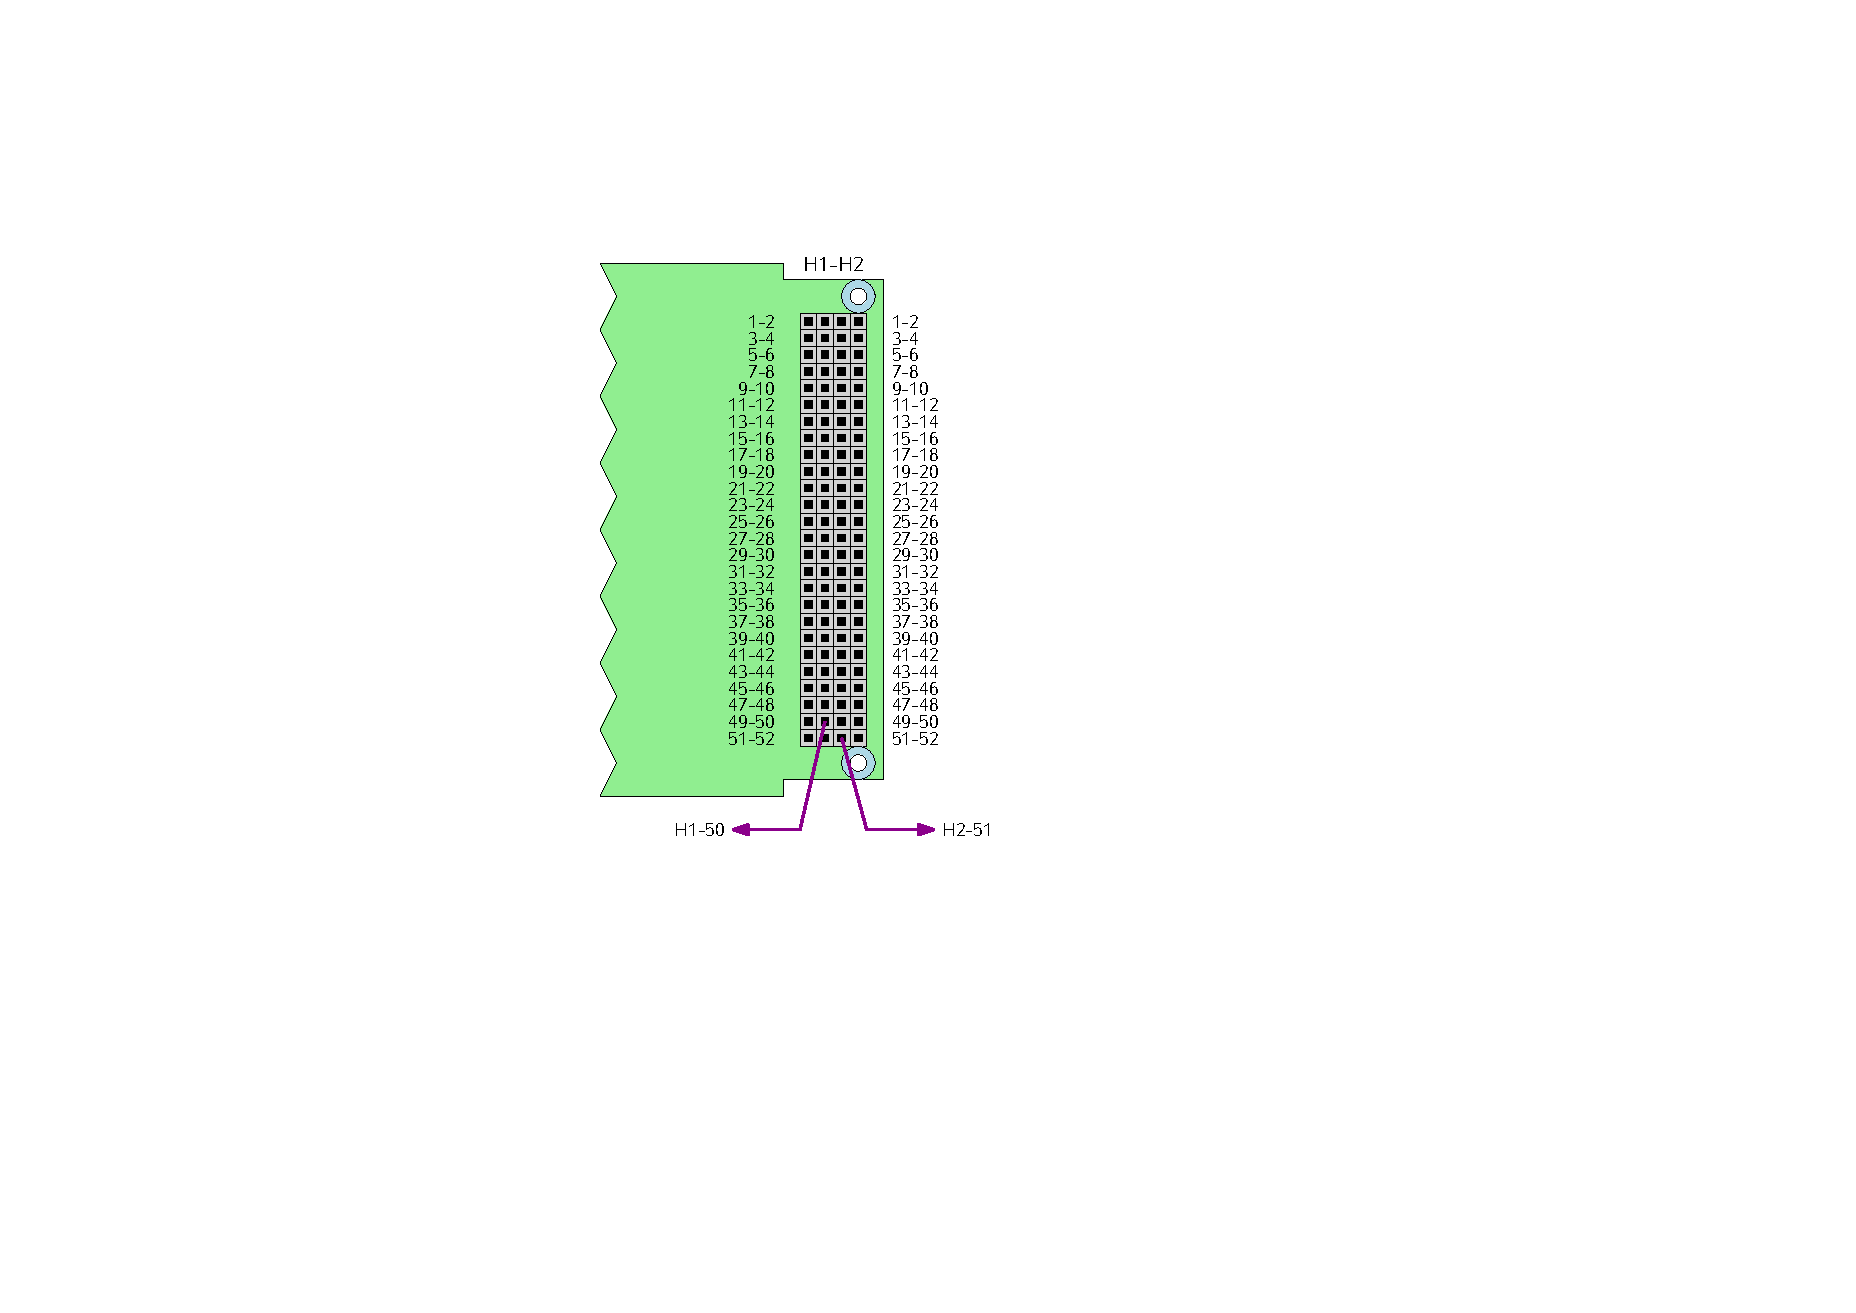
\includegraphics[width=0.5\textwidth]{figures/pc104-diagram}
        \caption{Reference diagram of the PC-104 bus (top view of a generic module).}
        \label{fig:pc104-ref-diagram}
    \end{center}
\end{figure}

\begin{table}[!h]
    \centering
    \begin{tabular}{cllll}
        \toprule[1.5pt]
        \textbf{Pin Row}   & \textbf{H1 Odd}  & \textbf{H1 Even} & \textbf{H2 Odd} & \textbf{H2 Even} \\
        \midrule
        1-2                & -                & -                & -               & -                \\
        3-4                & -                & -                & EDC\_1\_EN      & EDC\_2\_EN       \\
        5-6                & -                & -                & BE\_UART\_RX    & -                \\
        7-8                & RA\_GPIO\_0      & RA\_GPIO\_1      & BE\_UART\_TX    & GPIO\_0          \\
        9-10               & RA\_GPIO\_2      & BE\_EN           & -               & -                \\
        11-12              & RA\_RESET        & RA\_EN           & BE\_SPI\_MOSI   & BE\_SPI\_CLK     \\
        13-14              & -                & -                & BE\_SPI\_CS     & BE\_SPI\_MISO    \\
        15-16              & -                & -                & -               & -                \\
        17-18              & EDC\_UART\_RX/TX & PLX\_EN          & -               & GPIO\_1          \\
        19-20              & EDC\_UART\_TX/RX & GPIO\_2          & -               & GPIO\_3          \\
        21-22              & -                & -                & -               & GPIO\_4          \\
        23-24              & -                & -                & -               & -                \\
        25-26              & -                & -                & PL\_VCC         & PL\_VCC          \\
        27-28              & -                & -                & TTC\_VCC        & TTC\_VCC         \\
        29-30              & GND              & GND              & GND             & GND              \\
        31-32              & GND              & GND              & GND             & GND              \\
        33-34              & -                & -                & -               & -                \\
        35-36              & RA\_SPI\_CLK     & -                & ANT\_VCC        & ANT\_VCC         \\
        37-38              & RA\_SPI\_MISO    & -                & -               & -                \\
        39-40              & RA\_SPI\_MOSI    & RA\_SPI\_CS      & -               & -                \\
        41-42              & PL\_I2C\_SDA     & -                & -               & GPIO\_5          \\
        43-44              & PL\_I2C\_SCL     & -                & -               & -                \\
        45-46              & OBDH\_VCC        & OBDH\_VCC        & BAT\_VCC        & BAT\_VCC         \\
        47-48              & PL\_VCC          & PL\_VCC          & -               & -                \\
        49-50              & RA\_VCC          & RA\_VCC          & EPS\_I2C\_SDA   & -                \\
        51-52              & BE\_VCC          & BE\_VCC          & EPS\_I2C\_SCL   & -                \\
        \bottomrule[1.5pt]
    \end{tabular}
    \caption{PC-104 bus pinout.}
    \label{tab:pc104-pinout}
\end{table}

\begin{table}[!h]
    \centering
    \begin{tabular}{lL{0.18\textwidth}L{0.19\textwidth}L{0.33\textwidth}}
        \toprule[1.5pt]
        \textbf{Signal}  & \textbf{Pin(s)} & \textbf{Used By}     & \textbf{Description} \\
        \midrule
        GND              & H1-29/30/31/32, H2-29/30/31/32 & All   & Ground reference \\
        BAT\_VCC         & H2-45, H2-46    & EPS                  & Battery terminals (+) \\
        ANT\_VCC         & H2-35, H2-36    & EPS, ANT             & Antenna power supply (3.3 V) \\
        OBDH\_VCC        & H1-45, H1-46    & EPS, OBDH            & OBDH power supply (3.3 V) \\
        TTC\_VCC         & H2-27, H2-28    & EPS, TTC             & TTC power supply (3.3 V) \\
        PL\_VCC          & H1-47/48, H2-25/26 & EPS, EDC 1/2, Radiation instrument & Payloads power supply (5 V) \\
        RA\_VCC          & H1-49, H1-50    & EPS, TTC             & Main radio power supply (5 V) \\
        BE\_VCC          & H1-51, H1-52    & EPS, TTC             & Beacon power supply (6 V) \\
        RA\_SPI\_CLK     & H1-35           & OBDH, TTC            & CLK signal of the main radio SPI bus \\
        RA\_SPI\_MISO    & H1-37           & OBDH, TTC            & MISO signal of the main radio SPI bus \\
        RA\_SPI\_MOSI    & H1-39           & OBDH, TTC            & MOS signal of the main radio SPI bus \\
        RA\_SPI\_CS      & H1-40           & OBDH, TTC            & CS signal of the main radio SPI bus \\
        EPS\_I2C\_SDA    & H2-49           & OBDH, EPS            & SDA signal of the EPS I2C bus \\
        EPS\_I2C\_SCL    & H2-51           & OBDH, EPS            & SCL signal of the EPS I2C bus \\
        BE\_UART\_RX     & H2-5            & EPS, TTC             & EPS TX, Beacon RX (UART bus) \\
        BE\_UART\_TX     & H2-7            & EPS, TTC             & EPS RX, Beacon TX (UART bus) \\
        EDC\_UART\_TX/RX & H1-25           & OBDH, EDC 1/2        & OBDH TX, EDCs RX (UART bus) \\
        EDC\_UART\_RX/TX & H1-27           & OBDH, EDC 1/2        & OBDH RX, EDCs TX (UART bus) \\
        BE\_EN           & H1-10           & EPS, TTC             & Beacon radio power enable \\
        RA\_EN           & H1-12           & EPS, OBDH            & Main radio power enable \\
        EDC\_1\_EN       & H2-3            & OBDH, EDC 1          & EDC 1 enable signal \\
        EDC\_2\_EN       & H2-4            & OBDH, EDC 2          & EDC 2 enable signal \\
        PLX\_EN          & H1-18           & OBDH, Radiation instrument      & Radiation instrument enable (GPIO) \\
        PL\_I2C\_SDA     & H1-41           & OBDH, Radiation instrument      & SDA signal of the payload I2C bus \\
        PL\_I2C\_SCL     & H1-43           & OBDH, Radiation instrument      & SCL signal of the payload I2C bus \\
        GPIO\_N          & H1-20, H2-8/18/20/22/42  & OBDH        & GPIO pin (not used) \\
        \bottomrule[1.5pt]
    \end{tabular}
    \caption{PC-104 bus signal description.}
    \label{tab:pc104-signals}
\end{table}

This project's distribution pattern of pins is a mix of multiple patterns from CubeSat module manufacturers, like GomSpace, ISIS, and Endurosat. Some pins are positioned to meet specific project requirements, and the adopted pattern may only be partially compatible with some commercial modules.

Beyond the PC-104 bus, some signals are connected directly by wires and cables, like the control and power pins of the antenna module, the battery charger, and the programming ports.

\subsection{ \textcolor{red}{TODO} Form Factor}

The form factor follows a similar specification of the PC-104 standard\cite{pc104-specification}.
The connector used for the interface differs given the module; the isolation height and presence of a pin or receptacle are defined from the overall stack up of the subsystems inside the CubeSat 2U structure.
% TBD: include reference to mechanical design here
The core modules have smoothed edges, and some linear mounting hole distances are different from the standard; these are according to fit in a CubeSat form factor.
The PC-104 form factor used can be seen in \autoref{fig:pc104-form-factor}.

\begin{figure}[!htb]
    \begin{center}
        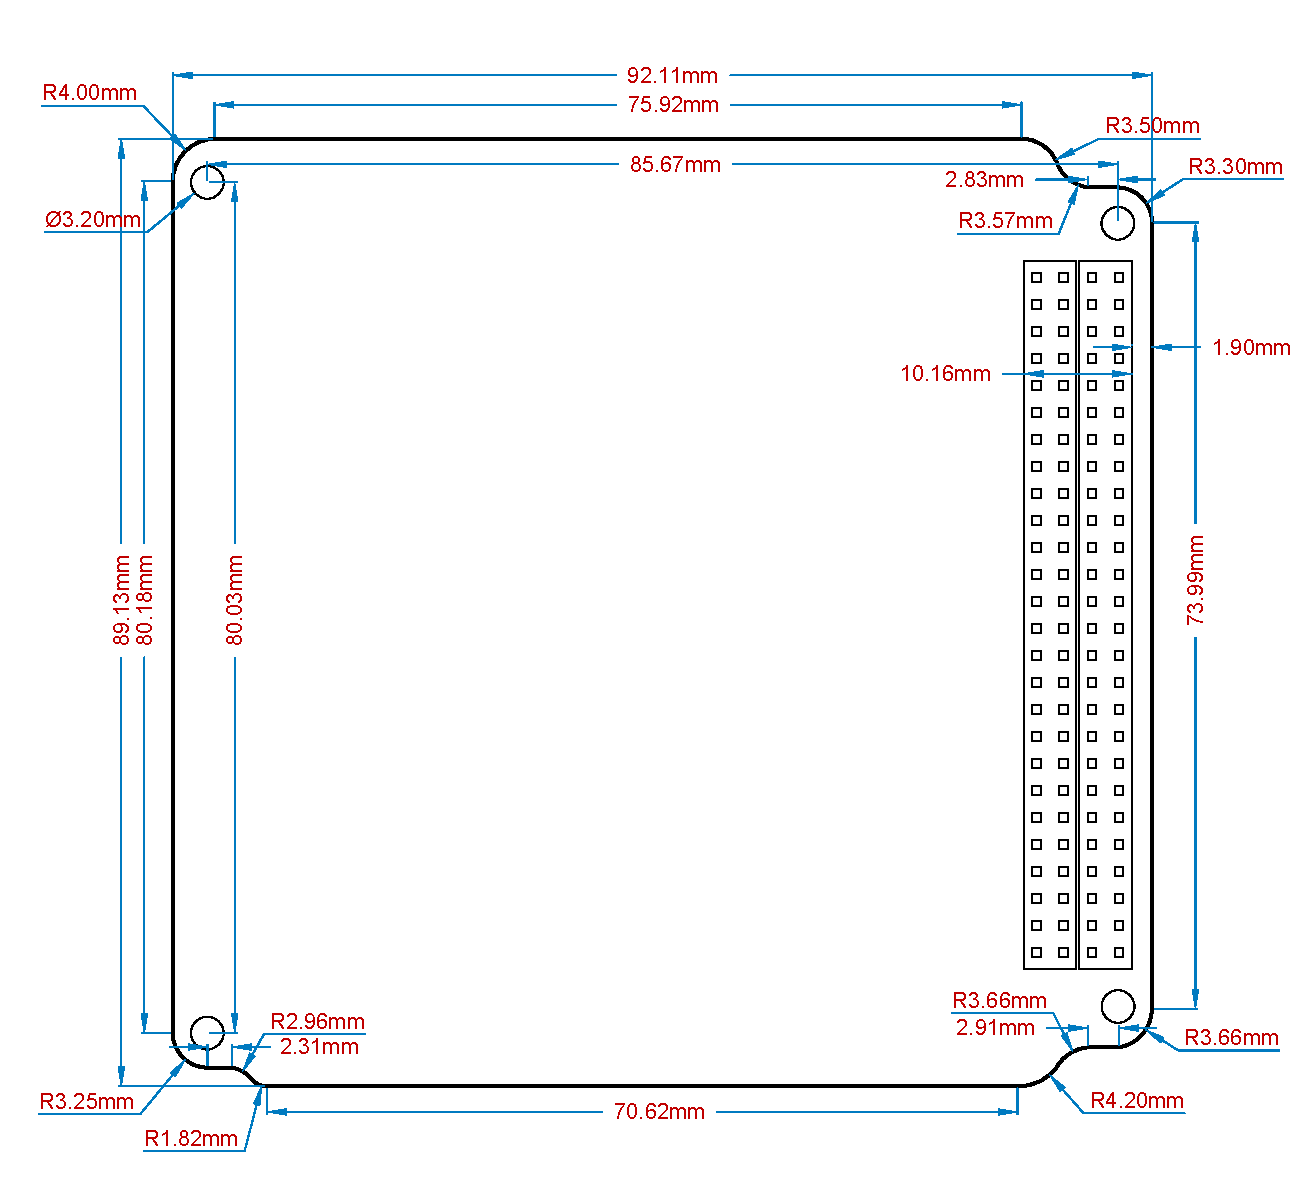
\includegraphics[width=0.75\textwidth]{figures/pc104-form-factor.pdf}
        \caption{PC-104 Form Factor.}
        \label{fig:pc104-form-factor}
    \end{center}
\end{figure}

\section{ \textcolor{red}{TODO} Telecommunication}

This section describes the configuration and behavior of the telecommunication subsystems of the satellite. There are three types of links available in the CubeSat: beacon, downlink, and uplink. The beacon link is a periodic transmission of packets with basic telemetry data of the satellite (containing data from the EPS or TTC subsystems). The downlink is the link used to receive all data from the satellite, including the results of all experiments, telemetry data, and telecommands feedback. Moreover, the uplink sends telecommands from a ground station to the satellite.

The payload of all packets follows the same structure, with an ID number, the source address (callsign), and the packet's content (variable according to each type of packet). Following the NGHam protocol characteristics, the maximum packet length, including the ID and the source address, is 220 bytes. The \autoref{fig:fsat-pkt-structure} illustrates this packet structure.

\begin{figure}[!htb]
    \begin{center}
        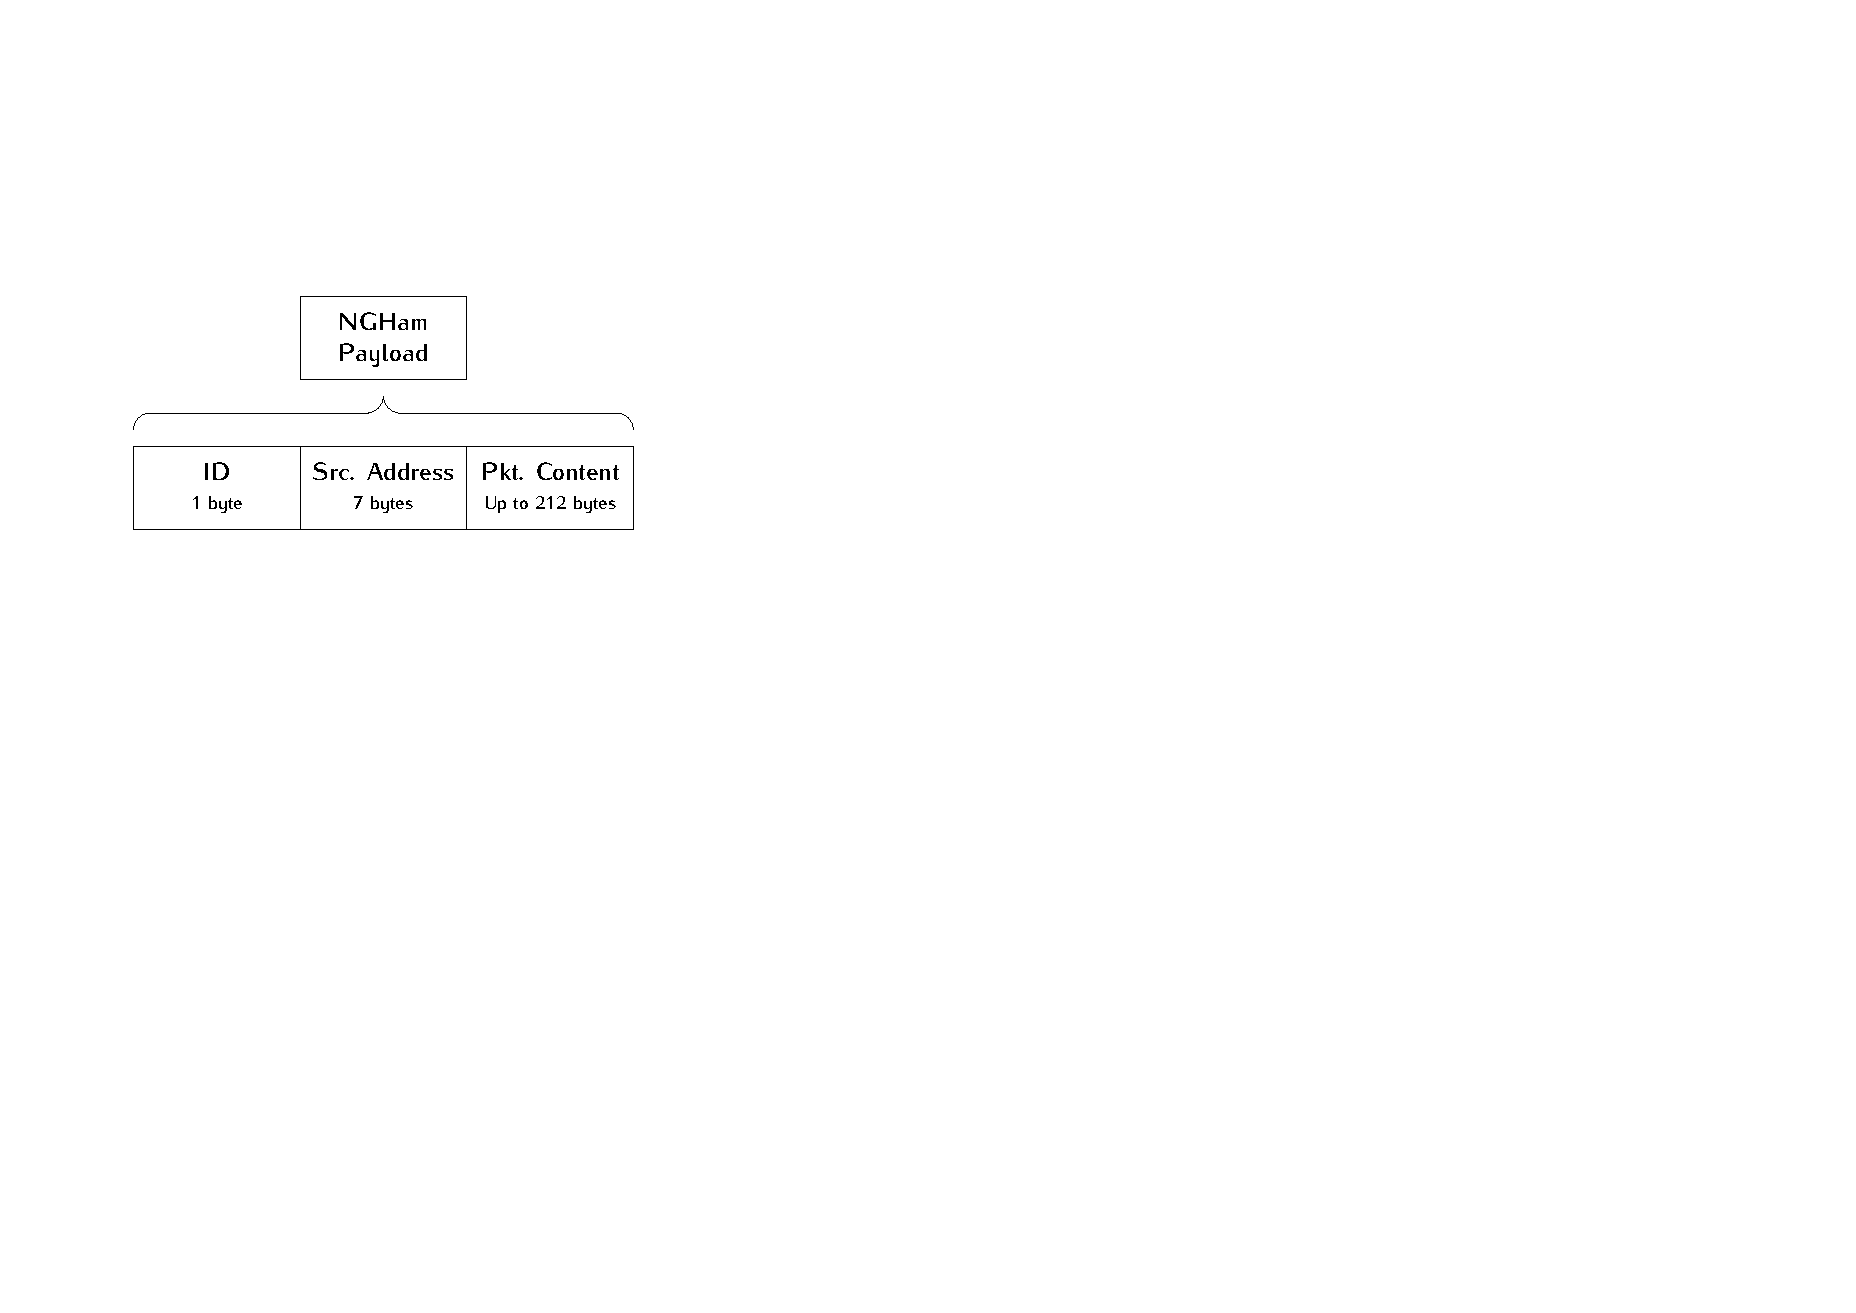
\includegraphics[width=0.5\textwidth]{figures/floripasat-packet-structure.pdf}
        \caption{Payload structure of the Radio Occultation packets.}
        \label{fig:fsat-pkt-structure}
    \end{center}
\end{figure}

The \autoref{tab:packets-struct} summarizes all types of packets transmitted or received by satellite, with the ID number, structure and length, and access type of each packet.

\begin{landscape}
    \begin{table}[ht]
        \centering
        \begin{tabular}{L{1.8cm}lcllcc}
            \toprule[1.5pt]
            \multirow{2}{*}{\textbf{Link}} & \multirow{2}{*}{\textbf{Packet Name}} & \multicolumn{4}{c}{\textbf{Payload}} & \multirow{2}{*}{\textbf{Access}} \\
            \cmidrule{3-6}
                                     &                     & \textbf{ID} & \textbf{Source Callsign} & \textbf{Data (up to 212 bytes)} & \textbf{Size (bytes)} & \\
            \midrule
            Downlink                 & EPS data            & 00h & \multirow{3}{*}{`` '' + ``PY0EFS''} & EPS data                                          & 46        & Public \\
            (VHF)                    & Message broadcast   & 01h &                                     & Requester + dst. callsign + message               & 22 to 60  & Public \\
                                     & Ping answer         & 02h &                                     & Requester callsign                                & 15        & Public \\
            \midrule
                                     & General telemetry   & 10h & \multirow{6}{*}{`` '' + ``PY0EFS''} & OBDH/EPS data                                     & 78        & Public \\
                                     & Data request answer & 11h &                                     & Requester callsign + data ID + ts. + data         & 20 to 220 & Public \\
            Downlink                 & Payload data        & 12h &                                     & Payload ID + payload data                         & 9 to 220  & Public \\
            (UHF)                    & TC feedback         & 13h &                                     & Req. callsign + TC packet ID + timestamp          & 20        & Public \\
                                     & Parameter value     & 14h &                                     & Req. callsign + Sub. ID + Param. ID + Param. Val. & 21        & Public \\
                                     & Packet broadcast    & 15h &                                     & Data of ``Transmit packet'' TC                    & 8 to 60   & Public \\
            \midrule
            \multirow{16}{*}{Uplink} & Ping request        & 40h & \multirow{15}{*}{Any Callsign}      & None                                              & 8         & Public \\
                                     & Data request        & 41h &                                     & Data ID + Start ts. + End ts. + Hash              & 37        & Private \\
                                     & Broadcast Message   & 42h &                                     & Dst. callsign + message                           & 15 to 53  & Public \\
                                     & Enter hibernation   & 43h &                                     & Hibernation in hours + Hash                       & 30        & Private \\
                                     & Leave hibernation   & 44h &                                     & Hash                                              & 28        & Private \\
                                     & Activate module     & 45h &                                     & Module ID + Hash                                  & 29        & Private \\
                                     & Deactivate module   & 46h &                                     & Module ID + Hash                                  & 29        & Private \\
                                     & Activate payload    & 47h &                                     & Payload ID + Hash                                 & 29        & Private \\
                                     & Deactivate payload  & 48h &                                     & Payload ID + Hash                                 & 29        & Private \\
                                     & Erase memory        & 49h &                                     & Hash                                              & 28        & Private \\
                                     & Force reset         & 4Ah &                                     & Hash                                              & 28        & Private \\
                                     & Get payload data    & 4Bh &                                     & Payload ID + Args. + Hash                         & 41        & Private \\
                                     & Set parameter       & 4Ch &                                     & Subsystem ID + Param. ID + Param. value + Hash    & 34        & Private \\
                                     & Get parameter       & 4Dh &                                     & Subsystem ID + Parameter ID + Hash                & 30        & Private \\
                                     & Transmit packet     & 4Eh &                                     & Any sequence of bytes + Hash                      & 8 to 60   & Private \\
                                     & Update TLE          & 4Fh &                                     & Line + TLE line + Hash                            & 98        & Private \\
            \bottomrule[1.5pt]
        \end{tabular}
        \caption{Telecommunication packets and their content.}
        \label{tab:packets-struct}
    \end{table}
\end{landscape}

The ID of the subsystems, modules, and payloads are available in \autoref{tab:system-ids}.

\begin{table}[ht]
    \centering
    \begin{tabular}{lcl}
        \toprule[1.5pt]
        \textbf{Type} & \textbf{ID Number} & \textbf{Description} \\
        \midrule
        \multirow{4}{*}{Subsystem} & 0 & OBDH \\
                                   & 1 & TTC 1 \\
                                   & 2 & TTC 2 \\
                                   & 3 & EPS \\
        \midrule
        \multirow{3}{*}{Module}    & 1 & Battery heater \\
                                   & 2 & Beacon \\
                                   & 3 & Periodic telemetry \\
        \midrule
        \multirow{4}{*}{Payload}   & 1 & EDC 1 \\
                                   & 2 & EDC 2 \\
                                   & 3 & Radiation instrument \\
        \bottomrule[1.5pt]
    \end{tabular}
    \caption{IDs of the satellite.}
    \label{tab:system-ids}
\end{table}

\subsection{ \textcolor{red}{TODO} Authentication}

All the telecommands classified as private use an HMAC\nomenclature{\textbf{HMAC}}{\textit{Hash-based Message Authenticaion Code.}} authentication scheme. Every type of private telecommand has a unique 16-digit ASCII character key that with the telecommand sequence (or message) generates an 160-bits (20-bytes) hash sequence to be transmitted together with the packet payload. The used hash algorithm is the SHA-1\nomenclature{\textbf{SHA-1}}{\textit{Secure Hash Algorithm 1.}}. The \autoref{fig:hmac-diagram} illustrates this authentication method.

\begin{figure}[!htb]
    \begin{center}
        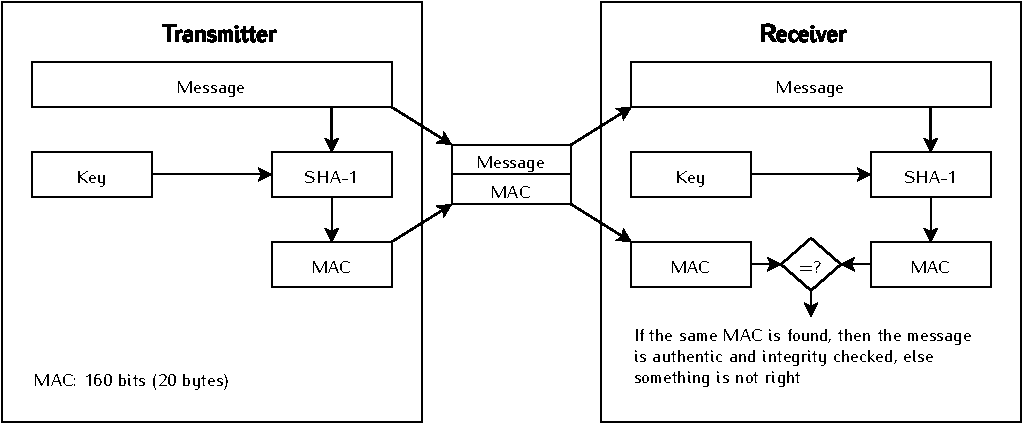
\includegraphics[width=\textwidth]{figures/hmac-diagram.pdf}
        \caption{Diagram of the used HMAC scheme.}
        \label{fig:hmac-diagram}
    \end{center}
\end{figure}

\subsection{ \textcolor{red}{TODO} Operation Licenses}

%\textcolor{red}{COMMENT: tiramos essa parte?}

Regarding the non-amateur radios frequencies, Resolution 685, of October 9, 2017 from ANATEL establishes that:

Art. 9. Assign to the Private Limited Service (SLP), for use by systems for capturing and transmitting scientific data related to space operation, on a secondary basis, the following sub-ranges (related to this project):

\begin{itemize}
\item 400.15 MHz to 401 MHz;
\item 449.75 MHz to 450.25 MHz.
\end{itemize}

Art. 17. The allocation of all radio frequency bands dealt with in this Resolution follows the restrictions imposed by the respective allocation.

Single paragraph. Those interested in the use of the radio frequency bands object of this Resolution must provide in their projects, until specific regulations are issued on the conditions of use of these bands, criteria for harmonious coexistence with the existing systems in these bands, maintaining specific coordination, when necessary, of such so that incoming systems do not cause harmful interference to existing systems.

Thus, a process must be carried out for radio 1 (146 MHz) in the amateur radio band, and another process for the radios with 401 MHz and 450 MHz. Since the last two radios must be a secondary service SLP where a preliminary study is necessary on the harmonic coexistence with the existing systems in these bands.

    %
% subsystems.tex
%
% Copyright (C) 2021 by SpaceLab.
%
% Radio Occultation Documentation
%
% This work is licensed under the Creative Commons Attribution-ShareAlike 4.0
% International License. To view a copy of this license,
% visit http://creativecommons.org/licenses/by-sa/4.0/.
%

%
% \brief Subsystems chapter.
%
% \author Gabriel Mariano Marcelino <gabriel.mm8@gmail.com>
%
% \institution Universidade Federal de Santa Catarina (UFSC)
%
% \version 0.2.0
%
% \date 2020/06/06
%

\chapter{ \textcolor{red}{TODO} Subsystems} \label{ch:subsystems}

%, which can be seen in the exploded view of the satellite, available in \autoref{fig:exploded-view}.

%\begin{figure}[!htb]
%    \begin{center}
%        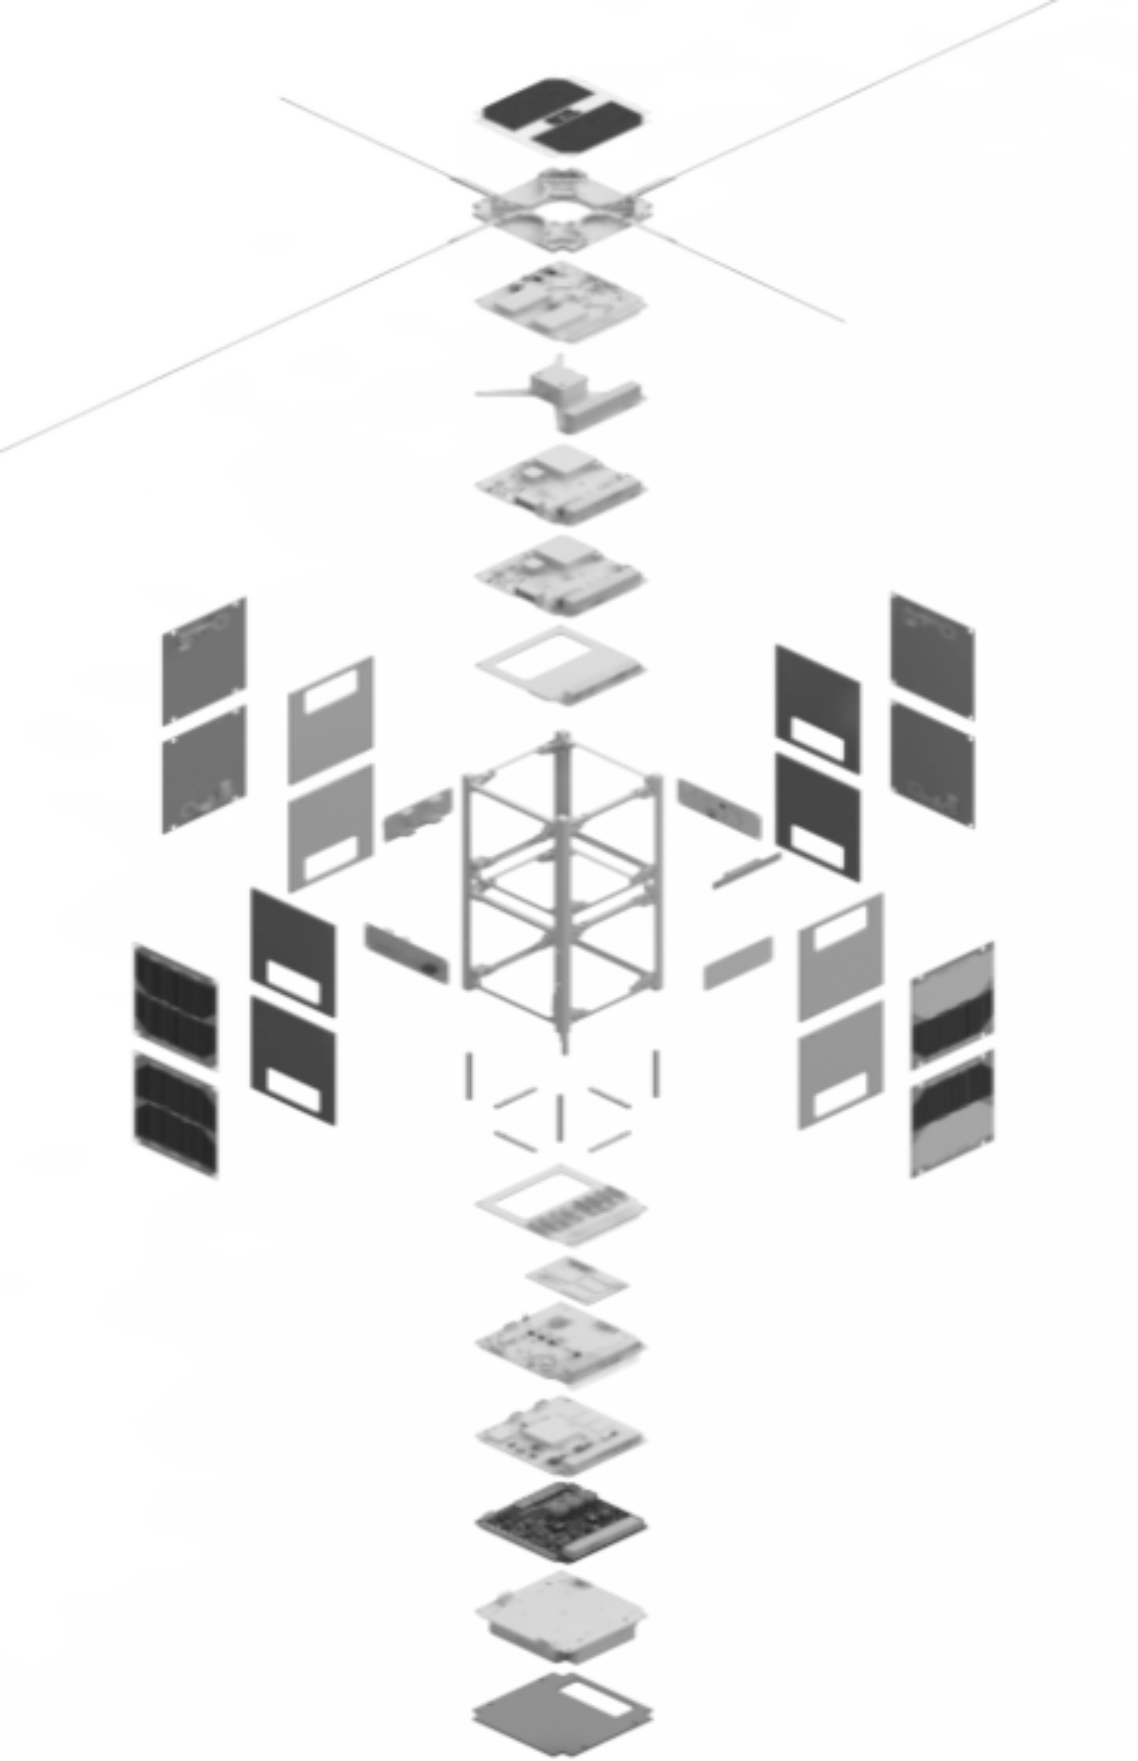
\includegraphics[width=0.35\textwidth]{figures/subsystems/floripasat.png}
%        \caption{Exploded view of the Radio Occultation satellite.}
%        \label{fig:exploded-view}
%    \end{center}
%\end{figure}

This chapter describes all subsystems of the space segment of the mission. Most subsystems presented here have their own technical documentation with a more profound description. When available, there is a reference to the respective document. This chapter is intended to show an overview of each subsystem in a macro context of the mission.

\section{ \textcolor{red}{TODO} Radio Occultation Instrument}


\section{ \textcolor{red}{TODO} Radio Occultation Instrument Antenna}


\section{ \textcolor{red}{TODO} Attitude Control System}

The Attitude Control System (ACS\nomenclature{\textbf{ACS}}{\textit{Attitude Control System}.}) is a passive attitude control system, which depends on the Earth's magnetic field to rotate and stabilize the satellite \cite{santoni2009,gerhardt2010}. The system is composed of one permanent magnet to create a force to align the magnet with the Earth's magnetic field and four hysteresis bars to dampen the cube oscillations and achieve stabilization.

When equilibrium is achieved, the permanent magnet aligns with the Earth's field lines. The hysteresis bars convert oscillation and rotation energy into heat, maintaining the alignment through the magnetic moment. The components are placed in positions to minimize the magnet's interaction with the hysteresis bars, which limits the magnetic moment of the magnet \cite{francois2010}. \autoref{fig:adcs} shows the mounting of the hysteresis bars (green) and the permanent magnet (red) on the mechanical structure. The whole passive ACS was implemented according to \cite{francois2010}.

\begin{figure}[!ht]
    \begin{center}
        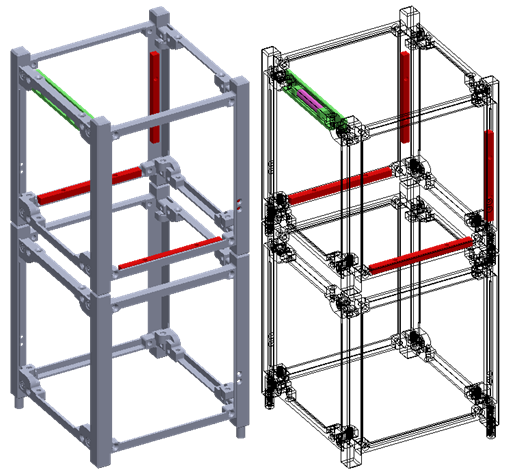
\includegraphics[width=0.7\textwidth]{figures/subsystems/adcs}
        \caption{ACS subsytem. Rare earth magnet (pink) and hysteresis bars (red) installed in the structure.}
        \label{fig:adcs}
    \end{center}
\end{figure}

As a passive magnetic attitude control system is used, it is possible to stabilize only one axis. So, the CubeSat will still slowly (due to hysteresis bars) rotate around this axis, even after stabilized. A N45 neodymium magnet and 4 hysteresis bars of Permanorm 5000 H2 are used (courtesy of Vacuumschmelze GmbH \& Co. KG). The hysteresis bar's material is shaped to maximize stabilization, which is the most critical part of attitude control.

Many conditions impact the detumbling time, which is the time required for the satellite to stabilize. Magnetic passive attitude stabilization systems such as the one developed for this mission achieve the equilibrium state within a few weeks of operation \cite{santoni2009}.

The Radio Occultation satellite does not feature an orbit control subsystem.


\section{ \textcolor{yellow}{Doing} S-Band Antenna}

\section{ \textcolor{yellow}{Doing} GNSS Antenna}

\section{ \textcolor{yellow}{Doing} Antenna Module}

The SpaceLab Deployable Antenna Module is the first flight-capable version developed at SpaceLab. It is a four monopole antenna built with tape strings and compliant with the CubeSat standard. The deployment method is the burning wire, which can be controlled digitally through a CAN interface. To allow redundancy, two independent deployment controllers can be activated separately. Also, the construction of this module allows the installation of a solar panel at the top side.

A picture of the antenna module (with all antennas released) can be seen in \autoref{fig:sl-antenna}. The chosen antenna configuration for this mission its V-dipole. To learn more about the different configurations, see \cite{ant-rad}.

\begin{figure}[!ht]
    \begin{center}
        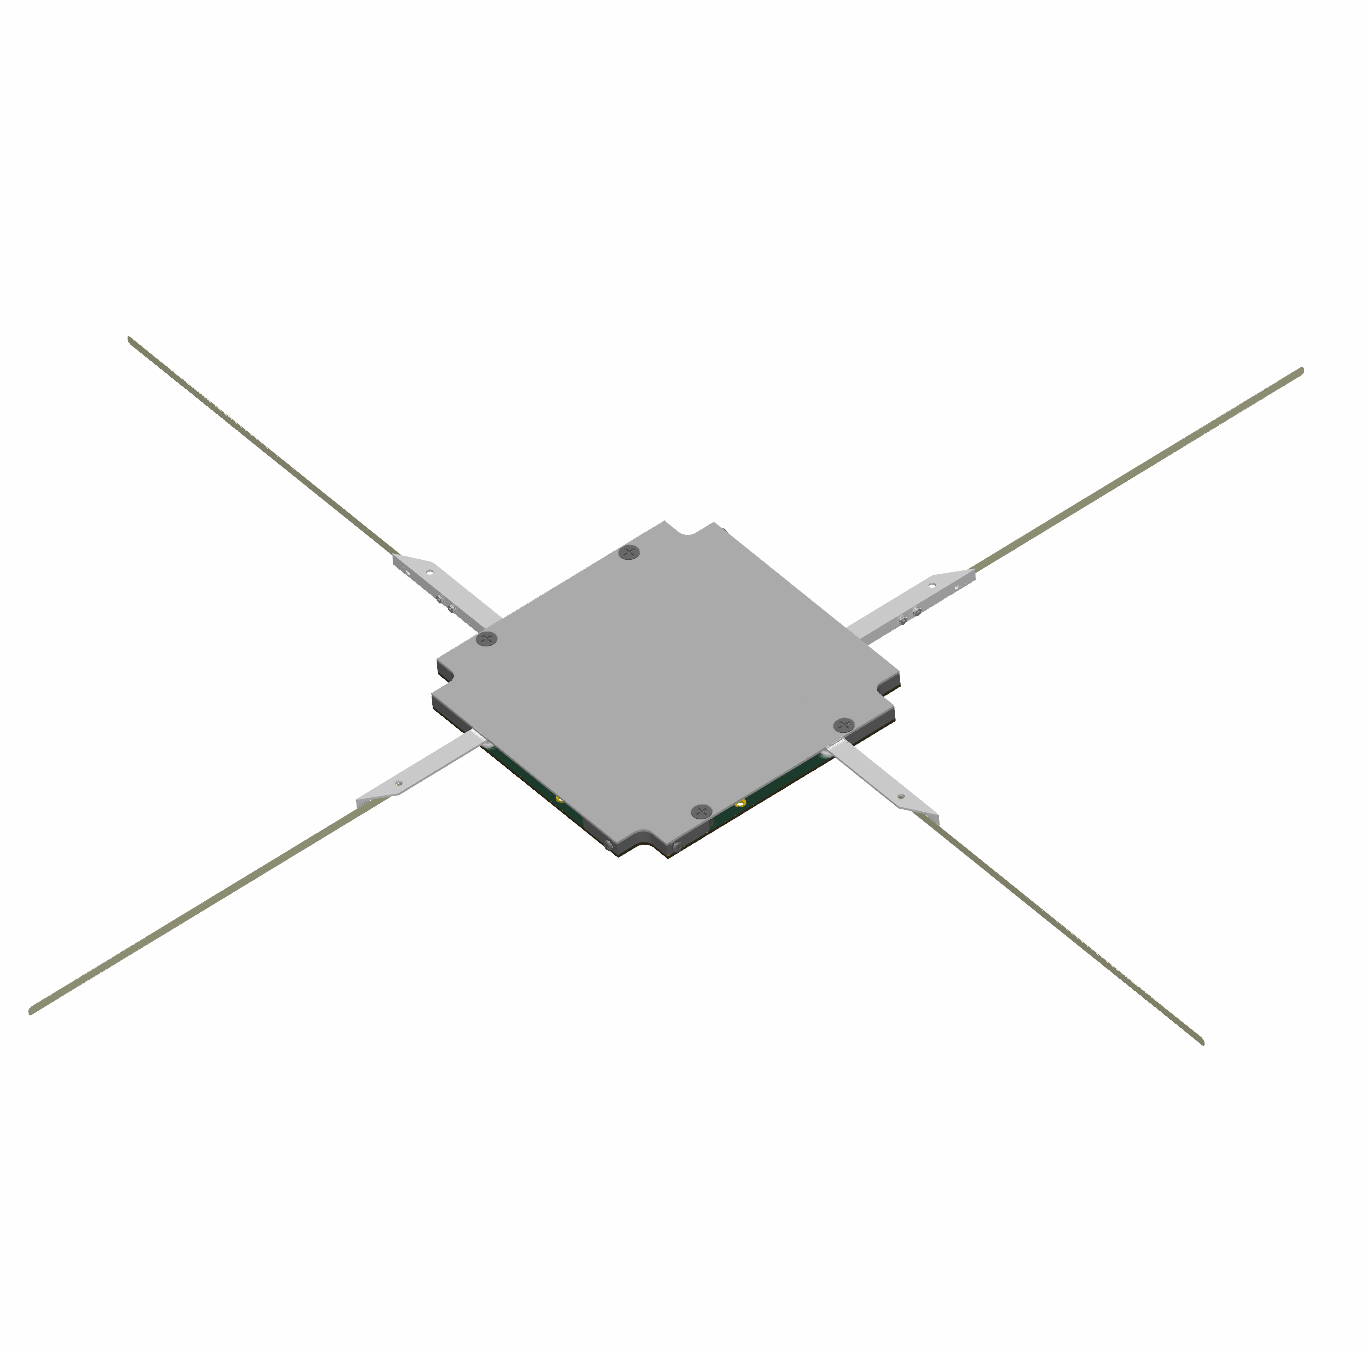
\includegraphics[width=0.8\textwidth]{figures/subsystems/sl-antenna.png}
        \caption{SpaceLab Deployable Antenna Module}
        \label{fig:sl-antenna}
    \end{center}
\end{figure}


\begin{itemize}
    \item Configuration: 2 V-dipoles 
        \begin{itemize}
            \item Antenna 1: UHF - \textcolor{red}{TBD} MHz (downlink)
            \item Antenna 2: UHF - \textcolor{red}{TBD} MHz (uplink)
        \end{itemize}
    \item Tuning structure size: 6U
    \item Mounting position: Top and Bottom
    \item Supply voltage: 3.3 V
    \item CAN 
        \begin{itemize}
            \item Primary CAN address: \textcolor{red}{TBD} (\textcolor{red}{TBD}-bit address)
            \item Redundant CAN address: \textcolor{red}{TBD} (\textcolor{red}{TBD}-bit address)
        \end{itemize}
\end{itemize}

\begin{figure}[!ht]
    \begin{center}
        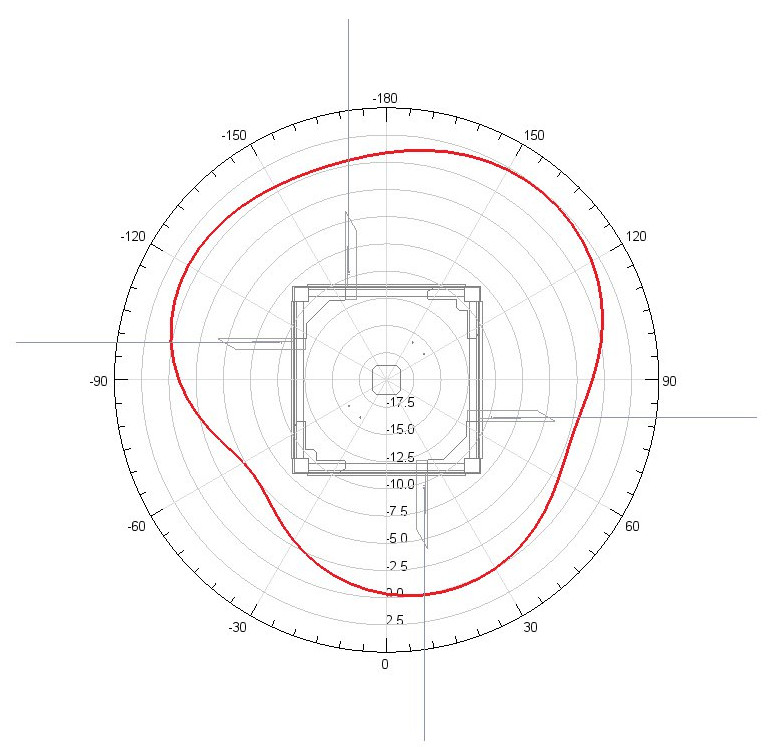
\includegraphics[width=0.7\textwidth]{figures/subsystems/sat_2drad_dipv_z.jpg}
        \caption{ Gain diagram of the antenna in V-dipole configuration in the z plane \cite{ant-rad}.}
        \label{fig:ant-rad}
    \end{center}
\end{figure}

The radiation diagram of the antenna in the v-dipole configuration can be seen in \autoref{fig:ant-rad}.

\section{ \textcolor{red}{TODO} On-Board Data Handling}

The OBDH\nomenclature{\textbf{OBDH}}{\textit{On-Board Data Handling}.} 2.0 is an On-Board Computer (OBC) module designed for nanosatellites. The module is responsible for synchronizing actions and the data flow between other modules (i.e., power module, communication module, payloads) and the Earth segment. It packs the generated data into data frames and transmits back to Earth through a communication module or stores it on non-volatile memory for later retrieval. Commands sent from Earth segment to the CubeSat are received by radio transceivers in the communication module and redirected to the OBDH, which takes the appropriate action or forward the commands to the target module.

The module is a direct upgrade from the OBDH of Radio Occultation \cite{floripasat}, which grants a flight heritage rating. The improvements focus on providing a cleaner and more generic implementation than the previous version, more reliability in software and hardware implementations, and adaptations for the new mission requirements. The module board can be seen in \autoref{fig:obdh2}.

\begin{figure}[!ht]
    \begin{center}
        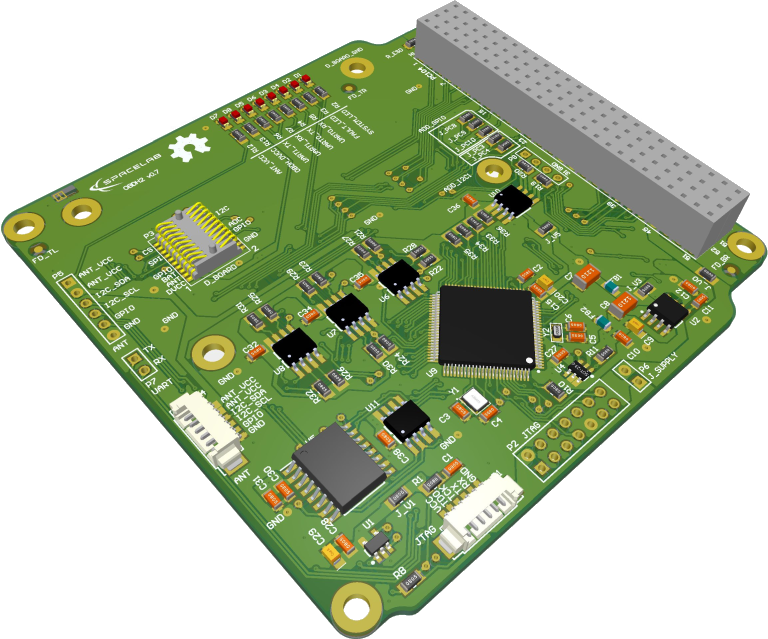
\includegraphics[width=0.7\textwidth]{figures/subsystems/obdh2-pcb-3d}
        \caption{OBDH module.}
        \label{fig:obdh2}
    \end{center}
\end{figure}

More information about this module can be found in \cite{obdh2}.

\section{ \textcolor{red}{TODO} Telemetry, Tracking and Command Module}

The TTC\nomenclature{\textbf{TTC}}{\textit{Telemetry, Tracking and Command Module}.} (or TT\&C) is responsible for making the communication between the Earth (a ground station) and the satellite and is divided into two sub-modules: Beacon and downlink/uplink. The beacon is an independent sub-module that transmits a periodic signal containing satellite identification data (ID) and some basic telemetry data. The downlink/uplink sub-module is the primary communication device. It has a bidirectional data link to receive telecommands from the Earth and transmit all available data back to Earth. The module board can be seen in \autoref{fig:ttc}.

\begin{figure}[!ht]
    \begin{center}
        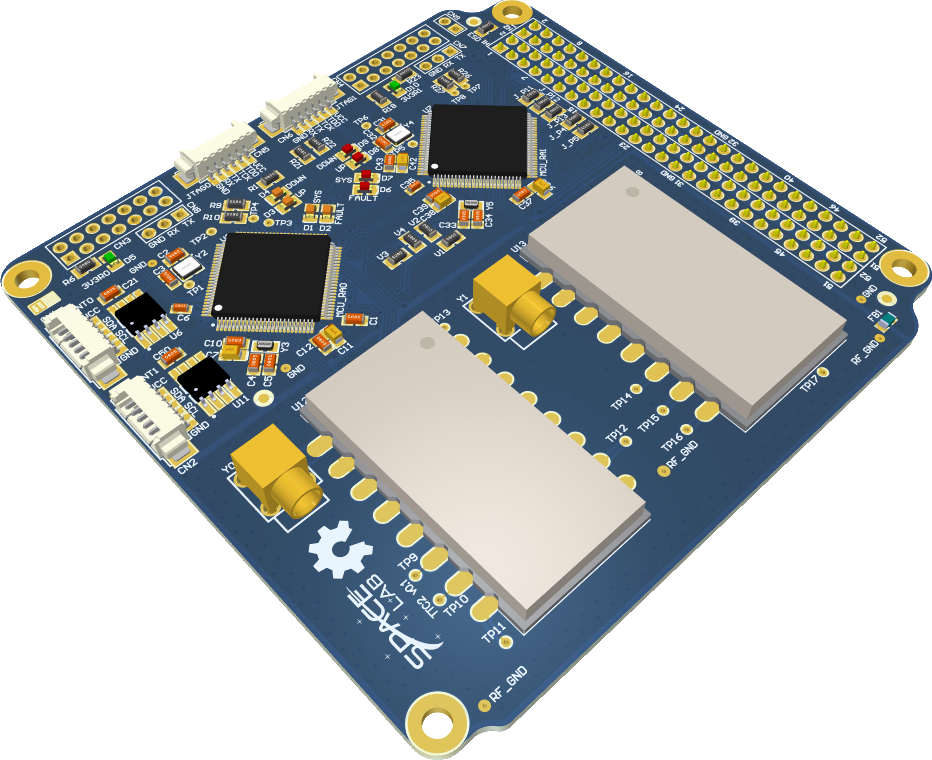
\includegraphics[width=0.7\textwidth]{figures/subsystems/ttc2_pcb_3d}
        \caption{TTC module.}
        \label{fig:ttc}
    \end{center}
\end{figure}

More information about this module can be found in \cite{ttc}.


\section{ \textcolor{red}{TODO} Electrical Power System}

The EPS\nomenclature{\textbf{EPS}}{\textit{Electrical Power System}.} is the module designed to harvest, store and distribute energy for the satellite. The energy harvesting system is based on solar energy conversion through the solar panels attached to the CubeSat structure. The EPS is designed to operate the solar panels at their maximum power point (MPPT\nomenclature{\textbf{MPPT}}{\textit{Maximum Power Point Tracking}.}). The board also measures the solar panels current, voltage and temperature of the batteries. The harvested solar energy is stored in a battery module connected to the EPS. Several integrated buck DC-DC converters do the energy distribution. The full Radio Ocultation EPS system is composed of the solar panels, two EPS PCBs\nomenclature{\textbf{PCB}}{\textit{Printed Circuit Board.}} and two battery modules. A general view of the EPS board can be seen in \autoref{fig:eps2}.

\begin{figure}[!ht]
    \begin{center}
        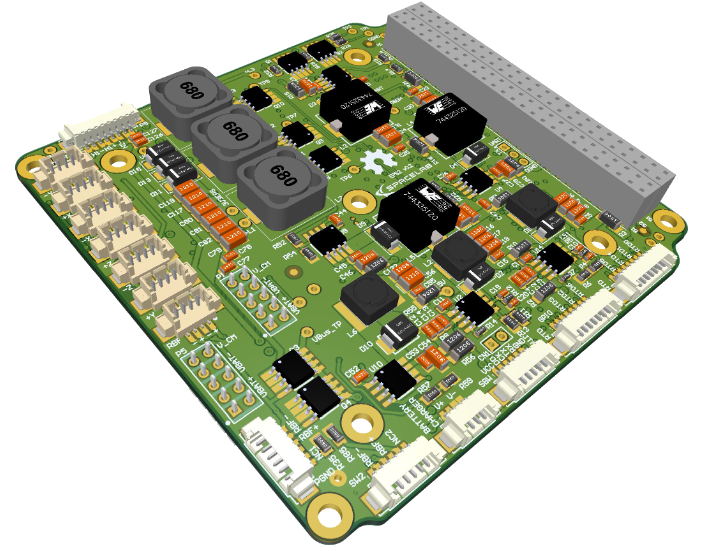
\includegraphics[width=0.7\textwidth]{figures/subsystems/eps2-pcb-3d}
        \caption{EPS module.}
        \label{fig:eps2}
    \end{center}
\end{figure}

This EPS module is the same board used in GOLDS \textcolor{red}{[FloripaSat-2]} which grants a flight heritage rating. % \cite{floripasat}, . The improvements focus on providing a cleaner and more generic implementation compared to the previous version, more reliability in software, and adaptations for the new mission requirements.

More information about this module can be found in \cite{eps2}.

\subsection{ \textcolor{red}{TODO} Battery Module} \label{ssec:battery-module}

The used battery module is the ``\textit{Battery Module 4C}'', which is a separate battery module from the EPS board and composed by four lithium-ion 18650 cells. Besides the cells, the board has connectors for interfacing signals and power lines with the EPS module, 2 power resistors to operate as heaters to maintain the cell's temperature during eclipse periods, and 4 temperature sensors. The batteries used are the ICR18650-30B lithium-ion cells from Samsung \cite{icr18650-30b}, which are connected in series and parallel (two sets of two parallel cells in series) to supply the required voltage and current. Each cell is fixed with 18650 metal holders, and between the pairs, the power resistor is attached with a thermal element in the middle. A mechanical mount is placed over the batteries and screwed to the board, providing better stress resistance. Also, PC-104 through-hole pads are present on the board for a connector that could be used for mechanical integration with the EPS, or, with future improvements, an interface for power, data or control signals. The board is a direct improvement from the first battery board used in the Radio Occultation mission \cite{floripasat}.

\begin{figure}[!ht]
    \begin{center}
        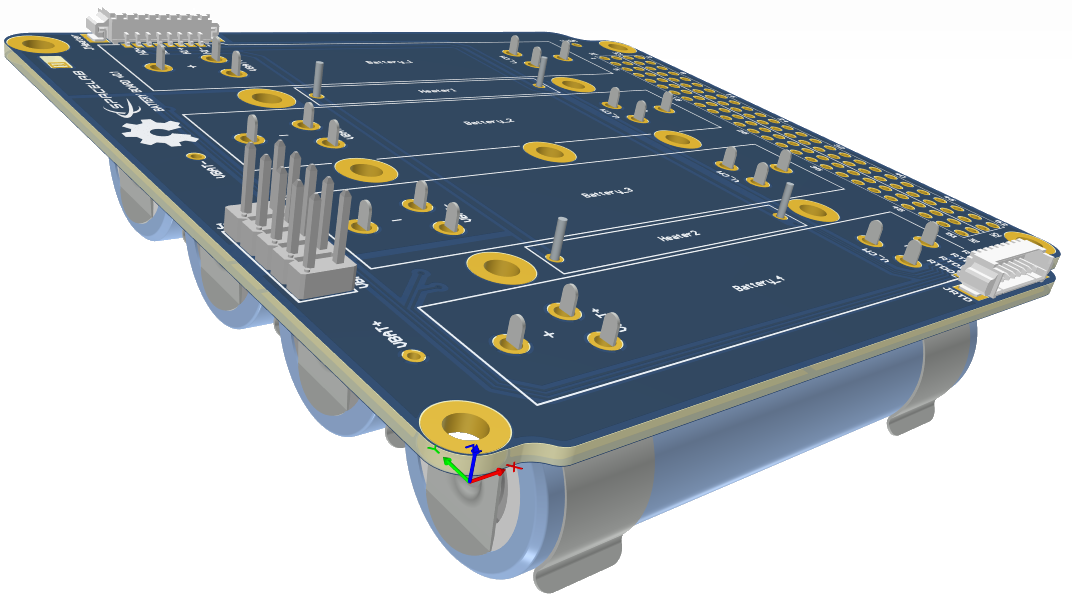
\includegraphics[width=0.7\textwidth]{figures/subsystems/bat2-pcb-3d}
        \caption{Battery module board.}
        \label{fig:battery-module-board}
    \end{center}
\end{figure}

More information about the battery module can be found in \cite{bat4c}.

\subsection{ \textcolor{red}{TODO} Solar Panels}

The solar panels are a set of 17 home-made panels, designed by SpaceLab members. The panels feature protection diodes and a high-efficiency sollar cells, witch are the Triple Junction GaAs SC-3GA-3 \textcolor{red}{[SC-3GA-3]} with dimensions 8.15 $\times$ 4.15 cm (area 30.15 cm$^{2}$). This cell is qualified for space use by ESA with an efficiency of 30 \% (AM0, BOL). The panels do not include magnetometers, sensors, and other devices. 
%The solar panels are a set of 5 custom-made panels manufactured by ORBITAL, a Brazilian company, and a single panel from ISISpace. The panels feature protection diodes and high-efficiency solar cells, which are the CESI's CTJ-30 \cite{ctj30} with dimensions 6.9 $\times$ 3.9 cm (area 26.5 cm$^{2}$). This cell is qualified for space use by ESA with an efficiency of 29.5 \% (AM0, BOL). The panels do not include magnetometers, sensors, and other devices. The top solar panel is a model from ISISpace to ensure mechanical compatibility with the antenna module (also from ISISpace). These two types of solar panels can be seen in Figures \ref{fig:solar-panel-orbital} and \ref{fig:top-solar-panel}.

\begin{figure}[!ht]
    \begin{center}
        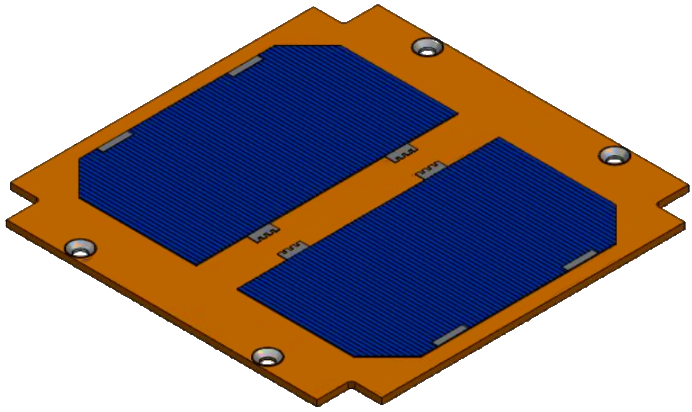
\includegraphics[width=0.7\textwidth]{figures/subsystems/orbital-solar-panel}
        \caption{Conceptual solar panel from ORBITAL.}
        \label{fig:solar-panel-orbital}
    \end{center}
\end{figure}

\begin{figure}[!ht]
    \begin{center}
        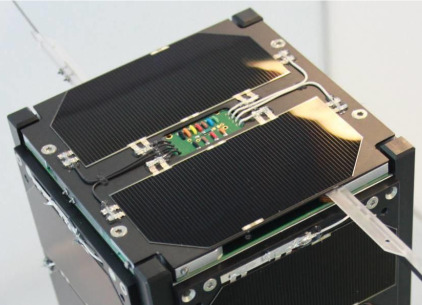
\includegraphics[width=0.6\textwidth]{figures/subsystems/isis-top-solar-panel}
        \caption{Top solar panel from ISISpace.}
        \label{fig:top-solar-panel}
    \end{center}
\end{figure}

\subsection{ \textcolor{red}{TODO} Kill-Switches and RBF}

Two electronic switches have been implemented into the design to allow for the (redundant) deployment detection of the CubeSat when deployed from the POD. This electronic micro switch can be used to prevent the satellite from starting up during launch, as is required for all CubeSat launches and hence acts as a Kill-Switch. The Kill-Switch is the Panasonic AV4 microswitch (AV402461), as seen in \autoref{fig:av402461}.

\begin{figure}[!ht]
    \begin{center}
        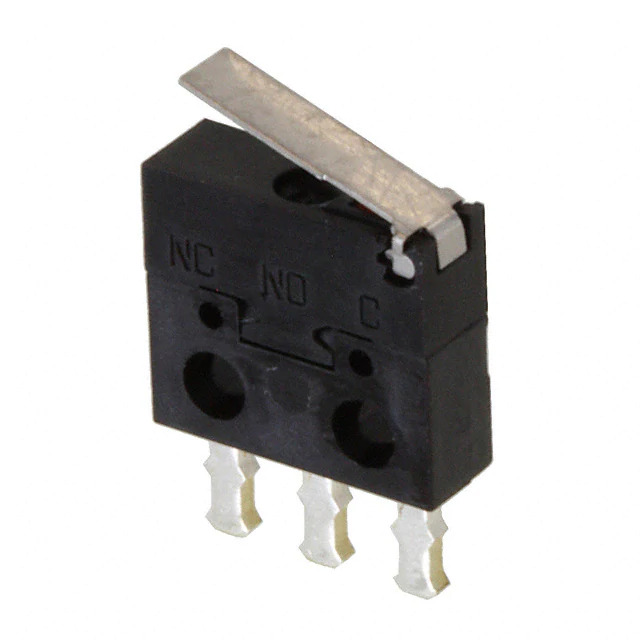
\includegraphics[width=0.25\textwidth]{figures/subsystems/av402461}
        \caption{Panasonic AV402461 Microswitch.}
        \label{fig:av402461}
    \end{center}
\end{figure}

The Kill-Switch mechanism in the mechanical structure has combined the function of providing deployment and detection (\autoref{fig:kill-switch-installed}). The travel of the actual switch of the Kill-Switch itself is so short that the Kill-Switch could ``detect deployment'' of the CubeSat from the launch adapter simply due to launch vibrations. To overcome this issue the Kill-Switch has been rotated so that there is a positive obstruction in front of the switch which needs 8 mm of deployment before deployment can be detected with the Kill-Switch. In \autoref{fig:kill-switch-installed} the Kill-Switch parts are highlighted, and the stowed and deployed configuration is shown.

\begin{figure}[!ht]
    \begin{center}
        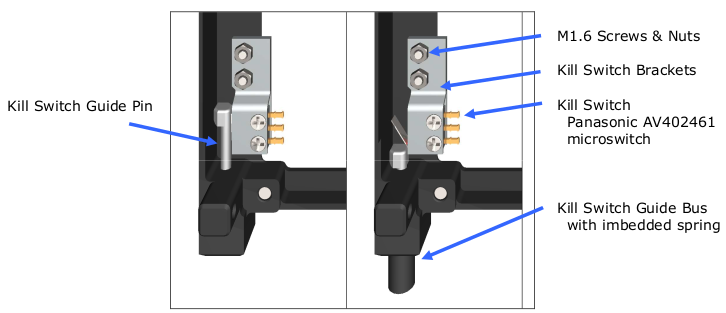
\includegraphics[width=0.85\textwidth]{figures/subsystems/kill-switch-installed}
        \caption{Kill-Switches installed in the mechanical structure.}
        \label{fig:kill-switch-installed}
    \end{center}
\end{figure}

The contact arrangement of the microswitch and the current rating are detailed in \autoref{fig:circuit-kill-switch} and \autoref{tab:kill-switch-specs}.

\begin{figure}[!ht]
    \begin{center}
        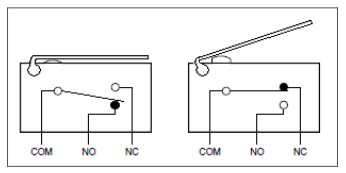
\includegraphics[width=0.4\textwidth]{figures/subsystems/circuit-kill-switch}
        \caption{The contact arrangement of the microswitch.}
        \label{fig:circuit-kill-switch}
    \end{center}
\end{figure}

\begin{table}[!h]
    \centering
    \begin{tabular}{lcccc}
        \toprule[1.5pt]
        \textbf{Characteristic} & \textbf{Minimum} & \textbf{Typical} & \textbf{Maximum} & \textbf{Unit} \\
        \midrule
        Switch Current                      & 2     & 50    & 100   & mA \\
        DC Voltage across switch contacts   & n/a   & n/a   & 30    & V \\
        Contact resistance microswitch      & n/a   & n/a   & 200   & m$\Omega$ \\
        \bottomrule[1.5pt]
    \end{tabular}
    \caption{Kill-Switch current rating and voltage range.}
    \label{tab:kill-switch-specs}
\end{table}


\section{ \textcolor{red}{TODO} Thermal control}

An active control gives the thermal control: two resistors (24 $\Omega$) to protect the batteries against low temperatures and two RTODOs to monitor the temperature. The control is an ON/OFF control.
%    \item Passive thermal control: two heat pipes connecting opposite solar panels, as illustrated in Figure \ref{fig:HP}. The external diameter is 1/4'', the working fluid is water, the condenser and evaporator sections have 30 mm of length, and the adiabatic section has 90 mm.



\section{ \textcolor{red}{TODO} Mechanical Structure}

The USIPED 2-Unit CubeSat structure is developed as a generic, modular satellite structure based on the CubeSat standard. The modular chassis allows up to two 1-Unit stack of PCBs, or other modules, to be mounted inside the chassis, using the PC-104 standard and spacers attached to the structure. In addition, there are 4 slots in the middle section, providing space for the interface boards and the ACS. The solar panels and antennas are externally mounted, providing a complete mechanical solution. A picture of this structure can be seen in \autoref{fig:usiped-structure}.

\begin{figure}[!ht]
    \begin{center}
        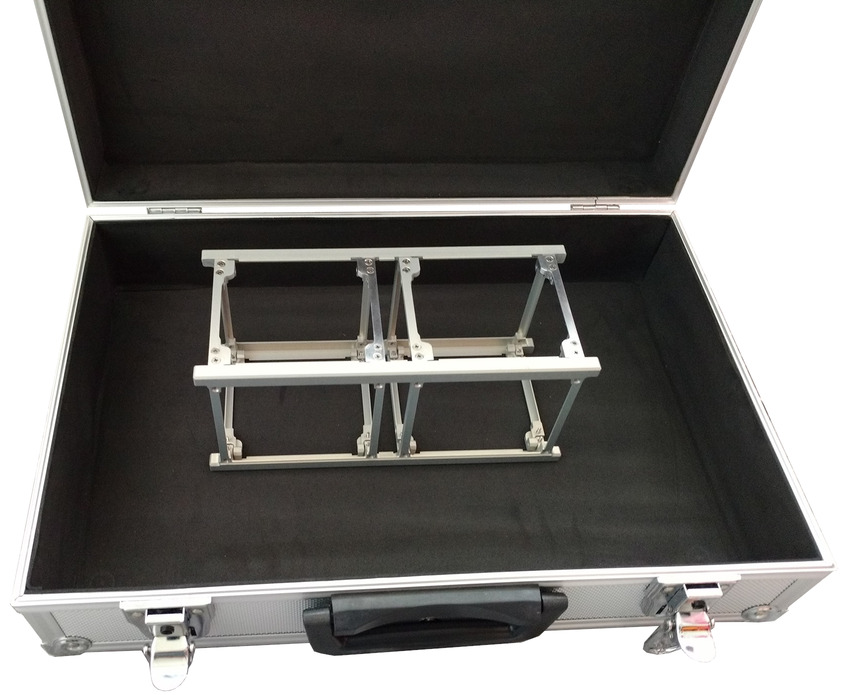
\includegraphics[width=0.7\textwidth]{figures/subsystems/usiped-2u-structure.jpg}
        \caption{2U CubeSat structure from Usiped.}
        \label{fig:usiped-structure}
    \end{center}
\end{figure}

The structure will support the loads and vibration along the entire life cycle of the satellite, which includes every phase prior to the launch, the launch itself, and the operation of the CubeSat in space. In addition, the structure must keep all the parts of the CubeSat fastened at the proper position during the launch and operation, provide a conductive thermal path for heat transfer, and provide access for assembly, integration, and verification.

The material of all its parts is aluminum T6065, except for the bolts and thread. This material presents good mechanical properties for space application, such as weight, strength, fracture and fatigue resistance, thermal expansion, and ease of manufacturing. The surfaces of the CubeSat in contact with the deployer are anodized and grounded for proper and smooth ejection. The main views of the assembled structure is presented in \autoref{fig:structure_views}, as well as its main dimensions.


\begin{figure}[H]
	\begin{center}
		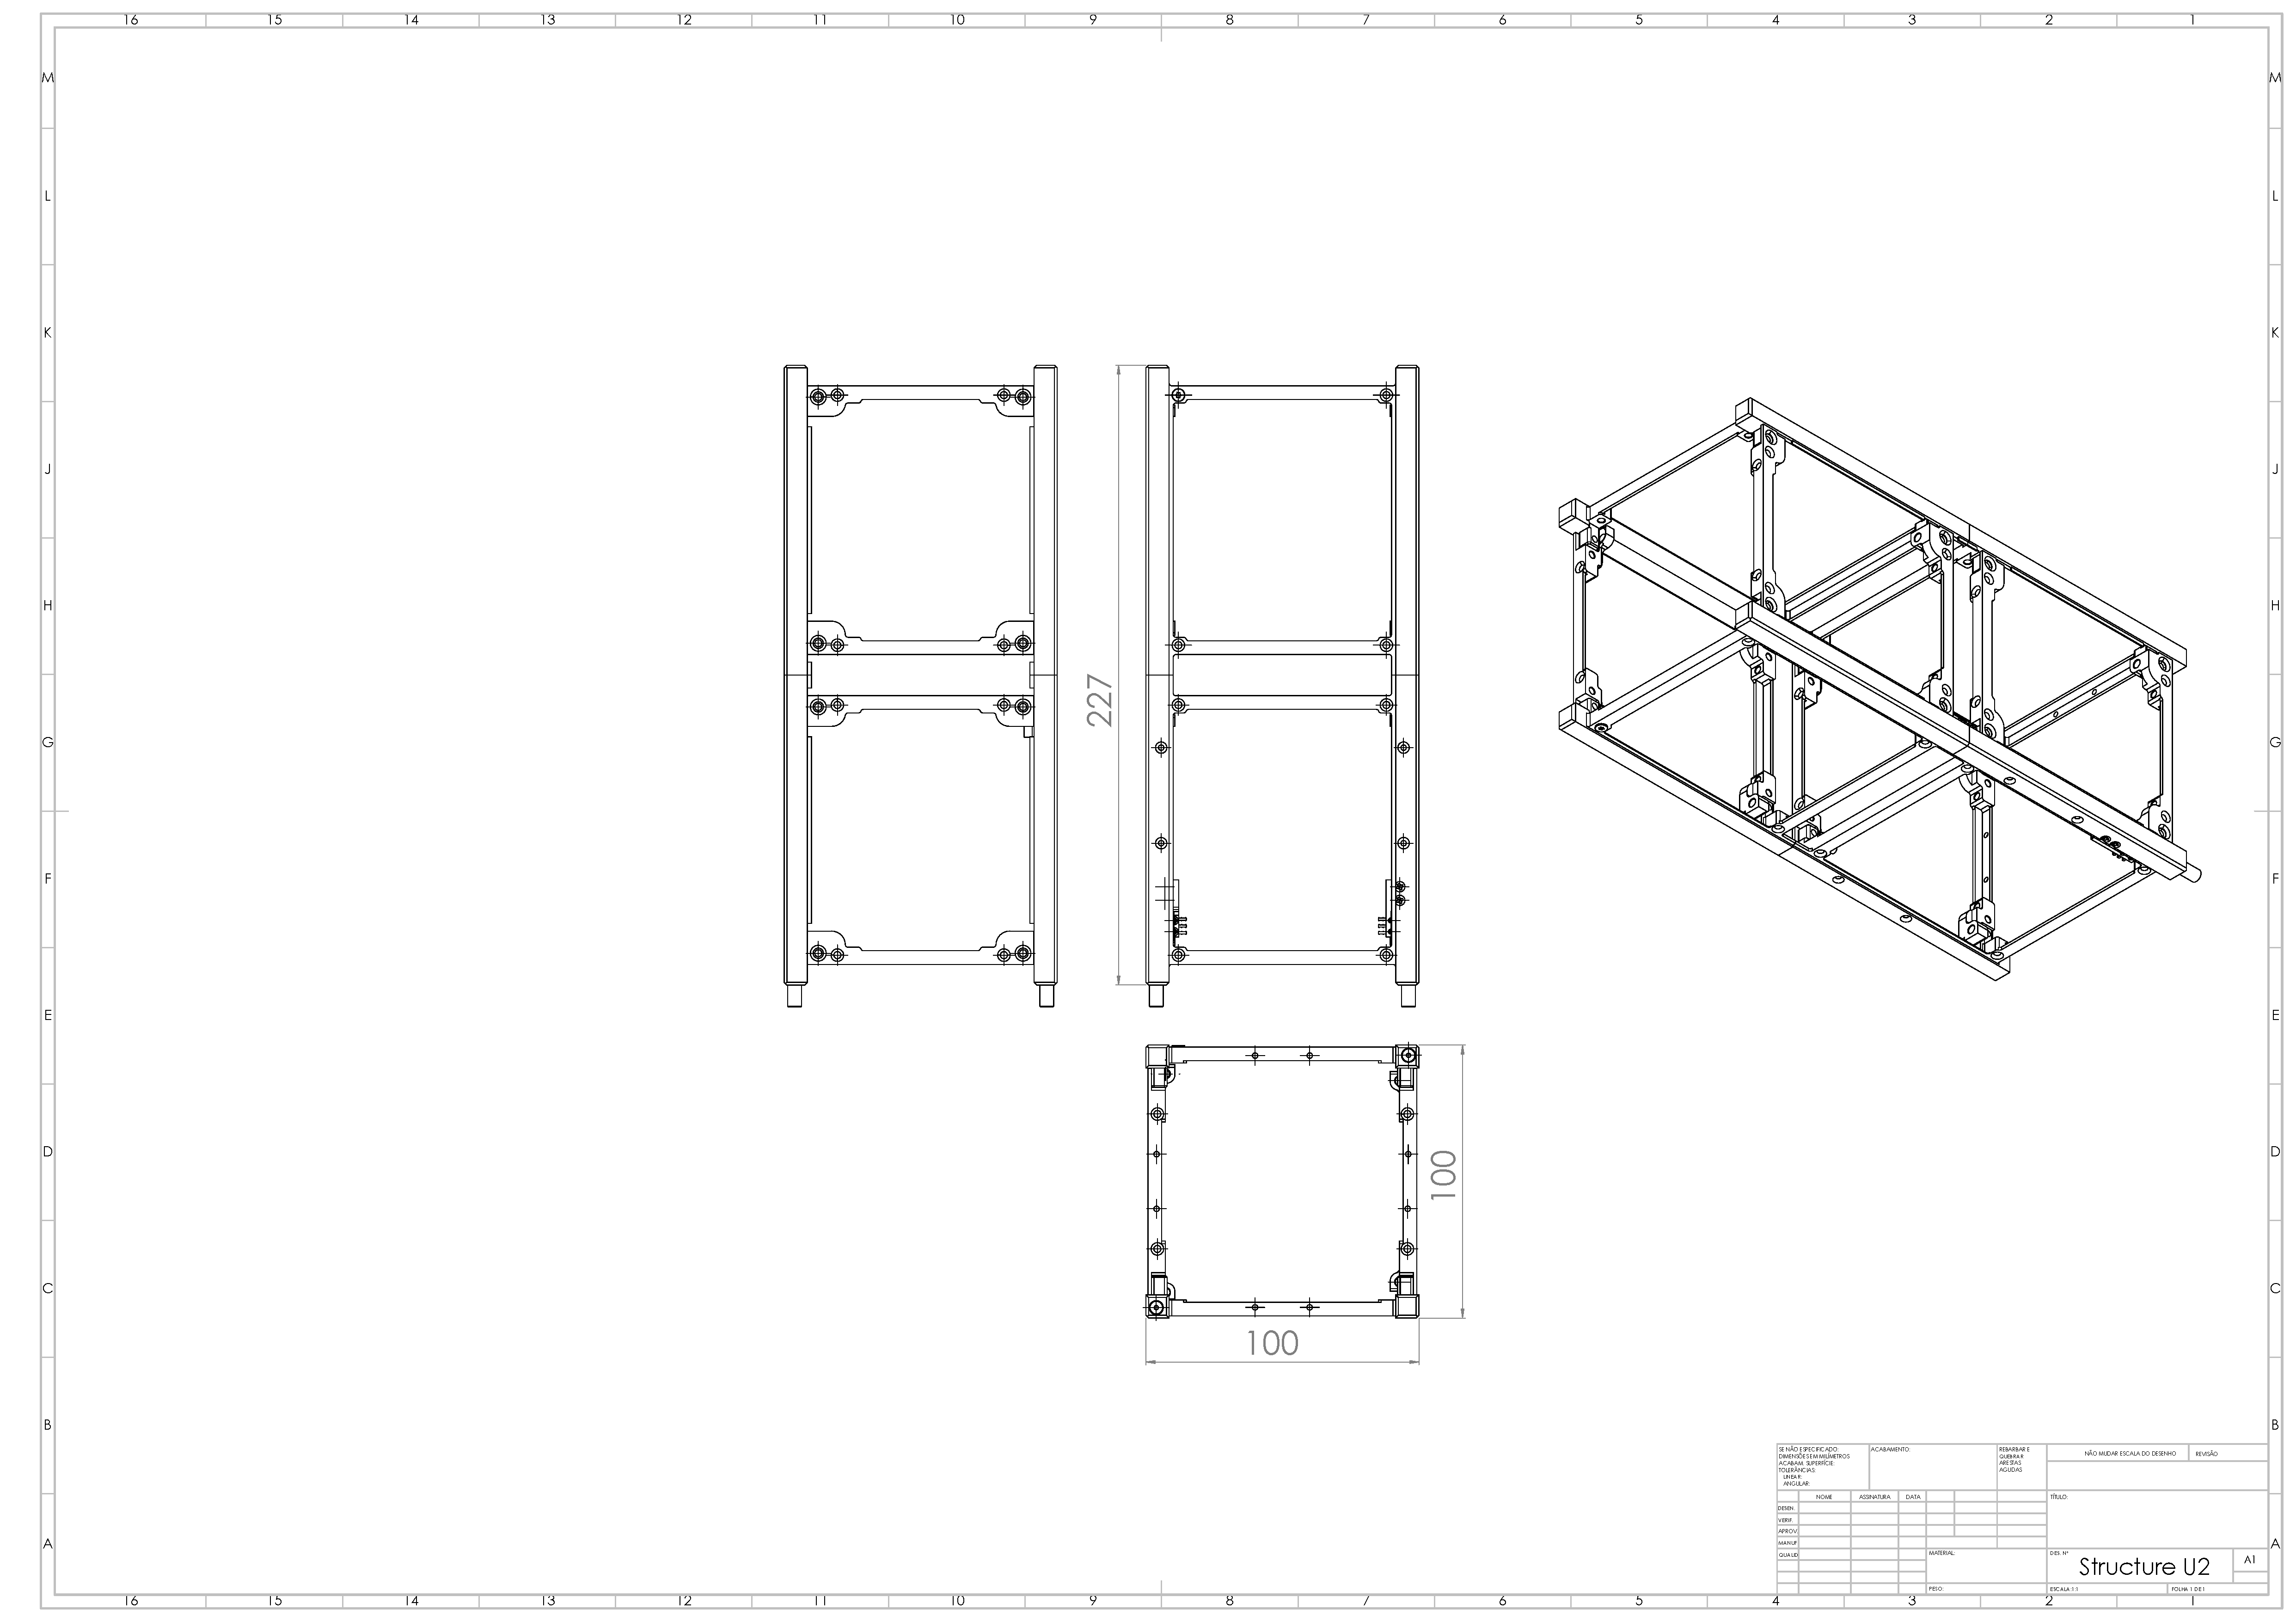
\includegraphics[width=0.8\textwidth, trim=25cm 8cm 30cm 13cm, clip=true]{figures/subsystems/Structure U2.pdf}
		\caption{Views and main dimension of the structure.}
		\label{fig:structure_views}
	\end{center}
\end{figure}

\section{ \textcolor{red}{TODO} Interconnection Modules}

\subsection{ \textcolor{red}{TODO} PC-104 Interconnection Boards}

The PC-104 interconnection boards are intended to be used as an interconnection of the two PC-104 bus segments of the 2U structure (top and bottom units). This interconnection is made with a set of PicoBlade cables between the top and bottom boards. The set of two boards can be seen in \autoref{fig:pc104-adapter}.

\begin{figure}[!ht]
    \begin{center}
        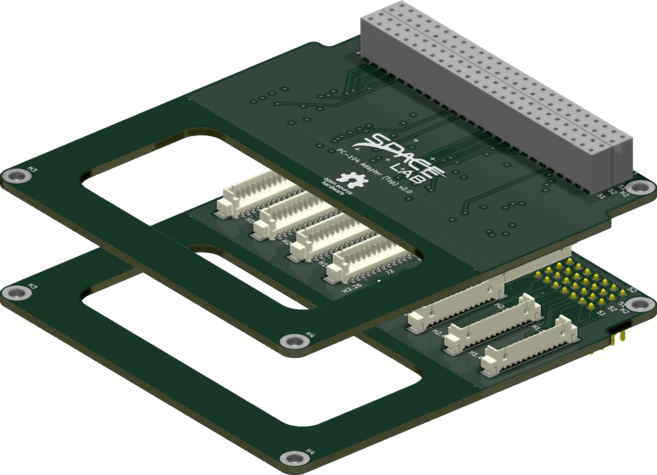
\includegraphics[width=0.7\textwidth]{figures/subsystems/pc104-adapter}
        \caption{PC-104 adapter boards (top and bottom).}
        \label{fig:pc104-adapter}
    \end{center}
\end{figure}

More information about these boards can be found in \cite{pc104-boards}.

\subsection{ \textcolor{red}{TODO} External Connection Boards}

The Interstage Interface Panels (IIP) are three vertical internally mounted PCBs designed to give external access to up to four modules inside of a 2U CubeSat during final assembly, integration, and testing (AIT) before launch. The complete set of boards allows the nanosatellite to be charged, programmed, and debugged. The usage of this hardware platform takes into account the use of a MSP-FET: MSP430 Flash Emulation Tool from Texas Instruments for JTAG programming and debugging, UART debugging through a mini USB type B port interfacing the FT4232H USB bridge IC from FTODOI, a JST XH header for charging internal batteries and a Remove Before Flight (RBF) pin header. The boards can be seen in \autoref{fig:iip-boards}.

\begin{figure}[!ht]
    \begin{center}
        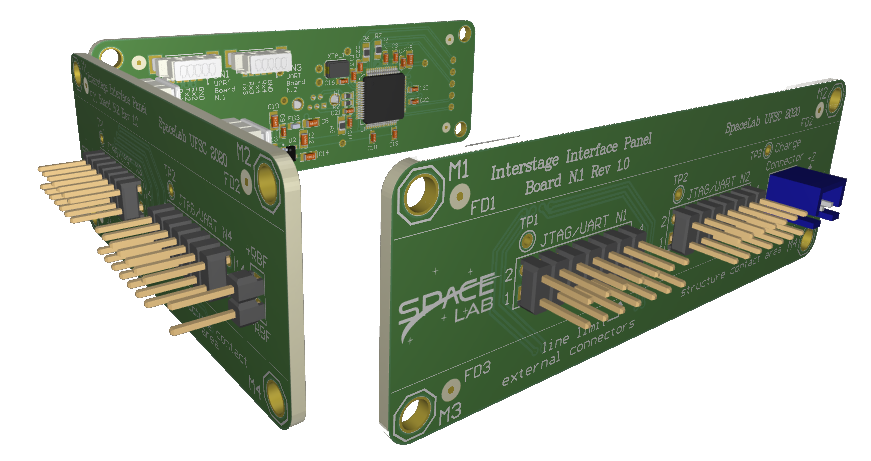
\includegraphics[width=0.7\textwidth]{figures/subsystems/iip_fullset}
        \caption{Set of external connection boards.}
        \label{fig:iip-boards}
    \end{center}
\end{figure}

For this mission, the four JTAG connectors are being used as described in \autoref{tab:iip-jtag-usage}.

\begin{table}[!h]
    \centering
    \begin{tabular}{lcccc}
        \toprule[1.5pt]
        \textbf{JTAG Connector} & \textbf{Connected Module} \\
        \midrule
        JTAG/UART N1 & OBDH \\
        JTAG/UART N2 & EPS \\
        JTAG/UART N3 & TTC \\
        JTAG/UART N4 & None \\
        \bottomrule[1.5pt]
    \end{tabular}
    \caption{IIP JTAG connectors usage.}
    \label{tab:iip-jtag-usage}
\end{table}

More information about these boards can be found in \cite{iip}.

\section{ \textcolor{red}{TODO} Payloads}

The Radio Occultation satellite is planned to carry the ``\textit{EDC}'' as the primary and main payload. Moreover, in order to asses the radiation levels present in the satellite, an additional scientific experiment is planned in the form of a Radiation instrument. Each one of these payloads are presented next.

\subsection{ \textcolor{red}{TODO} Environmental Data Collection}

The Environmental Data Collector (EDC\nomenclature{\textbf{EDC}}{\textit{Environmental Data Collection}.}) is a CubeSat-compatible payload that decodes signals from Platform Transmitter Terminals (PTTs) belonging to the Brazilian Environmental Data Collection System (SBCD\nomenclature{\textbf{SBCD}}{\textit{Sistema Brasileiro de Coleta de Dados}.}) and the Argos-2 System. It is the main payload of the Radio Occultation mission.

The main features of this payload are listed below, a 3D model of the EDC board can be seen in \autoref{fig:edc-board}.

\begin{itemize}
    \item Reception/decoding of SBCD and Argos-2 signals on the 401.635 MHz $\pm$ 30 kHz frequency range.
    \item Can decode up to 12 PTT signals simultaneously.
    \item Attaches a header to decoded messages with frequency, time, and signal strength information.
    \item Full speed I$^{2}$C interface (400 kbit/s) for the OBC communication.
    \item Full-duplex RS-485 interface with fail-safe for the OBC communication.
    \item 5 V power supply.
    \item Memory capable of storing up to 64 decoded user messages.
    \item Generates housekeeping information, including current supply, board temperature, digitized signal RMS level, front-end PLL synchronism state, and overcurrent events.
    \item Can capture a 2048 sample sequence (16 ms window) from the received signal upon request.
\end{itemize}

\begin{figure}[!ht]
    \begin{center}
        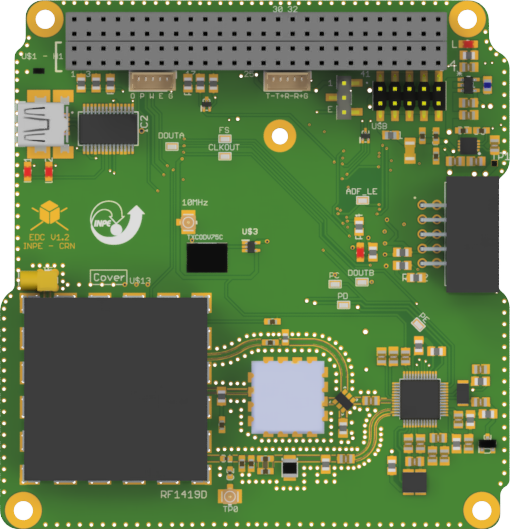
\includegraphics[width=0.6\textwidth]{figures/subsystems/edc-pcb-top}
        \caption{EDC board.}
        \label{fig:edc-board}
    \end{center}
\end{figure}

% As seen in \autoref{fig:exploded-view}, 
Two identical EDC boards will be used in a cold redundancy configuration for this mission. More information about this payload can be found in \cite{edc}.

\section{ \textcolor{red}{TODO} Radiation instrument}

The Radiation instrument is a radiation-hardened reconfigurable hardware platform designed for a radioactive environment, having as the main feature the possibility to change the hardware configuration of the FPGA\nomenclature{\textbf{FPGA}}{\textit{Field-Programmable Gate Array.}} through remote uplink of its bitstream.

\begin{figure}[!ht]
    \begin{center}
        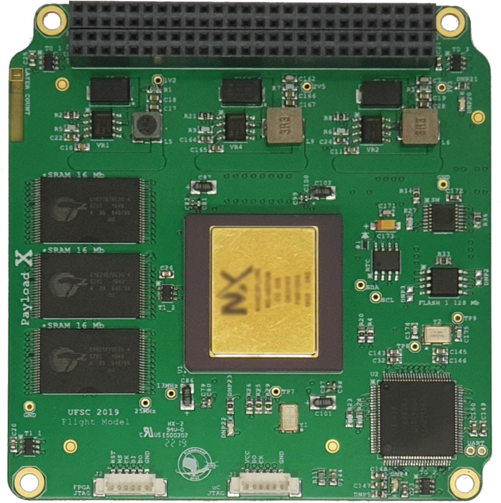
\includegraphics[width=0.6\textwidth]{figures/subsystems/payload-x-board}
        \caption{Radiation instrument board.}
        \label{fig:payload-x-board}
    \end{center}
\end{figure}

More information about this payload can be found in \cite{rigo2019}.

%\subsection{ \textcolor{red}{TODO} Radiation Monitor (Harsh Payload)}

%The Radiation Monitor (or Harsh Payload) is a payload capable of evaluate the radiation effects on three SDRAM\nomenclature{\textbf{SDRAM}}{\textit{Synchronous Dynamic Random-Access Memory.}} memories with different manufacturing nodes. This payload will test these chips in a harsh space environment by flying aboard the Radio Occultation CubeSat mission. These particular SDRAM memories were previously characterized in laboratory experiments. Exposing them to the real environments and executing the same test routines will not only generate more analysis results but also provide an opportunity to assess the test methodologies themselves. Also, after collecting sufficient data to be analyzed, this payload could be used to provide a meaningful health status concerning the radiation doses to which the satellite were exposed to the entire satellite subsystems and further missions. A picture of the harsh payload board is available in \autoref{fig:harsh-payload}.

%\begin{figure}[!ht]
%    \begin{center}
%        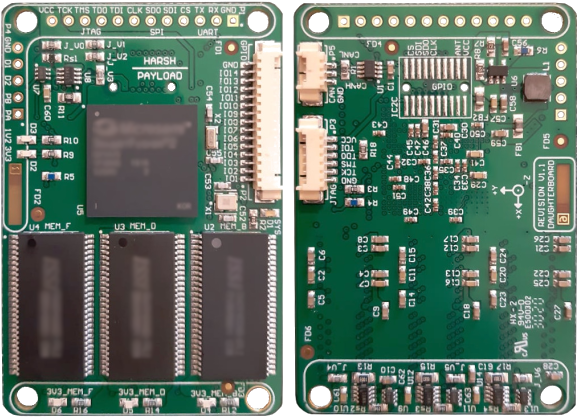
\includegraphics[width=0.7\textwidth]{figures/subsystems/harsh-payload}
%        \caption{Radiation monitor board. Top (left) and bottom (right) sides.}
%        \label{fig:harsh-payload}
%    \end{center}
%\end{figure}

%In order to accomplish this objectives, the payload is designed to follow the OBDH DaughterBoard standard of SpaceLab, which defines the connectors, shape and size of the board. This standard allows the utilization of the module throughout future SpaceLab core missions in reason of its low space occupation inside the CubeSat, being considered further as an expansion module instead of a payload experiment. A picture of the exploded view of the harsh payload and the OBDH can be seen in \autoref{fig:harsh-payload-integration}.

%\begin{figure}[!ht]
%    \begin{center}
%        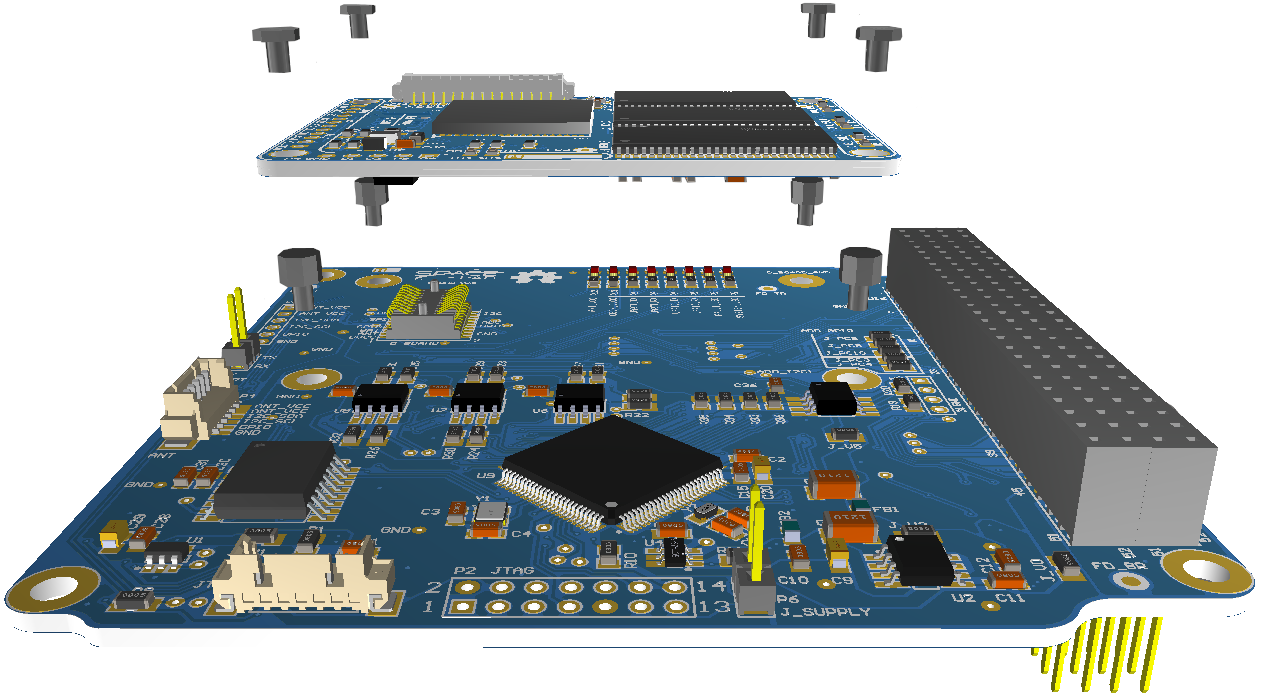
\includegraphics[width=0.7\textwidth]{figures/subsystems/daughterboard-integration}
%        \caption{Integration of the radiation monitor payload in the OBDH.}
%        \label{fig:harsh-payload-integration}
%    \end{center}
%\end{figure}

%Also, due to the limited power budget, the developed board should consider reducing power consumption and defining clever power management strategies. In addition, methods for anti latch-up, a type of short circuit which can occur inside an IC, are considered in the design. Therefore, combining all these requirements, the payload architecture consists of the following modules: a control and management subsystem, operated by a System-On-a-Chip (SoC\nomenclature{\textbf{SoC}}{\textit{System-On-a-Chip.}}) solution with an integrated FPGA, power converters for properly voltage level supply, anti latch-up circuitry, communication and interface buses, debug module and the SDRAM memory chips.

    %
% ground_segment.tex
%
% Copyright The Radio Occultation Contributors.
%
% Radio Occultation Documentation
%
% This work is licensed under the Creative Commons Attribution-ShareAlike 4.0
% International License. To view a copy of this license,
% visit http://creativecommons.org/licenses/by-sa/4.0/.
%

%
% \brief Ground segment chapter.
%
% \author Gabriel Mariano Marcelino <gabriel.mm8@gmail.com>
%
% \version 0.2.0
%
% \date 2020/06/06
%

\chapter{ \textcolor{red}{TODO} Ground Segment} \label{ch:ground-segment}

This chapter describes the ground segment of the mission. It is composed of two ground stations (one at the INPE-RN installations and the other at the SpaceLab installations) and many data collection platforms (PCD\nomenclature{\textbf{PCD}}{\textit{``Plataforma de Coleta de Dados'', or Data Collection Platform}}, or \textit{``Plataforma de Coleta de Dados''}), installed at a variety of locations on the Brazilian territory.

The control of the mission and the reception of the collected data will be performed mainly at these two ground stations, but if necessary, other stations can execute this task. Any station in the world can use the amateur radio link since having the required equipment to it.

\section{ \textcolor{red}{TODO} UFSC Ground Station}

The UFSC ground station is currently being developed and prepared for this mission. This section presents the project of this station. A general block diagram can be seen in \autoref{fig:grs-block-diagram}.

\begin{figure}[!ht]
    \begin{center}
        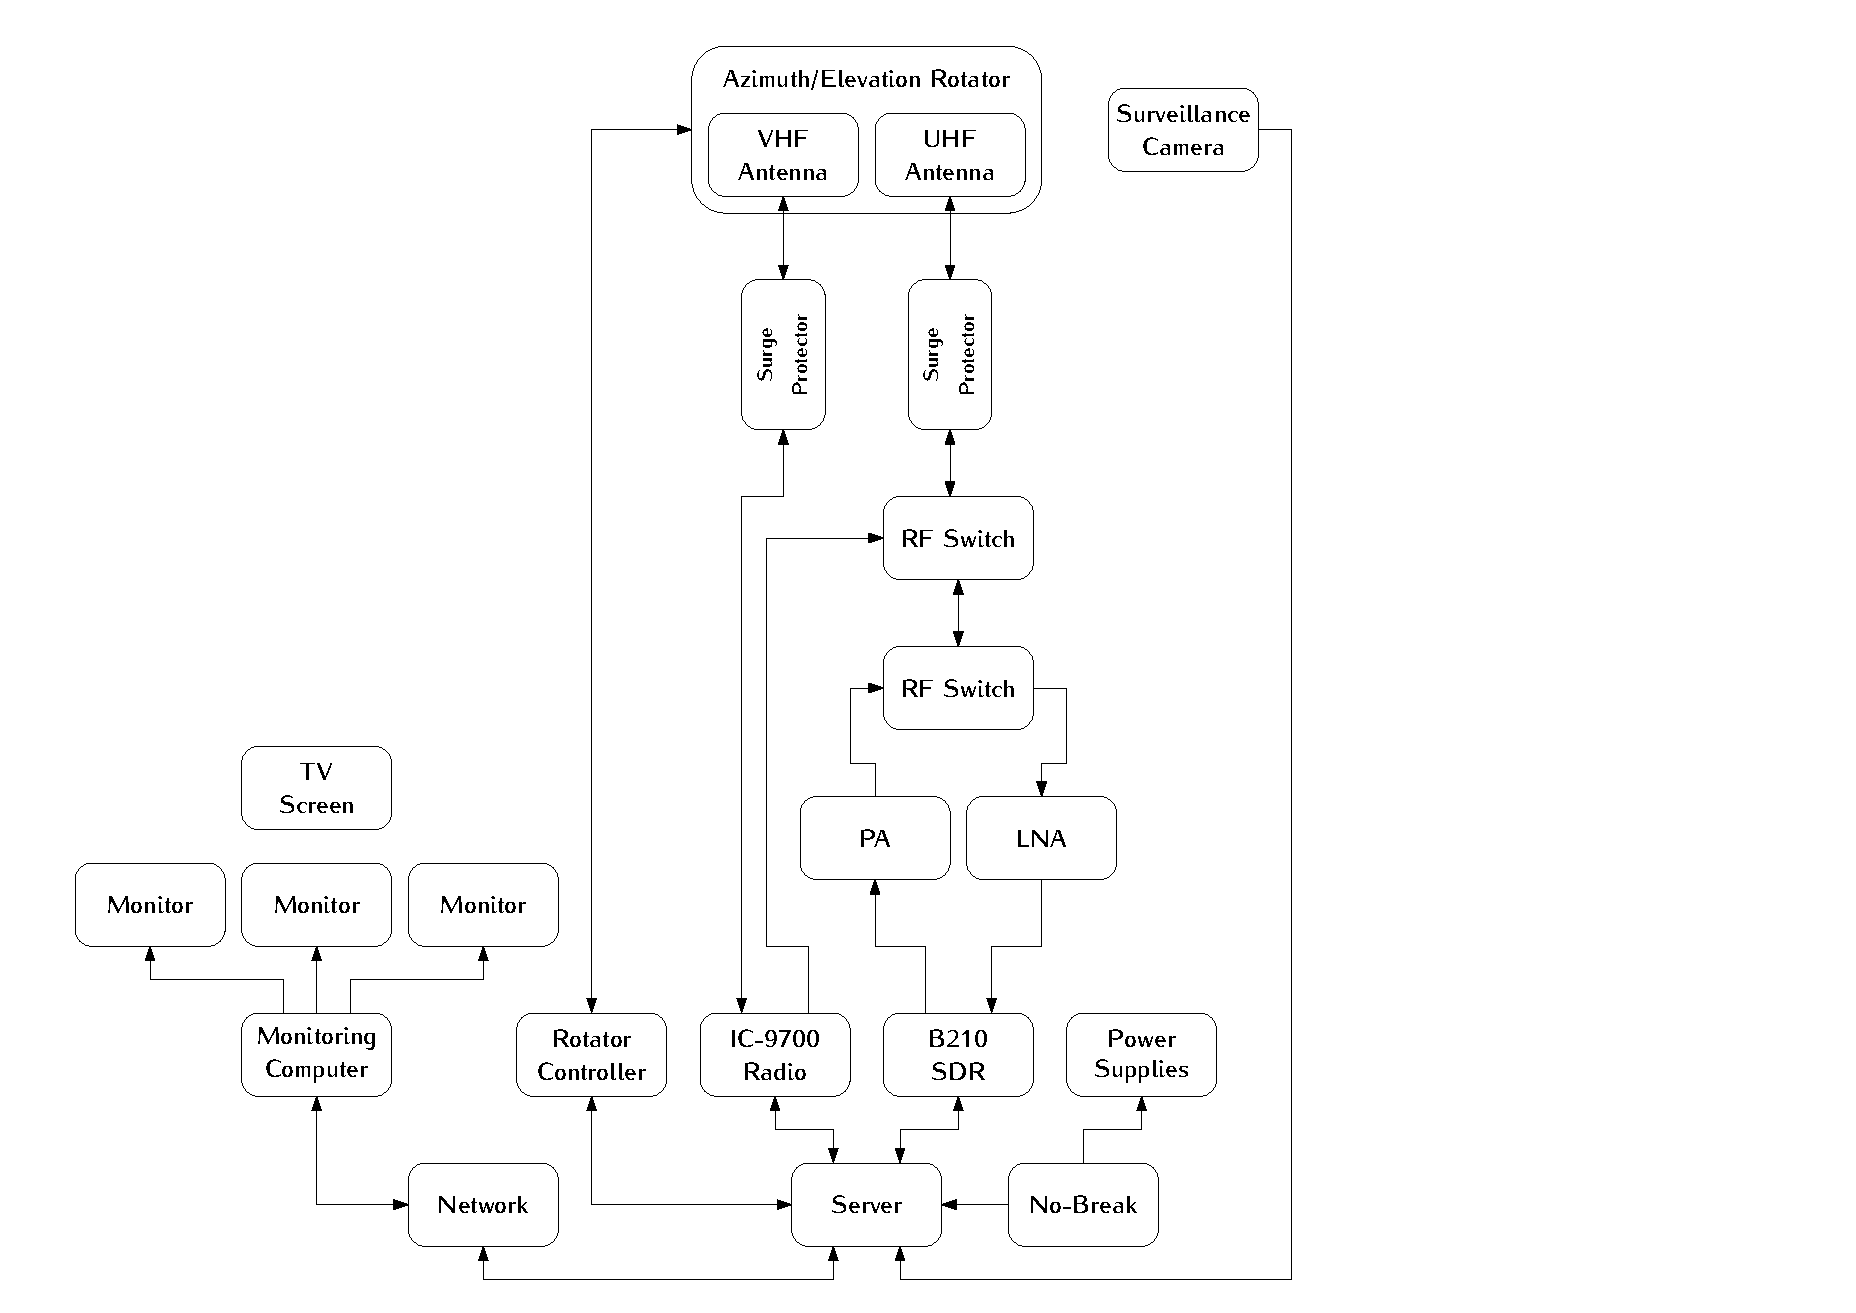
\includegraphics[width=\textwidth]{figures/grs-block-diagram.pdf}
        \caption{Block diagram of the ground segment (UFSC ground station).}
        \label{fig:grs-block-diagram}
    \end{center}
\end{figure}

In the following sections, a description of the main components of the station will be presented.

\subsection{ \textcolor{red}{TODO} Hardware}

This part describes the hardware side of the UFSC ground station and details the main peripherals that will be used in this project. Most of the components described here are represented in \autoref{fig:grs-block-diagram}.

\subsubsection{Antennas}

There are two antennas in the ground station: One for VHF and one for the UHF band. The main characteristics of these antennas can be seen in \autoref{tab:grs-antennas}

\begin{table}[ht]
    \centering
    \begin{tabular}{lccc}
        \toprule[1.5pt]
        \textbf{Characteristic} & \textbf{VHF Antenna}  & \textbf{UHF Antenna}  & \textbf{Unit} \\
        \midrule
        Brand                   & M$^{2}$               & Cushcraft             & - \\
        Model                   & 2MCP14                & A719B                 & - \\
        Type                    & Yagi                  & Yagi                  & - \\
        Number of elements      & 14                    & 19                    & - \\
        Frequency range         & 143-148               & 430-450               & MHz \\
        Gain                    & 12.34                 & 15.5                  & dBi \\
        Power rating            & 1500                  & 2000                  & W \\
        Boom length             & 3.2                   & 4.1                   & m \\
        Longest element         & 1.02                  & 0.34                  & m \\
        Weight                  & 2.72                  & 2.55                  & kg \\
        \bottomrule[1.5pt]
    \end{tabular}
    \caption{Main characteristics of the ground segment antennas.}
    \label{tab:grs-antennas}
\end{table}

More information about the VHF and UHF antennas can be found in \cite{2mcp14} and \cite{a719b} respectively.

\paragraph{Surge Protector}

Two surge protectors will be used to protect the ground station electronics of possible atmospheric discharges in the outside components (one for each antenna). The gas surge protectors safely discharge/deflect up to 5000 A of peak current to earth without causing damage to an independent ground. This device is installed near the antennas, in cascade with the RF cables.

For this project, the model MFJ-270N will be used, and a picture of it can be seen in \autoref{fig:mfj-270n}.

\begin{figure}[!ht]
    \begin{center}
        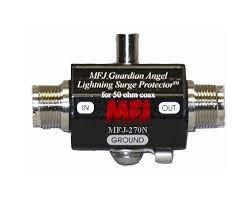
\includegraphics[width=0.4\textwidth]{figures/mfj-270n.jpeg}
        \caption{MFJ-270N surge protector.}
        \label{fig:mfj-270n}
    \end{center}
\end{figure}

\subsubsection{Rotators}

Both antennas (VHF and UHF) track the satellite through a two axis rotator (azimuth and elevation). The used model is the Yaesu G-5500, which provides 450$^{\circ}$ azimuth and 180$^{\circ}$ elevation control of medium and large size unidirectional satellite antenna arrays under remote control from station operation position.

A picture of the G-5500 rotator (and controller) can be seen in \autoref{fig:g5500}; the main characteristics can be found in \autoref{tab:grs-rotor}.

\begin{figure}[!ht]
    \begin{center}
        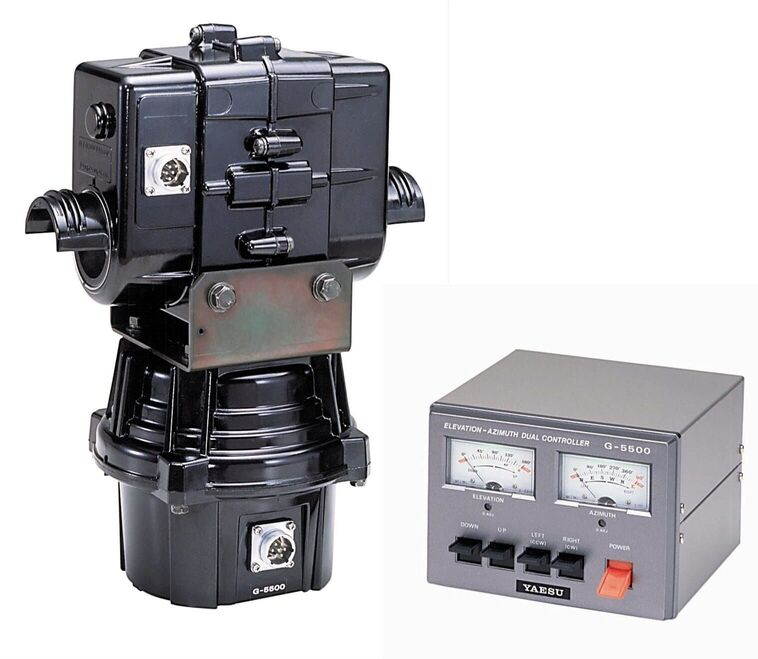
\includegraphics[width=0.6\textwidth]{figures/g5500.jpg}
        \caption{Yaesu G-5500 rotator and controller.}
        \label{fig:g5500}
    \end{center}
\end{figure}

\begin{table}[ht]
    \centering
    \begin{tabular}{lcc}
        \toprule[1.5pt]
        \textbf{Characteristic}                     & \textbf{Value}        & \textbf{Unit} \\
        \midrule
        Brand                                       & Yaesu                 & - \\
        Model                                       & G-5500                & - \\
        Voltage requirement                         & 110-120 or 200-240    & $V_{AC}$ \\
        Motor voltage                               & 24                    & V$_{AC}$ \\
        Rotation time (elevation, 180$^{\circ}$)    & 67                    & s \\
        Rotation time (azimuth, 360$^{\circ}$)      & 58                    & s \\
        Maximum continuous operation                & 5                     & min \\
        Rotation torque (elevation)                 & 14                    & kg-m \\
        Rotation torque (azimuth)                   & 6                     & kg-m \\
        Braking torque (elevation and azimuth)      & 40                    & kg-m \\
        Vertical load                               & 200                   & kg \\
        Pointing accuracy                           & $\pm$ 4               & \% \\
        Wind surface area                           & 1                     & $m^{2}$ \\
        Weight (rotator)                            & 9                     & kg \\
        Weight (controller)                         & 3                     & kg \\
        \bottomrule[1.5pt]
    \end{tabular}
    \caption{Main characteristics of antennas' rotators.}
    \label{tab:grs-rotor}
\end{table}

More information about the ground station rotator can be found in \cite{g5500}.

\subsubsection{Amplifiers}

There are two dedicated amplifiers in the UFSC ground station: one power amplifier (PA) for transmitting telecommands with a high power signal, and a low noise amplifier (LNA), for amplify the received signals from the satellite. Both are presented next.

\paragraph{Power Amplifier}

The power amplifier is used to add a gain to the generated signals of the transmitter. The used model is the Mini-Circuits ZHL-50W-52-S+ \cite{zhl50w}. A picture of this power amplifier can be seen in \autoref{fig:zhl-50w}, the main characteristics are available in \autoref{tab:zhl-50w-specs}.

\begin{figure}[!ht]
    \begin{center}
        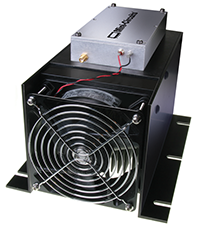
\includegraphics[width=0.3\textwidth]{figures/zhl-50w.png}
        \caption{Mini-Circuits ZHL-50W-52-S+ power amplifier.}
        \label{fig:zhl-50w}
    \end{center}
\end{figure}

\begin{table}[ht]
    \centering
    \begin{tabular}{lcc}
        \toprule[1.5pt]
        \textbf{Characteristic} & \textbf{Value}    & \textbf{Unit} \\
        \midrule
        Brand                   & Mini-Circuits     & - \\
        Model                   & ZHL-50W-52-S+     & - \\
        Frequency range         & 50-500            & MHz \\
        Gain                    & 47-52             & dB \\
        Noise figure            & 4.5-7.0           & dB \\
        DC supply voltage       & 24-25             & V \\
        Max. supply current     & 9.3               & A \\
        \bottomrule[1.5pt]
    \end{tabular}
    \caption{Main characteristics of the ZHL-50W-52-S+ power amplifier.}
    \label{tab:zhl-50w-specs}
\end{table}

\paragraph{Low Noise Amplifiers}

As LNA, the model ZFL-500LN+ from Mini-Circuits \cite{zfl500ln} is being used. This amplifier will be used just after the antennas to add a gain to the incoming telemetry signals transmitted by the satellite. A picture of the low noise amplifier can be seen in \autoref{fig:lna}, the main characteristics are available in \autoref{tab:lna-specs}.

\begin{figure}[!ht]
    \begin{center}
        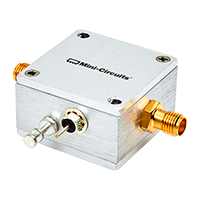
\includegraphics[width=150pt]{figures/lna.png}
        \caption{Mini-Circuits ZFL-500LN+ low noise amplifier.}
        \label{fig:lna}
    \end{center}
\end{figure}

\begin{table}[ht]
    \centering
    \begin{tabular}{lcc}
        \toprule[1.5pt]
        \textbf{Characteristic} & \textbf{Value}    & \textbf{Unit} \\
        \midrule
        Brand                   & Mini-Circuits     & - \\
        Model                   & ZFL-500LN+        & - \\
        Frequency range         & 0.1-500           & MHz \\
        Gain                    & 24-28             & dB \\
        DC supply voltage       & 15                & V \\
        Max. supply current     & 60                & mA \\
        \bottomrule[1.5pt]
    \end{tabular}
    \caption{Main characteristics of the ZFL-500LN+ low noise amplifier.}
    \label{tab:lna-specs}
\end{table}

\subsubsection{Radios}

Besides the SDR solution presented in the block diagram of the \autoref{fig:grs-block-diagram}, there is also a amateur radio transceiver with a standalone solution for the amateur radio link with the satellite. The used model is the Icom IC-9700 \cite{ic9700}, that is an RF direct sampling receiver for 2 m and 70 cm. The IF receiver consists of a single down conversion for 23 cm that is between 311 and 371 MHz. The PA provides 100 W on 2 m, 75 W on 70 cm, and 10 W on 23 cm.

In addition to band-specific memory channels, the IC-9700 allows the band-specific receiver and transmitter settings. For transmission, users can adjust RF power, TX power Limit, Limit Power, and TX Delay by the band. Basic receiver settings, like the Noise Blanker, Noise Reduction, and others, can be tweaked by the band with a dynamic Notch and Filter setup by band/mode. A picture of the IC-9700 radio can be seen in \autoref{fig:ic9700}.

\begin{figure}[!ht]
    \begin{center}
        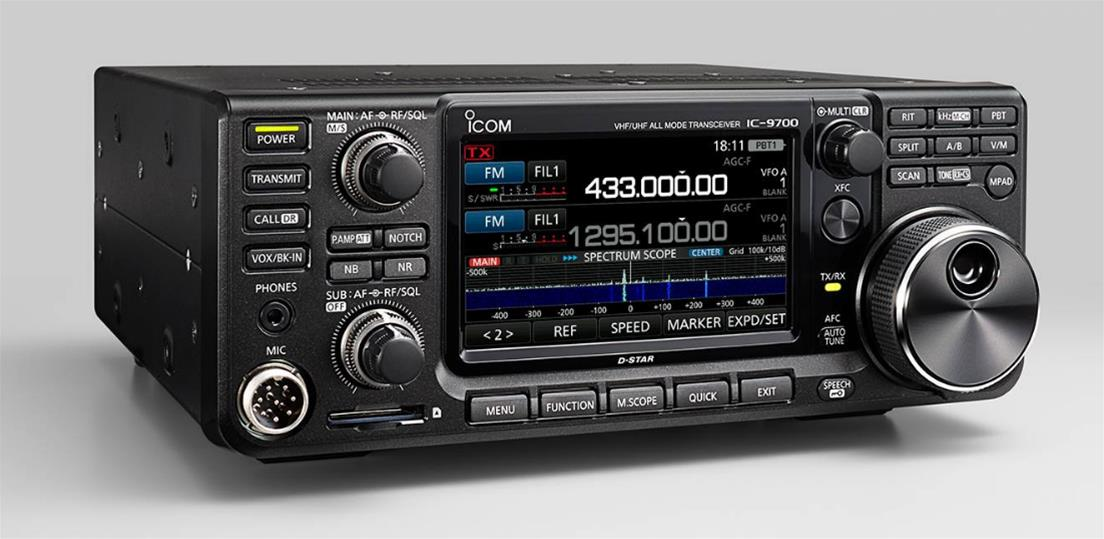
\includegraphics[width=0.7\textwidth]{figures/ic-9700.jpg}
        \caption{Icom IC-9700 radio transceiver.}
        \label{fig:ic9700}
    \end{center}
\end{figure}

\paragraph{Software Defined Radio}

As presented in \autoref{fig:grs-block-diagram}, the ground segment also has an SDR\nomenclature{\textbf{SDR}}{\textit{Software Defined Radio.}} (Software Defined Radio) as a transceiver. The used model is the USRP B210, from Ettus Research \cite{b210}, a fully integrated, single-board SDR with continuous frequency coverage from 70 MHz to 6 GHz. It combines the AD9361 RFIC direct-conversion transceiver providing up to 56 MHz of real-time bandwidth, an open and reprogrammable Spartan6 FPGA, and USB 3.0 connectivity. Also, full support for the USRP Hardware Driver (UHD) software allows the use of the GNURadio framework. A picture of the USRP B210 SDR (with enclosure) can be seen in \autoref{fig:usrp-b210}.

\begin{figure}[!ht]
    \begin{center}
        \includegraphics[width=0.6\textwidth]{figures/usrp-b210.jpg}
        \caption{Ettus USRP B210 SDR.}
        \label{fig:usrp-b210}
    \end{center}
\end{figure}

\subsubsection{Processing and Control}

The ground station control room shall have two monitors and a dedicated computer alongside most of the previously presented hardware. It will work as a monitoring room with a nobreak to protect the equipment from power grid fluctuations. 

The antennas and rotator will also be monitored with outside cameras. And the room will count with a server so that the transmission and decoding can be done remotely and at any time.

In the \autoref{fig:server} can be seen a picture of the used server, and in \autoref{tab:server} are presented the main characteristics of the it.

\begin{table}[ht]
    \centering
    \begin{tabular}{lc}
        \toprule[1.5pt]
        \textbf{Characteristic} & \textbf{Value} \\
        \midrule
        Brand                   & Dell \\
        Model                   & PowerEdge R240 \\
        Processor               & Intel Xeon E-2244G 3.8 GHz 4C/8T \\
        RAM Memory              & 16 GB DDR4 ECC \\
        Storage                 & 1 TB HD \\
        \bottomrule[1.5pt]
    \end{tabular}
    \caption{Main characteristics of the Dell PowerEdge R240 server.}
    \label{tab:server}
\end{table}

\begin{figure}[!ht]
    \begin{center}
        \includegraphics[width=300pt]{figures/server.jpg}
        \caption{Dell PowerEdge R240 server.}
        \label{fig:server}
    \end{center}
\end{figure}

\subsection{ \textcolor{red}{TODO} Satellite Tracking}

To track the satellite and for orbit prediction, the GPredict software \cite{gpredict} will be used. Gpredict is a real-time satellite tracking and orbit prediction application. It can track many satellites and display their position and other data in lists, tables, maps, and polar plots (radar view). Gpredict can also predict the time of future passes for a satellite and provide detailed information about each pass. Gpredict is free software licensed under the GNU General Public License. A picture of the main window of GPredict can be seen in \autoref{fig:gpredict}.

\begin{figure}[!ht]
    \begin{center}
        \includegraphics[width=\textwidth]{figures/gpredict.png}
        \caption{Main window of GPredict.}
        \label{fig:gpredict}
    \end{center}
\end{figure}

\subsection{ \textcolor{red}{TODO} Packet Transmission}

The packet generation and transmission to Radio Occultation satellite can be done with the SpaceLab-Transmitter software \cite{spacelab-transmitter}, which was written in Python with the interface developed using the GTK framework. It has a USRP Handler made with Ettus libraries to work with Ettus USRP B210 as shown in \autoref{fig:usrp-b210}. The supported modulation is the Gaussian Minimum Shift Keying (GMSK). Furthermore, the software also has unit tests for the main modules and a logging system to record events such as an initialization or a successfully transmitted telecommand.

In the \autoref{fig:transmitter-tree} is shown the product tree of the software, which contains its main elements of it, and in the \autoref{fig:spacelab-transmitter} is shown the main window of it.

\begin{figure}[!ht]
    \begin{center}
        \includegraphics[width=0.6\textwidth]{figures/transmitter_tree.pdf}
        \caption{SpaceLab-Transmitter product tree.}
        \label{fig:transmitter-tree}
    \end{center}
\end{figure}

\begin{figure}[!ht]
    \begin{center}
        \includegraphics[width=\textwidth]{figures/spacelab-transmitter-window.png}
        \caption{Main window of the SpaceLab-Transmitter application.}
        \label{fig:spacelab-transmitter}
    \end{center}
\end{figure}

\subsection{ \textcolor{red}{TODO} Packet Decoding}

The packet decoding of Radio Occultation satellites telemetry can be done using the SpaceLab-Decoder \cite{spacelab-decoder} software using a .wav file or through a real time reception. The decoded telemetry will appear in a dialog within the main window. The software was written in Python, and the interface was developed using GTK framework. Furthermore, the software also has unit tests for the main modules and a logging system to record events.

The \autoref{fig:decoder-tree} is showing the product tree of the software, which contains its main elements, and in the \autoref{fig:spacelab-transmitter} is shown the main window of it.

\begin{figure}[!ht]
    \begin{center}
        \includegraphics[width=0.6\textwidth]{figures/decoder_tree.pdf}
        \caption{SpaceLab-Decoder product tree.}
        \label{fig:decoder-tree}
    \end{center}
\end{figure}

\begin{figure}[!ht]
    \begin{center}
        \includegraphics[width=\textwidth]{figures/spacelab-decoder.png}
        \caption{Main window of the SpaceLab-Decoder application.}
        \label{fig:spacelab-decoder}
    \end{center}
\end{figure}

\section{ \textcolor{red}{TODO} EMMN Ground Station}

The EMMN\nomenclature{\textbf{EMMN}}{\textit{Estação Mutlimissão de Natal.}} (\textit{Estação Multimissão de Natal} in portuguese) ground station \cite{emmn} was designed to operate in VHF, UHF and S-Band frequency bands, receiving payload and telemetry data and transmitting telecommands from and to satellites operating in low orbits.

The station's radio frequency systems use Software Defined Radios (SDRs), which offer the flexibility to quickly reconfigure parameters such as modulation type, encoding, datarate, etc. Most commonly used modulation schemes and encoding methods are already implemented, and any customization requests can be requested.

The station performs autonomous tracking of several satellites according to a previous schedule and a scale of priorities. A Client-Server network design allows station users to send and receive data remotely.

A general block diagram of the EMMN hardware is available in \autoref{fig:emmn-bd}.

\begin{figure}[!ht]
    \begin{center}
        \includegraphics[width=\textwidth]{figures/emmn-bd}
        \caption{General block diagram of the EMMN.}
        \label{fig:emmn-bd}
    \end{center}
\end{figure}

\begin{table}[!h]
    \centering
    \begin{tabular}{lC{6cm}}
        \toprule[1.5pt]
        \textbf{Parameter} & \textbf{Value} \\
        \midrule
        Grid locator    & HI24JD59CI \\
        Coordinates     & -5.835238, -35.209285 \\
        Altitude        & 51 m \\
        Antennas        & Yagi and parabolic \\
        Bands           & VHF, UHF and S-Band\\
        Frequencies     & 144-146 MHz (VHF), 395-405 and 432-440 MHz (UHF) 2200-3300 MHz (S-Band)\\
        \bottomrule[1.5pt]
    \end{tabular}
    \caption{EMMN specs.}
    \label{tab:emmn-info}
\end{table}

\begin{figure}[!ht]
    \begin{center}
        \includegraphics[width=\textwidth]{figures/inpe-emmn}
        \caption{Multimission station of Natal-RN.}
        \label{fig:emmn}
    \end{center}
\end{figure}

\section{ \textcolor{red}{TODO} Data Collection Platforms}

Data Collection Platforms (DCPs) are part of the Integrated System of Environmental Data (\textit{Sistema Integrado de Dados Ambientais, SINDA} \cite{sinda}, in Portuguese), which collects the data and by satellites, it is retransmitted to be received in the ground station so that it can be sent to SINDA to be processed. The data is shown online sometime after the receiving. Examples of DCPs can be seen in \autoref{fig:dcp-ex}.

\begin{figure}[!htb]
    \begin{center}
        \subfigure[\label{fig:dcp-ex-1}]{\includegraphics[width=0.48\textwidth]{figures/pcd-1}}
        ~
        \subfigure[\label{fig:dcp-ex-2}]{\includegraphics[width=0.48\textwidth]{figures/pcd-2}}

        \subfigure[\label{fig:dcp-ex-2}]{\includegraphics[width=0.48\textwidth]{figures/pcd-3}}
        \caption{Examples of data collection platforms (DCPs).}
        \label{fig:dcp-ex}
    \end{center}
\end{figure}

    %
% tests.tex
%
% Copyright (C) 2021 by SpaceLab.
%
% Radio Occultation Documentation
%
% This work is licensed under the Creative Commons Attribution-ShareAlike 4.0
% International License. To view a copy of this license,
% visit http://creativecommons.org/licenses/by-sa/4.0/.
%

%
% \brief Test plan and results.
%
% \author Gabriel Mariano Marcelino <gabriel.mm8@gmail.com>
%
% \institution Universidade Federal de Santa Catarina (UFSC)
%
% \version 0.2.0
%
% \date 2021/01/21
%

\chapter{ \textcolor{red}{TODO} Test Plan and Procedures} \label{ch:test-plan}

The Radio Occultation test plan is structured into four phases: Module tests, FlatSat, Engineering integration, and Flight integration. This plan is summarized in the \autoref{tab:test-plan} and includes the components under test for each phase. 

\begin{table}[!h]
    \begin{center}
        \begin{tabular}{ll}
            \toprule[1.5pt]
            \textbf{Phase}    & \textbf{Components}       \\
            \midrule
            Module tests             & OBDH module \\
                                     & EPS module \\
                                     & TTC module \\
                                     & BATC4 board \\
                                     & IIP boards \\
                                     & PC104-ADPT boards \\
                                     & ACS components (simulation) \\
                                     & Mechanical (CAD assessment) \\
            \midrule
            FlatSat                  & Satellite core (OBDH+EPS+TTC+BATC4) \\
                                     & Satellite core + GRS \\
                                     & Satellite core + Payloads \\
                                     & Satellite core + Payloads + GRS \\
                                     & Satellite (long-term evaluation) \\
            \midrule
            Engineering integration  & Mechanical assembly (repeated when required) \\
            (clean room preferable)  & Satellite core + Payloads + GRS \\
                                     & Satellite (long-term evaluation) \\
                                     & Satellite + Solar Panels \\
                                     & Preliminary environmental tests \\ 
            \midrule
            Flight integration       & Mechanical assembly (flight components) \\
            (clean room mandatory)   & Satellite (short-term evaluation) \\
                                     & Satellite + Antenna (deployment) \\
                                     & Mechanical reassembly for flight \\
                                     & Satellite (long-term evaluation) \\
                                     & Qualification environmental tests \\ 
            \bottomrule[1.5pt]
        \end{tabular}
        \caption{Test plan phases and tested components.}
        \label{tab:test-plan}
    \end{center}
\end{table}

This section provides an overview of the planned testing workflow and a description of the strategies to accomplish the mission objectives. The module tests focus on the individual module's operation and behavior, in which a general template is provided in this document, and each module applies it for its needs. The FlatSat phase is the first module integration in a debug platform to validate the system from a development perspective (described with more details in \cite{flatsat}). Finally, the engineering integration is the final development campaign aiming to validate the system from a mission perspective. The flight integration is the actual CubeSat assembly using the flight components and final assessments to prepare the satellite for launch. The integration details, procedures, and qualification process are described with more depth in the \autoref{ch:ait}. % maybe it will be splitted in a separated document


\section{ \textcolor{red}{TODO} Module tests}

The first phase is the foundation for the satellite, consolidating the base design for each subsystem and shaping their relations. Therefore, several techniques were employed to ensure a solid test strategy: several inspections of the boards' design and manufacturing quality; manual experimental assessments of various hardware, electrical, mechanical, and behavioral parameters; remotely automated tests using a continuous integration (CI)\nomenclature{\textbf{CI}}{\textit{Continuos Integration.}} approach; semi-automated tests using a hardware-in-the-loop (HIL)\nomenclature{\textbf{HIL}}{\textit{Hardware-In-the-Loop.}} strategy; simulations; and CAD models assessment.

\subsection{ \textcolor{red}{TODO} Workflow}

The following topics list the template workflow used to create the procedures for each subsystem. Each module documentation has its test chapter describing the process in detail, from procedures to success criteria.

% \item [\footnotesize{XX-00}] Text 
\subsubsection{Visual Inspection} 
\begin{enumerate} \setlength\itemsep{-0.3em}
    \item Packaging quality assessment
    \item Board manufacturing and assembly quality
    \item 3D model comparison
    \item Layers marker
    \item Labels (schematics comparison) 
    \item High resolution photos for documentation
\end{enumerate}

\subsubsection{Mechanical Inspection}
\begin{enumerate} \setlength\itemsep{-0.3em}
    \item Board dimensions and mounting holes positioning
    \item Board weight measurement
\end{enumerate}

\subsubsection{Integration Inspection}
\begin{enumerate} \setlength\itemsep{-0.3em}
    \item Check connectors pinout against the documentation (not schematics)
    \item Check connectors positioning (if applicable)
\end{enumerate}

\subsubsection{Electrical Inspection}
\begin{enumerate} \setlength\itemsep{-0.3em}
    \item Solder shorts
    \item Missing components
    \item Lifted pins
    \item Poor soldering
    \item Swapped components
    \item Components part number
    \item Components polarity (schematic comparison)
    \item Components defined to not be soldered (DNP)
\end{enumerate}

\subsubsection{Electrical Testing}
\begin{enumerate} \setlength\itemsep{-0.3em}
    \item Continuity test
    \item Power up procedures (check LEDs and test points)
    \item Average input power consumption measurement
    \item Average output power source measurement (if applicable) 
    \item Power tracks temperature (if applicable)
    \item Simple signal integrity (if applicable)
\end{enumerate}

\subsubsection{Functional Testing}
\begin{enumerate} \setlength\itemsep{-0.3em}
    \item Run a simple test code (if applicable) 
    \item Run the system code (if applicable and available) 
    \item Check the system hardware self-test flags (if applicable and available) 
    \item Monitor basic LEDs behavior (if applicable) 
    \item Monitor the debug serial port logs (if applicable)
\end{enumerate}

\subsubsection{Module Testing}
\begin{enumerate} \setlength\itemsep{-0.3em}
    \item Run simulations and review results (if applicable)
    \item Review operation behavior against the documentation (if applicable)
    \item Review features and requirements fulfillment
    \item Review communication buses configuration and protocol (if applicable)
    \item Review data packages, power buses, and control signals
    \item Review and evaluate operation edge cases
    \item Run remote automated code tests (if applicable)
    \item Run system test codes in the board (if applicable)
    \item Run the latest stable code version, monitor logs, and qualify behavior (if applicable)
\end{enumerate}

\subsection{ \textcolor{red}{TODO} Continuos Integration}

In order to detect errors and bugs in the early stages of development, a continuous integration workflow was set up for automated firmware tests focusing on small-scope verifications (i.e., unit tests). Instead of executing the code in the target processor, the tests are executed remotely in a host computer using a unit testing framework called ``cmocka'' \cite{cmocka}. This tool allows abstracting the inherent hardware dependencies of embedded systems to enable firmware tests without errors introduced by hardware problems (execution in a consolidated platform, the computer), which provides an optimal behavioral assessment of the code implementations. This approach supports remote testing and promotes continuous test execution, which is essential for detecting errors and architectural issues. ``GitHub Actions'' drive the integration of these procedures \cite{gh-actions}, which provides a host machine and a dashboard inside the same environment of the already used version control, source distribution, and management tool.

The unit tests follow a layered structure accordingly to the firmware layers. This is used alongside mockups (i.e., interfaces that abstract what the layer receive as input without having to implement the underlying functionality), which allows independency between the layers and abstract the actual hardware dependencies with an emulated behavior.

\subsection{ \textcolor{red}{TODO} Hardware-In-the-Loop}

In the context of embedded systems, many errors are caused by hardware issues and limitations. Then, it is important to assess the system operating in the existing hardware platform. The hardware-in-the-loop strategy brings these elements into a more controlled and automated test environment. The idea is to execute the firmware in the board with an emphasis on evaluating the general behavior and operation flow since several log messages are used to report the system's current status or action across the execution.


\section{ \textcolor{red}{TODO} Flatsat}

To test all modules during the development of the projet, a flatsat platform was developed. The FlatSat Platform is a testbed for CubeSat PCB modules. FlatSats enable a more straightforward, faster, and secure method for independently testing subsystems while being integrated in a flat design before integrating on a CubeSat form factor. The PCB can support up to 7 modules; all PC-104 pins are interconnected to flexibilize its use; only the particularity connection between modules needs to be taken into account. One PC-104 has an inverted pinout; the board also makes it possible to have two separate power supplies, a UART to USB converter for 4 modules, kill-switches activation though SPDTs, Remove Before Flight (RBF) pin header, a connector for charging batteries and SMA connectors for antennas. A picture of the flatsat board can be seen in \autoref{fig:flatsat-top}. In \autoref{fig:flatsat-fsat2} there is a picture of the flatsat, including the core modules and the payloads.

\begin{figure}[!ht]
    \begin{center}
        \includegraphics[width=\textwidth]{figures/flatsat-top}
        \caption{Top view of the flatsat board.}
        \label{fig:flatsat-top}
    \end{center}
\end{figure}

\begin{figure}[!ht]
    \begin{center}
        \includegraphics[width=\textwidth]{figures/flatsat}
        \caption{Flatsat of the Radio Occultation.}
        \label{fig:flatsat-fsat2}
    \end{center}
\end{figure}

Besides the hardware platform itself, during the FlatSat phase, a setup is used with the same structure as the hardware-in-the-loop strategy herein mentioned. Instead of using logs of one board, the analysis is performed from the perspective of all modules under test, which provides an evaluation of a complete system (satellite). More information about the Flatsat hardware platform and procedure details can be found in \cite{flatsat}.


\section{ \textcolor{red}{TODO} Engineering integration}

The engineering model integration is the final development campaign since it connects the satellite design in the actual CubeSat form factor, allowing the assessment not only of the system from a behavioral perspective (as performed in the FlatSat), but also from the application and mission point of view. This is achieved due to additional elements (e.g., actual mechanical frame), environmental tests and execution of use cases. Also, it is possible to evaluate electrical, mechanical and behavioral compliance fulfillment early.

During this phase, the FlatSat process and test methodology are repeated in a condensed manner since the system was already tested and some preliminary procedures can be skipped. The mechanical assembly is performed several times until the design and the related documentation are settled. The environmental tests are a simplified version of the final process for qualification but open opportunities for early assessments and more destructive procedures. Also, long-term testing provides a comprehensive knowledge of the satellite's reliability and robustness. Further details are provided in the \autoref{ch:ait} section.


\section{ \textcolor{red}{TODO} Flight integration}

The flight model integration performs the final arrangements before launch in a clean room, including evaluation assembly with all final parts; the last test campaign, the same as executed in the engineering integration; reassembly with definitive parts, placement, and resin; environmental qualification tests; and flight-ready procedures (packaging, transport and pre-launch) \cite{marcelino2021}.

%LIT\nomenclature{\textbf{LIT}}{\textit{Laboratório de Integração e Testes.}}




%\section{ \textcolor{red}{TODO} Preliminary Results}


%\subsubsection{Output Power of the Radio Modules}

%The output power of the radio modules can be measured using a spectrum analyzer, as can be seen in the picture of \autoref{fig:rf-output-power-test}.

%\begin{figure}[!ht]
%    \begin{center}
%        \includegraphics[width=\textwidth]{figures/rf-output-power-test.jpg}
%        \caption{RF output power test with the radio modules connected to a spectrum analyzer.}
%        \label{fig:rf-output-power-test}
%    \end{center}
%\end{figure}

%The measured values for the beacon and downlink transmitters are available in Figures \ref{fig:beacon-power} and \ref{fig:downlink-power} respectively.

%\begin{figure}[!ht]
%    \begin{center}
%        \includegraphics[width=\textwidth]{curves/beacon_output_power.pdf}
%        \caption{Output power of the beacon radio.}
%        \label{fig:beacon-power}
%    \end{center}
%\end{figure}

%\begin{figure}[!ht]
%    \begin{center}
%        \includegraphics[width=\textwidth]{curves/downlink_output_power.pdf}
%        \caption{Output power of the downlink radio.}
%        \label{fig:downlink-power}
%    \end{center}
%\end{figure}

    %
% ait.tex
%
% Copyright (C) 2021 by SpaceLab.
%
% Radio Occultation Documentation
%
% This work is licensed under the Creative Commons Attribution-ShareAlike 4.0
% International License. To view a copy of this license,
% visit http://creativecommons.org/licenses/by-sa/4.0/.
%

%
% \brief AIT campaign.
%
% \author Gabriel Mariano Marcelino <gabriel.mm8@gmail.com>
%
% \institution Universidade Federal de Santa Catarina (UFSC)
%
% \version 0.1.0
%
% \date 2021/03/02
%

\chapter{Assembly, Integration and Test} \label{ch:ait}

The following activities refer to the Flight Model, so after the execution of this AIT the CubeSat will not suffer any modification in its hardware, software, and firmware. The only acceptable interference is the recharge of batteries, which is made through an external umbilical cable.

In \autoref{fig:sequence} there is a general view of the sequential steps to the entire AIT campaign, where I refers to integration activities and T is used for testing activities.


%GOLDS is a space technology demonstration mission created by the \ac{UFSC}, Brazil. The main goal is to provide the service module for the Environmental Data Collector \ac{EDC} payload from INPE-RN. The service module was developed at UFSC and it has three main components: the Electric Power System \ac{EPS}, the On-Board Data Handling \ac{OBDH} and Telemetry, Tracking and Command \ac{TTC}.

%Besides performing the EDC main functionalities, the mission will contribute to validating key technologies that will enable faster and cheaper development of future satellites reusing the same core structure. As an educational mission, it also serves to train engineering students in space mission conception, design, implementation and operation in all areas involved. 

%It also acts as an experimenting platform for research in space technologies developed before, during, and after the operations phase of the mission, providing empirical data for experiments of many kinds. GOLDS is expected to be launched by the end of 2023.

\begin{figure}[!htb]
\centering
\includegraphics[scale=0.45]{figures/Assembly and Tests chart.pdf}
\caption{Sequence of activities of AIT plan.}
\label{fig:sequence}
\end{figure}

\section{ \textcolor{red}{TODO} Assembly Instructions}
Each task in the Integration segment of the AIT campaign is listed in Table \ref{table_integration} together with a label for the block, name and section with further details. %\The complete guideline of them are in Appendix ref{AppendixIntegration}.

%\subsection{ \textcolor{red}{TODO} Preparation and Required Material}

%\subsection{ \textcolor{red}{TODO} Assembly Steps}

\begin{table}[!htb]
\centering
\begin{tabular}{llc}
    \toprule[1.5pt]
 	\textbf{Block} & \textbf{Name} & \textbf{Section} \\
 	\midrule
    I1.2     & I1.2: To pre-mount battery+case and EPS                           & {I1} \\
	I1.3     & I1.3: I1.2+Bottom structure                                       & {I1} \\
    I1.4     & I1.4: I1.3+Primary OBDH                                           & {I1} \\
    I1.5     & I1.5: I1.4+Radiation Monitor                                      & {I1} \\
    I1.6     & I1.6: I1.5+Interface Module                                       & {I1} \\
    I1.7     & I1.7: I1.6+Top structure                                          & {I1} \\
    I2.1     & I2.1: To pre-mount upper (U) modules                              & {I2} \\
    I2.2     & I2.2: Interface Module+Bottom structure                           & {I2} \\
    I2.3     & I2.3: I2.2+Redudant EDC                                           & {I2} \\
    I2.4     & I2.4: I2.3+Primary EDC                                            & {I2} \\
    I2.5     & I2.5: I2.4+Radiation instrument                                              & {I2} \\
    I2.6     & I2.6: I2.5+TT\&C                                                  & {I2} \\
    I2.7     & I2.7: I2.6+Top structure                                          & {I2} \\
    I3.1     & I3.1: Debug interface (-X and +X)+Lateral structure               & {I3} \\
    I3.2     & I3.2: I3.1+ADCS+Lateral structure                                 & {I3} \\
    I3.3     & I3.3: I1.7+ADCS                                                   & {I3} \\
    I3.4     & I3.4: I2.7+Magnet+upper(U) top structure                          & {I3} \\
    I4.1     & I4.1: I1.7+I2.7+I3.5                                              & {I4} \\
	I1.1     & I1.1: To pre-mount lower (U) modules                              & {I4} \\
    I4.2     & I4.2: I4.1 and I4.2+Debug interface (-Y and +Y)+Lateral structure & {I4} \\
    I5.1     & I5.1: I4.2+Shield (-Z)                                            & {I5} \\
    I5.2     & I5.2: I5.1+Shield (Z0;X0)                                         & {I5} \\
    I5.3     & I5.3: I5.2+Shield (Z0;X1)                                         & {I5} \\
    I5.4     & I5.4: I5.3+Shield (Z0;Y0)                                         & {I5} \\
    I5.5     & I5.5: I5.4+Shield (Z0;Y1)                                         & {I5} \\
    I5.6     & I5.6: I5.5+Shield (Z1;X0)                                         & {I5} \\
    I5.7     & I5.7: I5.6+Shield (Z1;X1)                                         & {I5} \\
    I5.8     & I5.8: I5.7+Shield (Z1;Y0)                                         & {I5} \\
    I5.9     & I5.9: I5.8+Shield (Z1;Y1)                                         & {I5} \\
    I5.10    & I5.10: I5.9+Antenna+SP(+Z)                                        & {I5} \\
    I5.11    & I5.11: I5.10+SP (-Z)                                              & {I5} \\
    I5.12    & I5.12: I5.11+SP (Z0;X0)                                           & {I5} \\
    I5.13    & I5.13: I5.12+SP (Z0;X1)                                           & {I5} \\
    I5.14    & I5.14: I5.13+SP (Z0;Y0)                                           & {I5} \\
    I5.15    & I5.15: I5.14+SP (Z0;Y1)                                           & {I5} \\
    I5.16    & I5.16: I5.15+SP (Z1;X0)                                           & {I5} \\
    I5.17    & I5.17: I5.16+SP (Z1;X1)                                           & {I5} \\
    I5.18    & I5.18: I5.17+SP (Z1;Y0)                                           & {I5} \\
    I5.19    & I5.19: I5.18+SP (Z1;Y1)                                           & {I5} \\
    \bottomrule[1.5pt]
	\end{tabular}
    \caption{List of integration activities.}
    \label{table_integration}
\end{table}

\section{ \textcolor{red}{TODO} Environmental Testing}

After the integration, the tests that will be executed in the AIT campaign to qualify Radio Occultation for launch are in Table \ref{table_test}. Each of these tests receives the letter T and a number for identification. %Table \ref{table_test} brings the label of the block, name of test and section with further details of the respective test.

\begin{table}[!htb]
    \centering
    \begin{tabular}{lll}
        \toprule[1.5pt]
    	\textbf{Block} & \textbf{Name} & \textbf{Criteria} \\
    	\midrule
    	T1    & Dimensions                  & \parbox[t]{8cm}{Dimensions of 100.0 $\times$ 100.0 $\times$ 227.0 mm $\pm$0.1 mm in the X, Y, and Z axis} \\
        T2    & Fit check                   & \parbox[t]{8cm}{Absence of interference and a smooth sliding through the deployer} \\
    	T3    & Mass                        & Total CubeSat mass below or equal to 4.00 kg \\
    	T4    & Center of gravity           & \parbox[t]{8cm}{It must be within ±2.0 cm from the geometric center on the X-Axis and Y-Axis, and less than $\pm$4.5 cm in Z-axis} \\
        T5    & Vibration                   & To be defined by the launch vehicle \\
        T6    & Thermal cycling             & To be defined by the launch vehicle \\
        T7    & Thermal Vacuum Bake-out     & To be defined by the launch vehicle \\
        T8    & EMC testing                 & To be defined by the launch vehicle \\
        \bottomrule[1.5pt]
	\end{tabular}
    \caption{\label{table_test}List of qualifying tests and simulations.}
\end{table}

The sequence of these tests is summarized in Fig. \ref{fig:testesequency}.

\begin{figure}[!htb]
    \centering
    \includegraphics[scale=0.3]{figures/tests_chart.pdf}
    \caption{Test sequence for Radio Occultation.}
    \label{fig:testesequency}
\end{figure}

In the following sections, these tests are described.

%Observation: The vibration tests require the integration of Radio Occultation with the Picosatellite Orbital Deployer (POD), whose option for flight model of POD or identical structure is dictated by the launcher office. The provision of POD is responsibility of the launcher office.

\subsection{ \textcolor{red}{TODO} Dimensions}

This test checks the main external dimensions of Radio Occultation and aims to prove that its dimensions are appropriate for integration in a standard 2U CubeSat deployer. The dimensional test is validated by measuring with a caliper or micrometer the main external dimensions of Radio Occultation, according to \autoref{fig:fitcheck}. The tolerance is $\pm$0.1 mm in the X, Y, and Z axis. Any measurement out of this range means the CubeSat is not ready for launch.

\begin{figure}[!htb]
    \begin{center}
        \includegraphics[width=0.9\textwidth]{figures/fit_check.png}
        \caption{Dimensional validation. Adapted from \cite{cds}.}
        \label{fig:fitcheck}
    \end{center}
\end{figure}

\subsection{ \textcolor{red}{TODO} Fit check}

To assure a proper integration and deployment of the CubeSat, a similar 2U deployer used by the launch is fundamental to verify any additional mechanical interference between these interfaces, as illustrated in \autoref{fig:PODfitcheck}. A smooth sliding through the deployer, the absence of interference, and proper pressing of kill-switches are required for qualification.



\begin{figure}[!htb]
    \begin{center}
        \includegraphics[width=0.4\textwidth]{figures/fit-test.png}
        \caption{Radio Occultation fit check.}
        \label{fig:PODfitcheck}
    \end{center}
\end{figure}


Therefore, this activity lacks a better definition until the launch vehicle and its mandatory deployer are confirmed.

\subsection{ \textcolor{red}{TODO} Mass}

This test checks the satellite's total mass (without RBF tag), which must be less than 4.00 kg for a 2U CubeSat \cite{cds}. The verification is made with a precision balance. \autoref{fig:mass-verification} exemplifies this process with the CubeSat 1U Radio Occultation.

\begin{figure}[H]
    \begin{center}
        \includegraphics[width=0.7\textwidth]{figures/mass-test.png}
        \caption{Mass verification of Radio Occultation.}
        \label{fig:mass-verification}
    \end{center}
\end{figure}

\subsubsection{Center of Gravity}

This test checks the Center of Gravity (CG) of the satellite and proves if it is within the acceptable range. The CG must be within $\pm$2.0 cm from the geometric center on the X-Axis and Y-Axis, and within $\pm$4.5 cm from the geometric center on the Z-Axis \cite{cds}. To perform this test, a simple test bench with parallel bars is used. To perform the test, the bars are 4.0 cm apart (to test in the X and Y-axis) or 9.0 cm apart (to test the Z-axis), the geometric center of CubeSat is positioned above them, right between the bars. The CubeSat is not going to tip if the CG is within the range. This strategy does not measure the location of CG; however, it does prove that the satellite follows the requirement.

This test was already validated with Radio Occultation, as illustrated in \autoref{fig:cg}, where a caliper is used to verify that the distance between the bars are 4.0 cm.

\begin{figure}[!htb]
    \begin{center}
        \subfigure[$X$ axis.\label{fig:fsat-fm-x-axis}]{\includegraphics[width=0.2\textwidth]{figures/fsat_fm_x_axis.png}}
        ~
        \subfigure[$Y$ axis.\label{fig:fsat-fm-y-axis}]{\includegraphics[width=0.2\textwidth]{figures/fsat_fm_y_axis.png}}
        ~
        \subfigure[$Z$ axis.\label{fig:fsat-fm-z-axis}]{\includegraphics[width=0.2\textwidth]{figures/fsat_fm_z_axis.png}}
        \caption{Center of gravity of Radio Occultation within $\pm$2.0 cm from the geometric center.}
        \label{fig:cg}
    \end{center}
\end{figure}

\subsection{ \textcolor{red}{TODO} Vibration}

During the launch phase, a significant level of vibration is expected, which can cause failures in the CubeSat. To determine if the CubeSat supports those loads, vibration test are performed. To measure and control the acceleration profile during the dynamic tests, accelerometers are positioned on three external surfaces of the satellite, one on each axis, over areas without solar cells to avoid any damage to them, as illustrated for the case of Radio Occultation in \autoref{fig:fsat-vibration-accel}. After that, the satellite is integrated into a 2U test deployer, and then the deployer is fixed on a shaker, as seen in \autoref{fig:fsat-vibration-accel}.

\begin{figure}[!htb]
    \begin{center}
        \subfigure[Position of the accelerometers.\label{fig:fsat-vibration-accel}]{\includegraphics[height=4.5cm]{figures/fsat_fm_accel.jpg}}
        ~
        \subfigure[Shaker.\label{fig:fsat-shaker}]{\includegraphics[height=4.5cm]{figures/fsat_fm_shaker.jpg}}
        \caption{Vibration test.}
        \label{fig:vibration-test}
    \end{center}
\end{figure}

The CubeSat is tested entirely off, with RBF pin removed, but with the Kill-Switches pressed by the 2U Test POD, simulating the normal launching condition. The envelope of vibration is determined by the launch vehicle, therefore, this activity lacks a better definition until the launch vehicle is confirmed.

Nevertheless, this test is usually executed for most of the CubeSat missions, so a preliminary set of vibration tests is anticipated in \autoref{fig:vibration_procedure}. This process will be followed until further information from the launch vehicle is provided.

\begin{figure}[!htb]
    \begin{center}
        \includegraphics[width=0.6\textwidth]{figures/vibration_procedure.pdf}
        \caption{Sequence of dynamic tests.}
        \label{fig:vibration_procedure}
    \end{center}
\end{figure}

A signature testing should be conducted before and after the tests (sinusoidal and random vibration), in order to identify the presence of significant variations in the dynamic response of the CubeSat, a condition that may represent internal mechanical failures that are non-visible from outside.

For the signature task, \autoref{tab:vibration-test-dynamic-1} presents the specifications.

\begin{table}[!htb]
    \begin{center}
        \begin{tabular}{ll}
            \toprule[1.5pt]
            \textbf{Name}    & \textbf{Parameter}       \\
            \midrule
            Test method      & Sinusoidal sweep testing \\
            Frequency range  & 5 - 2000 Hz              \\
            Vibration level  & 0.25 g                   \\
            Sweep rate       & 2 octaves per minute     \\
            Number of sweeps & 1 (5 - 2000 Hz)          \\
            Test axes        & 3 ($X$, $Y$, $Z$)        \\
            \bottomrule[1.5pt]
        \end{tabular}
        \caption{Resonance survey test (signature).}
        \label{tab:vibration-test-dynamic-1}
    \end{center}
\end{table}

%Regarding the sinusoidal sweeping vibration, Table 3 brings the envelope of the test, and so does Fig. 24 in a graphic format.


\subsubsection{Sinusoidal vibration test}

The sinusoidal vibration test should simulate low-frequency quasi-harmonic excitation of the launch in the order of 5 to 100 Hz. The level of sine sweeping vibration test is listed in Fig. \ref{fig:vibration-sinusoidal-curve} and Table \ref{tab:sinetest}.


\begin{table}[!htb]
    \centering
    \begin{tabular}{C{0.22\textwidth}C{0.22\textwidth}C{0.22\textwidth}C{0.22\textwidth}}
        \toprule[1.5pt]
        \multicolumn{2}{c}{\textbf{Acceptance Test}} & \multicolumn{2}{c}{\textbf{Qualification Test}} \\
        \midrule
        Frequency Range (Hz) & Vibration Amplitude & Frequency Range (Hz) & Vibration Amplitude \\
        \midrule
        5$\sim$8   & 2.33mm(0-p) & 5$\sim$8   & 3.49mm(0-p) \\
        8$\sim$100 & 0.6g        & 8$\sim$100 & 0.9g \\
        \bottomrule[1.5pt]
    \end{tabular}
    \caption{Sinusoidal Sweeping Vibration Test Condition.}
    \label{tab:sinetest}
\end{table}

\begin{figure}[!htb]
    \begin{center}
        \includegraphics[width=\textwidth]{curves/sine_test.pdf}
        \caption{Sinusoidal sweeping vibration curve.}
        \label{fig:vibration-sinusoidal-curve}
    \end{center}
\end{figure}

The sweeping rates of the acceptance test and qualification tests are 4oct/min and 2oct/min, respectively. The test directions are along three orthogonal axes, and the levels along the three directions are the same. Input amplitude errors do not exceed $\pm 10$\% while frequency error is $\pm2$\% when frequency $>$ 25 Hz or $\pm0.5$ Hz when frequency $\leq$ 25 Hz.

%For the rigidly fixed satellite or SC/adapter assembly, appropriately reducing the input level, controlling the input bending moment at the separation plane will simulate the flight condition more accurately. The bending moment at the SC/LV separation plane is, generally, determined through SC/LV coupled computation or flight data of similar launch vehicles.

%When the satellite carries out sine sweeping test, the bending moment at SC/LV separation plane can be limited through pre-set notching and maximum response control. The satellite notching test scheme is determined through negotiation between the customer and SAST.

\subsubsection{Random vibration}

 This test follows the NASA-STODO-7001B standard. This test profile is specified in \autoref{tab:vibration-random} and illustrated in \autoref{fig:vibration-random}. The random vibration is performed by 2 minutes, along each of three orthogonal axes.

\begin{figure}[!htb]
    \begin{center}
        \includegraphics[width=0.6\textwidth]{figures/random-vibration.png}
        \caption{Component Minimum Workmanship Random Vibration Test Levels.}
        \label{tab:vibration-random}
    \end{center}
\end{figure}

\begin{figure}[!htb]
    \begin{center}
        \includegraphics[width=\textwidth]{curves/random_vibration.pdf}
        \caption{Random vibration test.}
        \label{fig:vibration-random}
    \end{center}
\end{figure}

\subsection{ \textcolor{red}{TODO} Thermal Cycling}

For the thermal tests, thermocouples are attached to different points on the surface of the satellite, including over the solar panels and structure. For example, \autoref{fig:fsat-thermal-test} shows Radio Occultation ready for thermal tests. This test may ruled by the launch vehicle requirements, but until there is no further information about it, the parameters of the tests are summarized in \autoref{tab:thermal_cycling}.

\begin{figure}[!htb]
    \begin{center}
        \includegraphics[width=0.4\textwidth]{figures/fsat_fm_thermal_cycling.jpg}
        \caption{Radio Occultation during the thermal cycling (with thermocouples).}
        \label{fig:fsat-thermal-test}
    \end{center}
\end{figure}

\begin{table}[!htb]
    \centering
    \begin{tabular}{ll}
        \toprule[1.5pt]
        \textbf{Parameter} & \textbf{Value} \\
        \midrule
        Number of cycles        & 6 \\
        Minimum temperature     & $T_{min}=-15 ^\circ$C \\
        Maximum temperature     & $T_{max}=+50 ^\circ$C \\
        Duration in $T_{min}$   & 30 min \\
        Duration in $T_{max}$   & 60 min \\
        Heating rate            & 5.5 $^\circ$C/min \\
        Cooling rate            & 3.5$^\circ$C/min \\
        Stabilization criteria  & 1$^\circ$C/10 min \\
        \bottomrule[1.5pt]
	\end{tabular}
    \caption{Parameters for the thermal cycling.}
    \label{tab:thermal_cycling}
\end{table}

\subsection{ \textcolor{red}{TODO} Bake Out}

Here the CubeSat is exposed to a high temperature in a high vacuum environment during a determined time to stimulate their outgassing to fulfill a requirement established to launch. The Bake-out test requirements usually come from the launch provider, but in the absence of this information, the plan is summarized in Table \ref{tab:bakeout_cycling}. %https://s3vi.ndc.nasa.gov/ssri-kb/static/resources/ICES_2017_102.pdf

\begin{table}[!htb]
    \centering
    \begin{tabular}{ll}
    \toprule[1.5pt]
    \textbf{Parameter} & \textbf{Value} \\
    \midrule
    \multicolumn{2}{c}{Part 1} \\
    \midrule
    Pressure           & <1$\times 10^{-4}$ mbar \\
    Temperature        & 23 $^\circ$C \\
    Duration           & 12 hours \\
    \midrule
    \multicolumn{2}{c}{Part 2} \\
    \midrule
    Pressure           & <1$\times 10^{-4}$ mbar \\
    Temperature        & 60 $^\circ$C \\
    Duration           & 6 hours \\
    \bottomrule[1.5pt]
    \end{tabular}
    \caption{Parameters for the bake out.}
    \label{tab:bakeout_cycling}
\end{table}

\subsection{ \textcolor{red}{TODO} EMC Testing}


\subsubsection{EMC: Radiation Emission(RE)}
For EMC Radiation Emission test, refer to ECSS-E-ST-20-07C clause 5.4.6. The levels
can be found at ECSS-E-ST-20-07C Annex A. The number of applications shall be one.

\subsubsection{EMC: Conducted Emission (CE)}
For EMC Conducted Emission test, refer to ECSS-E-ST-20-07C clause 5.4.2 The levels
can be found at ECSS-E-ST-20-07C Annex A. The number of applications shall be one.

\subsubsection{EMC: Radiation Susceptibility (RS)}
For EMC Radiation Susceptibility test, refer to ECSS-E-ST-20-07C clause 5.4.11 The
levels can be found at ECSS-E-ST-20-07C Annex A. The number of applications shall be one.

\subsubsection{EMC: Conducted Susceptibility (CS)}
For EMC Conducted Susceptibility test, refer to ECSS-E-ST-20-07C clause 5.4.7 The
levels can be found at ECSS-E-ST-20-07C Annex A. The number of applications shall be one.


%\section{ \textcolor{red}{TODO} Pre-launch Preparation}

%\begin{enumerate}
%    \item .
%    \item .
%\end{enumerate}

%\subsection{ \textcolor{red}{TODO} Keys of the Telecommands}

%\begin{enumerate}
%    \item .
%    \item .
%\end{enumerate}

%\subsection{ \textcolor{red}{TODO} Firmware Upload}

%\begin{enumerate}
%    \item .
%    \item .
%\end{enumerate}

%\subsection{ \textcolor{red}{TODO} Memory Reset}

%\begin{enumerate}
%    \item .
%    \item .
%\end{enumerate}

%\section{ \textcolor{red}{TODO} Transport to Launch}

%\subsection{ \textcolor{red}{TODO} Packing the Satellite}

%\begin{enumerate}
%    \item .
%    \item .
%\end{enumerate}

%\subsection{ \textcolor{red}{TODO} Unpacking the Satellite}

%\begin{enumerate}
%    \item .
%    \item .
%\end{enumerate}

    %
% references.tex
%
% Copyright The Radio Occultation Contributors.
%
% Radio Occultation Documentation
%
% This work is licensed under the Creative Commons Attribution-ShareAlike 4.0
% International License. To view a copy of this license,
% visit http://creativecommons.org/licenses/by-sa/4.0/.
%

%
% \brief References chapter.
%
% \author Gabriel Mariano Marcelino <gabriel.mm8@gmail.com>
%
% \version 0.2.0
%
% \date 2020/06/05
%

\bibliography{references/edc,%
              references/obdh2,%
              references/ttc,%
              references/eps2,%
              references/bat4c,%
              references/pc104-boards,%
              references/iip,%
              references/flatsat,%
              references/isis-antenna,%
              references/santoni2009,%
              references/gerhardt2010,%
              references/francois2010,%
              references/rigo2019,%
              references/ctj30,%
              references/icr18650-30b,%
              references/larson2005,%
              references/gpredict,%
              references/spacelab-transmitter,%
              references/spacelab-decoder,%
              references/a719b,%
              references/2mcp14,%
              references/g5500,%
              references/ic9700,%
              references/b210,%
              references/cds,%
              references/marcelino2021,%
              references/spacelab,%
              references/golds,%
              references/gmat,%
              references/marino2016,%
              references/fsat2-mechanical,%
              references/cmocka,%
              references/gh-actions,%
              references/floripasat, %
              references/z99sc-62-s,%
              references/rf-splitter,%
              references/emmn,%
              references/sinda,%
              references/pc104-specification,%
              references/zhl50w,%
              references/zfl500ln,%
              references/en13246691}

\addcontentsline{toc}{chapter}{References}

    %
% appendices.tex
%
% Copyright The FloripaSat-2 Contributors.
%
% FloripaSat-2 Documentation
%
% This work is licensed under the Creative Commons Attribution-ShareAlike 4.0
% International License. To view a copy of this license,
% visit http://creativecommons.org/licenses/by-sa/4.0/.
%

%
% \brief Appendices.
%
% \author Gabriel Mariano Marcelino <gabriel.mm8@gmail.com>
%
% \version 0.2.0
%
% \date 2021/02/06
%

\begin{appendices}

%
% link_budget.tex
%
% Copyright (C) 2021 by SpaceLab.
%
% FloripaSat-2 Documentation
%
% This work is licensed under the Creative Commons Attribution-ShareAlike 4.0
% International License. To view a copy of this license,
% visit http://creativecommons.org/licenses/by-sa/4.0/.
%

%
% \brief Link budget calculation appendix.
%
% \author Gabriel Mariano Marcelino <gabriel.mm8@gmail.com>
%
% \institution Universidade Federal de Santa Catarina (UFSC)
%
% \version 0.2.0
%
% \date 2021/02/06
%

\chapter{ \textcolor{red}{TODO} Link Budget Calculation} \label{anx:link-budget}

This appendix shows the link budget calculation of all the satellite links (including the radio links of the payloads). The method used was taken from \cite{larson2005} (section 13.3).

\section{ \textcolor{red}{TODO} Distance to Satellite at Horizon}

The distance to the satellite at the horizon (the maximum theoretical distance between the satellite and a ground station) can be calculated using \autoref{eq:horizon-distance}.

\begin{equation} \label{eq:horizon-distance}
d = \sqrt{2\cdot R_{e}\cdot h + h^{2}}
\end{equation}

Where:

\begin{itemize}
    \item $R_{e}$ = Earth radius = 6378 km
    \item $h$ = Satellite altitude = 550 km
    \item $d$ = Distance to the satellite at the horizon
\end{itemize}

So, the distance to the satellite at the horizon is:

\begin{equation} \label{eq:horizon-distance-result}
d = \sqrt{2\cdot 6378\cdot 550 + 550^{2}} = \mathbf{2705\ km}
\end{equation}

\section{ \textcolor{red}{TODO} Free-Space Path Loss}

The free-space path loss ($FSPL$) can be calculated using \autoref{eq:fspl}.

\begin{equation} \label{eq:fspl}
FSPL = \left( \frac{4\pi d f}{c} \right)^{2}
\end{equation}

Where:

\begin{itemize}
    \item $d$ = Distance between the satellite and the ground station
    \item $f$ = Radiofrequency
    \item $c$ = Speed of light
\end{itemize}

The FSPL value in decibels can be calculated with \autoref{eq:fsbl-db}.

\begin{equation} \label{eq:fsbl-db}
    \begin{split}
        FSPL^{dB} & = 20\log\left(\frac{4\pi}{c}\right) + 20\log\left(d\right) + 20\log\left(f\right) \\
                  & = 32,45 + 20\log\left(\frac{d}{1\ km}\right) + 20\log\left(\frac{f}{1\ MHz}\right) \\
    \end{split}
\end{equation}

The minimum distance between the satellite and a ground station is the satellite altitude, in this case: 600 km. The maximum distance is the distance at the horizon, defined by \autoref{eq:horizon-distance-result}.

\subsection{ \textcolor{red}{TODO} Beacon}

Considering the frequency of the beacon as 437 MHz, the minimum and maximum FSBL is:

\begin{equation}
    FSPL^{dB}_{min} = 32,45 + 20\log\left(\frac{550}{1\ km}\right) + 20\log\left(\frac{146}{1\ MHz}\right) = \mathbf{130,5\ dB}
\end{equation}

\begin{equation}
    FSPL^{dB}_{max} = 32,45 + 20\log\left(\frac{2705}{1\ km}\right) + 20\log\left(\frac{146}{1\ MHz}\right) = \mathbf{144,4\ dB}
\end{equation}

\begin{equation}
    \mathbf{130,5 \leq FSPL^{dB} \leq 144,4\ dB}
\end{equation}

\subsection{ \textcolor{red}{TODO} Downlink/Uplink}

Considering the frequency of the downlink/uplink as 462,5 MHz, the minimum and maximum FSBL is:

\begin{equation}
    FSPL^{dB}_{min} = 32,45 + 20\log\left(\frac{550}{1\ km}\right) + 20\log\left(\frac{450}{1\ MHz}\right) = \mathbf{140,3\ dB}
\end{equation}

\begin{equation}
    FSPL^{dB}_{max} = 32,45 + 20\log\left(\frac{2705}{1\ km}\right) + 20\log\left(\frac{450}{1\ MHz}\right) = \mathbf{154,2\ dB}
\end{equation}

\begin{equation}
    \mathbf{140,3 \leq FSPL^{dB} \leq 154,2\ dB}
\end{equation}

\subsection{ \textcolor{red}{TODO} Uplink (Payload)}

Considering the frequency of the payload's uplink is 401,635 MHz, the minimum and maximum FSBL is:

\begin{equation}
    FSPL^{dB}_{min} = 32,45 + 20\log\left(\frac{550}{1\ km}\right) + 20\log\left(\frac{401,635}{1\ MHz}\right) = \mathbf{139,3\ dB}
\end{equation}

\begin{equation}
    FSPL^{dB}_{max} = 32,45 + 20\log\left(\frac{2705}{1\ km}\right) + 20\log\left(\frac{401,635}{1\ MHz}\right) = \mathbf{153,2\ dB}
\end{equation}

\begin{equation}
    \mathbf{139,3 \leq FSPL^{dB} \leq 153,2\ dB}
\end{equation}

\section{ \textcolor{red}{TODO} Power at Receiver}

The power of the signal at the receiver can be estimated using \autoref{eq:power-at-receiver}.

\begin{equation} \label{eq:power-at-receiver}
    P_{r} = P_{t} + G_{t} + G_{r} - L_{p} - L_{s}
\end{equation}

Where:

\begin{itemize}
    \item $P_{r}$ = Power at the receiver
    \item $P_{t}$ = Transmitter power
    \item $G_{t}$ = Antenna gain of the transmitter
    \item $G_{r}$ = Antenna gain of the receiver
    \item $L_{p}$ = FSPL (Free-Space Path Loss)
    \item $L_{s}$ = Other losses in the system
\end{itemize}

Considering the worst scenario with the maximum possible distance between the satellite and a ground station, the power at the receiver for each link is calculated below.

\subsection{ \textcolor{red}{TODO} Beacon}

\begin{equation}
    P_{r} = 30 + 0 + 12 - 144,4 - 5 = -107,4\ dBm
\end{equation}

\begin{equation}
    \mathbf{P_{r} \geq -107,4\ dBm}
\end{equation}

\subsection{ \textcolor{red}{TODO} Downlink (UHF)}

\begin{equation}
    P_{r} = 30 + 0 + 12 - 154,2 - 5 = -117,2\ dBm
\end{equation}

\begin{equation}
    \mathbf{P_{r} \geq -117,2\ dBm}
\end{equation}

\subsection{ \textcolor{red}{TODO} Uplink (UHF)}

\begin{equation}
    P_{r} = 44 + 12 + 0 - 154,2 - 5 = -103,2\ dBm
\end{equation}

\begin{equation}
    \mathbf{P_{r} \geq -103,2\ dBm}
\end{equation}

\subsection{ \textcolor{red}{TODO} Uplink (Payload)}

\begin{equation}
    P_{r} = 30 + 3 + 0 - 153,2 - 5 = -125,2\ dBm
\end{equation}

\begin{equation}
    \mathbf{P_{r} \geq -125,2\ dBm}
\end{equation}

\section{ \textcolor{red}{TODO} Signal-to-Noise-Ratio}

The Signal-to-Noise-Ratio (SNR\nomenclature{\textbf{SNR}}{\textit{Signal To Noise Ratio}}) of a transmitted signal at the receiver can be expressed using \autoref{eq:snr}:

\begin{equation} \label{eq:snr}
    SNR = \frac{E_{b}}{N_{0}} = \frac{P_{t}G_{t}G_{r}}{kT_{s}RL_{p}}
\end{equation}

Where:

\begin{itemize}
    \item $P_{t}$ = Transmitter power
    \item $G_{t}$ = Antenna gain of the transmitter
    \item $G_{r}$ = Receiver gain
    \item $k$ = Boltzmann's constant ($\cong 1,3806 \times 10^{-23}\ J/K$)
    \item $T_{s}$ = System noise temperature
    \item $R$ = Data rate in bits per second (bps)
    \item $L_{p}$ = Free-Space Path Loss (FSPL)
\end{itemize}

The system noise temperature ($T_{s}$) can be defined using \autoref{eq:system-noise-temperature}.

\begin{equation} \label{eq:system-noise-temperature}
    T_{s} = T_{ant} + T_{r}
\end{equation}

with:

\begin{equation} \label{eq:noise-temperature-receiver}
    T_{r} = \frac{T_{0}}{L_{r}} (F - L_{r})
\end{equation}

and:

\begin{equation} \label{eq:noise-figure}
    F = 1 + \frac{T_{r}}{T_{0}}
\end{equation}

Combining Equations \ref{eq:system-noise-temperature}, \ref{eq:noise-temperature-receiver} and \ref{eq:noise-figure}:

\begin{equation} \label{eq:system-noise-temp-expanded}
    T_{s} = T_{ant} + \left( \frac{T_{0}(1 - L_{r})}{L_{r}} \right) + \left( \frac{T_{0} (F - 1)}{L_{r}} \right)
\end{equation}

Where:

\begin{itemize}
    \item $T_{ant}$ = Antenna noise temperature
    \item $T_{0}$ = Reference temperature (usually 290 K)
    \item $L_{r}$ = Line loss between the antenna and the receiver
    \item $F$ = Noise figure of the receiver
    \item $T_{r}$ = Noise temperature of the receiver
\end{itemize}

The SNR value in decibels can be calculated using the \autoref{eq:snr-db}:

\begin{equation} \label{eq:snr-db}
    \begin{split}
        SNR^{dB} & = 10\log_{10}\left( \frac{E_{b}}{N_{0}} \right) = 10\log_{10} \left( \frac{P_{t}G_{t}G_{r}}{kT_{s}RL_{p}} \right) \\
                 & = P_{t}^{dBm} - 30 + G_{t}^{dB} + G_{r}^{dB} - L_{p}^{dB} - 10\log k - 10\log T_{s} - 10\log R
    \end{split}
\end{equation}

Considering other losses in the system ($L_{s}$) (cable and connection losses as an example), the \autoref{eq:snr-db} can be corrected as presented in \autoref{eq:snr-db-with-losses}.

\begin{equation} \label{eq:snr-db-with-losses}
    SNR^{dB} = P_{t}^{dBm} - 30 + G_{t}^{dB} + G_{r}^{dB} - L_{p}^{dB} - L_{s}^{dB} - 10\log k - 10\log T_{s} - 10\log R
\end{equation}

\subsection{ \textcolor{red}{TODO} Beacon}

Using Equations \ref{eq:snr-db-with-losses} and \ref{eq:system-noise-temperature}, with:

\begin{itemize}
    \item $P_{t} = 30\ dBm$
    \item $G_{t} = 0\ dBi$
    \item $G_{r} = 12\ dBi$
    \item $L_{p} = 144,4\ dB$
    \item $L_{s} = 5\ dB$
    \item $R = 1200\ bps$
    \item $T_{0} = 290\ K$
    \item $T_{r} = 290\ K$
    \item $T_{ant} = 300\ K$
    \item $F = 2\ dB$
    \item $L_{r} = 0,89\ (0,5\ dB)$
\end{itemize}

\begin{equation}
    T_{s} = 300 + \left( \frac{290 (1 - 0,89)}{0,89} \right) + \left( \frac{290 (2 - 1)}{0,89} \right) = 661,7\ K
\end{equation}

\begin{equation}
    SNR^{dB} = 30 - 30 + 0 + 12 - 144,4 - 5 + 228,6 - 28,21 - 30,79 = 32,22\ dB
\end{equation}

\begin{equation}
\mathbf{SNR^{dB} \geq 32,22\ dB}
\end{equation}

\subsection{ \textcolor{red}{TODO} Downlink}

Using Equations \ref{eq:snr-db-with-losses} and \ref{eq:system-noise-temperature}, with:

\begin{itemize}
    \item $P_{t} = 30\ dBm$
    \item $G_{t} = 0\ dBi$
    \item $G_{r} = 12\ dBi$
    \item $L_{p} = 154,2\ dB$
    \item $L_{s} = 5\ dB$
    \item $R = 9600\ bps$
    \item $T_{0} = 290\ K$
    \item $T_{r} = 290\ K$
    \item $T_{ant} = 300\ K$
    \item $F = 2\ dB$
    \item $L_{r} = 0,89\ (0,5\ dB)$
\end{itemize}

\begin{equation}
    SNR^{dB} = 30 - 30 + 0 + 12 - 154,2 - 5 + 228,6 - 28,21 - 39,82 = 13,41\ dB
\end{equation}

\begin{equation}
\mathbf{SNR^{dB} \geq 13,41\ dB}
\end{equation}

\subsection{ \textcolor{red}{TODO} Uplink}

Using Equations \ref{eq:snr-db-with-losses} and \ref{eq:system-noise-temperature}, with:

\begin{itemize}
    \item $P_{t} = 44\ dBm$
    \item $G_{t} = 12\ dBi$
    \item $G_{r} = 0\ dBi$
    \item $L_{p} = 154,2\ dB$
    \item $L_{s} = 5\ dB$
    \item $R = 9600\ bps$
    \item $T_{0} = 290\ K$
    \item $T_{r} = 290\ K$
    \item $T_{ant} = 300\ K$
    \item $F = 2\ dB$
    \item $L_{r} = 0,89\ (0,5\ dB)$
\end{itemize}

\begin{equation}
    SNR^{dB} = 44 - 30 + 12 + 0 - 154,2 - 5 + 228,6 - 28,21 - 39,82 = 27,41\ dB
\end{equation}

\begin{equation}
    \mathbf{SNR^{dB} \geq 27,41\ dB}
\end{equation}

\subsection{ \textcolor{red}{TODO} Uplink (Payload)}

Using Equations \ref{eq:snr-db-with-losses} and \ref{eq:system-noise-temperature}, with:

\begin{itemize}
    \item $P_{t} = 30\ dBm$
    \item $G_{t} = 3\ dBi$
    \item $G_{r} = 0\ dBi$
    \item $L_{p} = 153,2\ dB$
    \item $L_{s} = 5\ dB$
    \item $R = 400\ bps$
    \item $T_{0} = 290\ K$
    \item $T_{r} = 290\ K$
    \item $T_{ant} = 300\ K$
    \item $F = 2\ dB$
    \item $L_{r} = 0,89\ (0,5\ dB)$
\end{itemize}

\begin{equation}
    SNR^{dB} = 30 - 30 + 3 + 0 - 153,2 - 5 + 228,6 - 28,21 - 26,02 = 19,17\ dB
\end{equation}

\begin{equation}
    \mathbf{SNR^{dB} \geq 19,17\ dB}
\end{equation}

\section{ \textcolor{red}{TODO} Link Margin}

From \cite{larson2005}, the minimum SNR value at the received considering a $10^{-5}$ bit error rate is:

\begin{itemize}
    \item Beacon: $SNR^{dB} \geq 9,6\ dB$
    \item Downlink/Uplink: $SNR^{dB} \geq 9,6\ dB$
    \item Uplink (payload): $SNR^{dB} \geq 9,6\ dB$
\end{itemize}

And considering the link margin as the SNR of the link minus the SNR threshold for a given bit error, the link margin of the radio links of the satellite are:

\begin{itemize}
    \item Beacon: $32,22 - 9,6 = \mathbf{22,62\ dB}$
    \item Downlink: $13,41 - 9,6 = \mathbf{3,812\ dB}$
    \item Uplink: $27,41 - 9,6 = \mathbf{17,81\ dB}$
    \item Uplink (payload): $19,17 - 9,6 = \mathbf{9,57\ dB}$
\end{itemize}

%
% packets.tex
%
% Copyright (C) 2021 by SpaceLab.
%
% FloripaSat-2 Documentation
%
% This work is licensed under the Creative Commons Attribution-ShareAlike 4.0
% International License. To view a copy of this license,
% visit http://creativecommons.org/licenses/by-sa/4.0/.
%

%
% \brief Telecommunication packets appendix.
%
% \author Gabriel Mariano Marcelino <gabriel.mm8@gmail.com>
%
% \institution Universidade Federal de Santa Catarina (UFSC)
%
% \version 0.9.0
%
% \date 2021/06/03
%

\chapter{ \textcolor{red}{TODO} Telecommunication Packets} \label{anx:packets}

This appendix lists all the packets used by the RF links of the satellite: Beacon, downlink, and uplink. The fields and length of each type of packet is also presented.

\section{ \textcolor{red}{TODO} Beacon}

The \autoref{tab:beacon-packets} presents the content of the beacon packets.

\begin{longtable}[c]{lcL{0.4\textwidth}c}
    \toprule[1.5pt]
    \textbf{Packet} & \textbf{Position} & \textbf{Content} & \textbf{Length [bytes]} \\
    \midrule
    \multirow{22}{*}{EPS data} & 0  & Packet ID (00h)                       & 1 \\
                               & 1  & Source callsign (`` PY0EFS'')         & 7 \\
                               & 8  & Timestamp in ms                       & 4 \\
                               & 12 & Battery cell 1 voltage in mV          & 2 \\
                               & 14 & Battery cell 2 voltage in mV          & 2 \\
                               & 16 & Battery current in mA                 & 2 \\
                               & 18 & Battery charge in mAh                 & 2 \\
                               & 20 & Battery cell 1 temperature in K       & 2 \\
                               & 22 & Battery cell 2 temperature in K       & 2 \\
                               & 24 & Battery monitor temperature in K      & 2 \\
                               & 26 & Solar panel voltage in mV (-Y and +X) & 2 \\
                               & 28 & Solar panel voltage in mV (-X and +Z) & 2 \\
                               & 30 & Solar panel voltage in mV (-Z and +Y) & 2 \\
                               & 32 & Solar panel current in mA (-Y)        & 2 \\
                               & 34 & Solar panel current in mA (+Y)        & 2 \\
                               & 36 & Solar panel current in mA (-X)        & 2 \\
                               & 38 & Solar panel current in mA (+X)        & 2 \\
                               & 40 & Solar panel current in mA (-Z)        & 2 \\
                               & 42 & Solar panel current in mA (+Z)        & 2 \\
                               & 44 & Temperature of the EPS $\mu$C in K    & 2 \\
    \cmidrule{4-4}
                               &    &                                       & 46 \\
    \midrule
    \multirow{9}{*}{TTC data}  & 0  & Packet ID (01h)                       & 1 \\
                               & 1  & Source callsign (`` PY0EFS'')         & 7 \\
                               & 8  & Timestamp in ms                       & 4 \\
                               & 12 & Temperature of the TTC $\mu$C in K    & 2 \\
                               & 14 & Reset counter                         & 2 \\
                               & 16 & Last reset cause                      & 1 \\
                               & 15 & Temperature of the beacon radio in K  & 2 \\
    \cmidrule{4-4}
                               &    &                                       & 19 \\
    \bottomrule[1.5pt]
    \caption{Beacon packets.}
    \label{tab:beacon-packets}
\end{longtable}

\section{ \textcolor{red}{TODO} Downlink}

In \autoref{tab:downlink-packets} the content of the downlink packets is available.

\begin{longtable}[c]{lcL{0.4\textwidth}c}
    \toprule[1.5pt]
    \textbf{Packet} & \textbf{Position} & \textbf{Content} & \textbf{Length [bytes]} \\
    \midrule
    \multirow{42}{*}{General telemetry}     & 0  & Packet ID (20h)                              & 1 \\
                                            & 1  & Source callsign (`` PY0EFS'')                & 7 \\
                                            & 8  & Time counter in milliseconds                 & 4 \\
                                            & 12 & Temperature of the OBDH $\mu$C in Kelvin     & 2 \\
                                            & 14 & Input current of the OBDH in mA              & 2 \\
                                            & 16 & Input voltage of the OBDH in mV              & 2 \\
                                            & 18 & Last reset cause of the OBDH                 & 1 \\
                                            & 19 & Reset counter of the OBDH                    & 2 \\
                                            & 21 & Last valid telecommand (uplink packet ID)    & 1 \\
                                            & 22 & Temperature of the radio in Kelvin           & 2 \\
                                            & 24 & RSSI of the last valid telecommand           & 2 \\
                                            & 26 & Temperature of the antenna in Kelvin         & 2 \\
                                            & 28 & Antenna status                               & 2 \\
                                            & 30 & Payloads status                              & 1 \\
                                            & 31 & Temperature of the EPS $\mu$C in K           & 2 \\
                                            & 33 & EPS circuitry and Beacon MCU current in mA   & 2 \\
                                            & 35 & Last reset cause of the EPS                  & 1 \\
                                            & 36 & Reset counter (EPS)                          & 2 \\
                                            & 38 & -Y and +X sides solar panel voltage in mV    & 2 \\
                                            & 40 & -X and +Z sides solar panel voltage in mV    & 2 \\
                                            & 42 & -Z and +Y sides solar panel voltage in mV    & 2 \\
                                            & 44 & -Y side solar panel current in mA            & 2 \\
                                            & 46 & +Y side solar panel current in mA            & 2 \\
                                            & 48 & -X side solar panel current in mA            & 2 \\
                                            & 50 & +X side solar panel current in mA            & 2 \\
                                            & 52 & -Z side solar panel current in mA            & 2 \\
                                            & 54 & +Z side solar panel current in mA            & 2 \\
                                            & 55 & MPPT 1 duty cycle in \%                      & 1 \\
                                            & 56 & MPPT 2 duty cycle in \%                      & 1 \\
                                            & 57 & MPPT 3 duty cycle in \%                      & 1 \\
                                            & 59 & Main power bus voltage in mV                 & 2 \\
                                            & 61 & Batteries voltage in mV                      & 2 \\
                                            & 63 & Batteries current in mA                      & 2 \\
                                            & 65 & Batteries average current in mA              & 2 \\
                                            & 67 & Batteries accumulated current in mA          & 2 \\
                                            & 69 & Batteries charge in mAh                      & 2 \\
                                            & 71 & Battery monitor IC temperature in K          & 2 \\
                                            & 73 & Battery heater 1 duty cycle in \%            & 1 \\
                                            & 74 & Battery heater 2 duty cycle in \%            & 1 \\
                                            & 75 & Payload EDC status (00h=none, 01h=EDC\_1, 02h=EDC\_2, 03h=Both) & 1 \\
                                            & 76 & Radiation instrument status (00h=OFF,01h=ON)            & 1 \\
                                            & 77 & Radiation monitor status (00h=OFF,01h=ON)    & 1 \\
    \cmidrule{4-4}
                                            &    &                                              & 78 \\
    \multirow{3}{*}{Ping answer}            & 0  & Packet ID (21h)                      & 1 \\
                                            & 1  & Source callsign (`` PY0EFS'')        & 7 \\
                                            & 8  & Requester callsign                   & 7 \\
    \cmidrule{4-4}
                                            &    &                                      & 15 \\
    \multirow{6}{*}{Data request answer}    & 0  & Packet ID (22h)                      & 1 \\
                                            & 1  & Source callsign (`` PY0EFS'')        & 7 \\
                                            & 8  & Requester callsign                   & 7 \\
                                            & 15 & Data type ID                         & 1 \\
                                            & 16 & Timestamp                            & 4 \\
                                            & 20 & Data                                 & Var. \\
    \cmidrule{4-4}
                                            &    &                                      & 20 (min.) \\
    \multirow{5}{*}{Message broadcast}      & 0  & Packet ID (23h)                      & 1 \\
                                            & 1  & Source callsign (`` PY0EFS'')        & 7 \\
                                            & 8  & Requester callsign                   & 7 \\
                                            & 15 & Destination callsign                 & 7 \\
                                            & 22 & Message                              & up to 38 \\
    \cmidrule{4-4}
                                            &    &                                      & 22 to 60 \\
                                            & 0  & Packet ID (24h)                      & 1 \\
                                            & 1  & Source callsign (`` PY0EFS'')        & 7 \\
                                            & 8  & Payload ID (01h or 02h)              & 1 \\
                                            & 9  & PTT signal receiving time            & 4 \\
                                            & 13 & Error code                           & 1 \\
                                            & 14 & Carrier frequency                    & 2 \\
                                            & 16 & Carrier amplitude at ADC interface output & 2 \\
                                            & 18 & User message length in bytes         & 1 \\
                                            & 19 & ARGOS-2 PTT-A2 user message          & 35 \\
                                            & 54 & Current time since J2000 epoch       & 4 \\
                                            & 58 & Elapsed time since last reset        & 4 \\
   Payload data                             & 62 & System current supply in mA          & 2 \\
   (EDC info)                               & 64 & System voltage supply in mV          & 2 \\
                                            & 65 & EDC board temperature                & 1 \\
                                            & 66 & RF front end LO                      & 1 \\
                                            & 67 & RMS level at front-end output        & 2 \\
                                            & 69 & Generated PTT packages since last initialization & 1 \\
                                            & 70 & Max                                  & 1 \\
                                            & 71 & Memory error count                   & 1 \\
                                            & 72 & Current time                         & 4 \\
                                            & 76 & Number of PTT package available for reading & 1 \\
                                            & 77 & PTT decoder task status              & 1 \\
                                            & 78 & ADC sampler state                    & 1 \\
    \cmidrule{4-4}
                                            &    &                                      & 79 \\
                                            & 0  & Packet ID (24h)                      & 1 \\
                                            & 1  & Source callsign (`` PY0EFS'')        & 7 \\
                                            & 8  & Payload ID (01h or 02h)              & 1 \\
                                            & 9  & Elapsed time since J2000 epoch       & 4 \\
    Payload data                            & 13 & ADC sample packet number             & 1 \\
    (EDC samples)                           & 14 & First ADC I-sample                   & 2 \\
                                            & 16 & First ADC Q-sample                   & 2 \\
                                            & ... & ...                                 & ... \\
                                            & 214 & N ADC I-sample                      & 2 \\
                                            & 216 & N ADC Q-sample                      & 2 \\
    \cmidrule{4-4}
                                            &    &                                      & 218 \\
    \multirow{5}{*}{TC feedback}            & 0  & Packet ID (25h)                      & 1 \\
                                            & 1  & Source callsign (`` PY0EFS'')        & 7 \\
                                            & 8  & Requester callsign                   & 7 \\
                                            & 15 & TC packet ID                         & 1 \\
                                            & 16 & Timestamp                            & 4 \\
    \cmidrule{4-4}
                                            &    &                                      & 20 \\
    \multirow{6}{*}{Parameter value}        & 0  & Packet ID (26h)                      & 1 \\
                                            & 1  & Source callsign (`` PY0EFS'')        & 7 \\
                                            & 8  & Requester callsign                   & 7 \\
                                            & 15 & Subsystem ID                         & 1 \\
                                            & 16 & Parameter ID                         & 1 \\
                                            & 17 & Parameter value                      & 4 \\
    \cmidrule{4-4}
                                            &    &                                      & 21 \\
    \bottomrule[1.5pt]
    \caption{Downlink packets.}
    \label{tab:downlink-packets}
\end{longtable}

\section{ \textcolor{red}{TODO} Uplink}

As shown in \autoref{tab:packets-struct}, there are 14 supported telecommands. Below there is a description of each one.

\begin{itemize}
    \item \textbf{Ping Request:} It is a simple command to test the communication with the satellite. When the satellite receives a ping packet, it will respond with another ping packet (with another packet ID, as defined in the downlink packets list). There are no additional parameters in the ping packet, just the packet ID and the source callsign (or address). It is also a public telecommand, anyone can send a ping request telecommand to a satellite.
    \item \textbf{Data Request:} It is a command to download data from the satellite. This command allows a ground station to get specific parameters from a given period (stored in the non-volatile memory of the onboard computer of the satellite). The list of possible parameters varies according to the satellite. The required fields of this telecommand are the parameter ID (1 byte), the start period in milliseconds (epoch, 4 bytes), and the end period in milliseconds (epoch, 4 bytes). This is a private telecommand, and a key is required to send it.
    \item \textbf{Bloadcast Message: } The "broadcast message" is another public telecommand, no authentication or key is required to send this telecommand to a satellite. This command has the purpose of making a satellite transmit a custom message back to Earth. This can be useful for communication tasks, like a station sending data to another. There are two parameters in this telecommand: the destination callsign (or address), and the content of the message, which can be any sequence of ASCII characters or any byte value. There is a limit of 38 characters in the message field.
    \item \textbf{Enter Hibernation:} This telecommand activates the hibernation mode in a satellite. During the hibernation mode, no transmissions are made by the satellite; it keeps just listening for new incoming packets (reception). The satellite will stay in hibernation mode for a custom period (1 to 65536 minutes), or until a "Leave Hibernation" mode is received. This is a private telecommand, a key is required to send it. Beyond the packet ID and the source callsign (or address), the number o minutes (2 bytes long) is also transmitted.
    \item \textbf{Leave Hibernation:} This telecommand complements the "enter hibernation" telecommand by deactivating the hibernation mode in the satellite. When a satellite receives this telecommand, it enables the transmission again immediately. This is also a private telecommand; a specific key is required to send it. There is no additional content to this telecommand packet, just the packet ID and the source callsign (or address).
    \item \textbf{Activate Module: }It activates an internal module of the satellite. Each module has a unique ID that is passed as an argument of this telecommand's packet. The module Battery heater's ID is 1, Beacon's ID is 2 and Periodic telemetry has ID number 3. 
    \item \textbf{Activate Payload:} This one is similar to the telecommand "Activate Module", but in this case is used for activating payloads of the satellite. Each satellite will have a list of IDs of the set of payloads. This is also a private telecommand, and a key is required to transmit it.
    \item \textbf{Deactivate Payload:} It is the same as the "Deactivate Module" telecommand, but for payloads.
    \item \textbf{Erase Memory:} It erases all the content presented in the non-volatile memories of the onboard computer of a satellite. This is a private command, and a key is required to send it. No additional content is required in a erase memory telecommand packet, just the packet ID and the source callsign (or address).
    \item \textbf{Force Reset:} It performs a general reset of the satellite. When received, the satellite reset all subsystems. This is a private telecommand, and a key is required to send this command to a satellite. There is no additional content in this packet, just the packet ID and the source callsign (or address).
    \item \textbf{Get Payload Data:} It allows a ground station to download data from a specific payload of the satellite. The required fields are the payload ID, and optionally, arguments to be passed to the payload. The IDs and arguments vary according to the satellite. This is a private telecommand, and a key is required to send it.
    \item \textbf{Set Parameter:} It allows the configuration of specific parameters of a given subsystem of the satellite. The required fields are the ID of the subsystem to set (1 byte), the ID of the parameter to set (1 byte), and the new value of the parameter (4 bytes long). The possible IDs (subsystem and parameter) vary according to the satellite. This is a private telecommand, and a key is required to send it.
    \item \textbf{Get Parameter:} This telecommand complements the "Set Parameter" telecommand. It has the purpose of reading specific parameters of a given subsystem. The required fields are the subsystem's ID (1 byte) and the parameter ID (1 byte). The possible IDs (subsystem and parameter) vary according to the satellite. This is a private telecommand, and a key is required to send it.
\end{itemize}

The \autoref{tab:uplink-packets} presents the content of the uplink packets.

\begin{longtable}[c]{lcL{0.4\textwidth}c}
    \toprule[1.5pt]
    \textbf{Packet} & \textbf{Position} & \textbf{Content} & \textbf{Length [bytes]} \\
    \midrule
    \multirow{2}{*}{Ping request}       & 0  & Packet ID (40h)                      & 1 \\
                                        & 1  & Ground station callsign              & 7 \\
    \cmidrule{4-4}
                                        &    &                                      & 8 \\
    \multirow{6}{*}{Data request}       & 0  & Packet ID (41h)                      & 1 \\
                                        & 1  & Ground station callsign              & 7 \\
                                        & 8  & Data type ID                         & 1 \\
                                        & 9  & Start timestamp                      & 4 \\
                                        & 13 & End timestamp                        & 4 \\
                                        & 17 & HMAC hash                            & 20 \\
    \cmidrule{4-4}
                                        &    &                                      & 37 \\
    \multirow{4}{*}{Broadcast message}  & 0  & Packet ID (42h)                      & 1 \\
                                        & 1  & Ground station callsign              & 7 \\
                                        & 8  & Destination callsign                 & 7 \\
                                        & 15 & Message                              & up to 38 \\
    \cmidrule{4-4}
                                        &    &                                      & up to 53 \\
    \multirow{4}{*}{Enter hibernation}  & 0  & Packet ID (43h)                      & 1 \\
                                        & 1  & Ground station callsign              & 7 \\
                                        & 8  & Hibernation in hours                 & 2 \\
                                        & 10 & HMAC hash                            & 20 \\
    \cmidrule{4-4}
                                        &    &                                      & 30 \\
    \multirow{3}{*}{Leave hibernation}  & 0  & Packet ID (44h)                      & 1 \\
                                        & 1  & Ground station callsign              & 7 \\
                                        & 8  & HMAC hash                            & 20 \\
    \cmidrule{4-4}
                                        &    &                                      & 28 \\
    \multirow{4}{*}{Activate module}    & 0  & Packet ID (45h)                      & 1 \\
                                        & 1  & Ground station callsign              & 7 \\
                                        & 8  & Module ID                            & 1 \\
                                        & 9  & HMAC hash                            & 20 \\
    \cmidrule{4-4}
                                        &    &                                      & 29 \\
    \multirow{4}{*}{Deactivate module}  & 0  & Packet ID (46h)                      & 1 \\
                                        & 1  & Ground station callsign              & 7 \\
                                        & 8  & Module ID                            & 1 \\
                                        & 9  & HMAC hash                            & 20 \\
    \cmidrule{4-4}
                                        &    &                                      & 29 \\
    \multirow{4}{*}{Activate payload}   & 0  & Packet ID (47h)                      & 1 \\
                                        & 1  & Ground station callsign              & 7 \\
                                        & 8  & Payload ID                           & 1 \\
                                        & 9  & HMAC hash                            & 20 \\
    \cmidrule{4-4}
                                        &    &                                      & 29 \\
    \multirow{4}{*}{Deactivate payload} & 0  & Packet ID (48h)                      & 1 \\
                                        & 1  & Ground station callsign              & 7 \\
                                        & 8  & Payload ID                           & 1 \\
                                        & 9  & HMAC hash                            & 20 \\
    \cmidrule{4-4}
                                        &    &                                      & 29 \\
    \multirow{3}{*}{Erase memory}       & 0  & Packet ID (49h)                      & 1 \\
                                        & 1  & Ground station callsign              & 7 \\
                                        & 8  & HMAC hash                            & 20 \\
    \cmidrule{4-4}
                                        &    &                                      & 28 \\
    \multirow{3}{*}{Force reset}        & 0  & Packet ID (4Ah)                      & 1 \\
                                        & 1  & Ground station callsign              & 7 \\
                                        & 8  & HMAC hash                            & 20 \\
    \cmidrule{4-4}
                                        &    &                                      & 28 \\
    \multirow{5}{*}{Get payload data}   & 0  & Packet ID (4Bh)                      & 1 \\
                                        & 1  & Ground station callsign              & 7 \\
                                        & 8  & Payload ID                           & 1 \\
                                        & 9  & Payload arguments                    & 12 \\
                                        & 21 & HMAC hash                            & 20 \\
    \cmidrule{4-4}
                                        &    &                                      & 41 \\
    \multirow{6}{*}{Set parameter}      & 0  & Packet ID (4Ch)                      & 1 \\
                                        & 1  & Ground station callsign              & 7 \\
                                        & 8  & Subsystem ID                         & 1 \\
                                        & 9  & Parameter ID                         & 1 \\
                                        & 10 & Parameter value                      & 4 \\
                                        & 14 & HMAC hash                            & 20 \\
    \cmidrule{4-4}
                                        &    &                                      & 34 \\
    \multirow{5}{*}{Get parameter}      & 0  & Packet ID (4Dh)                      & 1 \\
                                        & 1  & Ground station callsign              & 7 \\
                                        & 8  & Subsystem ID                         & 1 \\
                                        & 9  & Parameter ID                         & 1 \\
                                        & 10 & HMAC hash                            & 20 \\
    \cmidrule{4-4}
                                        &    &                                      & 30 \\
    \bottomrule[1.5pt]
    \caption{Uplink packets.}
    \label{tab:uplink-packets}
\end{longtable}


\end{appendices}


\end{document}
